%!TeX program = pdflatex
\documentclass[12pt]{article}
\usepackage{lmodern, amssymb,amsmath, graphicx, hyperref}
% === bibliography package ===
\usepackage{natbib}
% \usepackage[colorinlistoftodos, prependcaption]{todonotes} % to use \todo 
\usepackage[margin=1in]{geometry}
\usepackage{csquotes}
\usepackage{lscape}
\usepackage{setspace}
%\usepackage{ulem}
\hypersetup{
  colorlinks=true,
  linkcolor=blue,
  filecolor=magenta,    
  urlcolor=cyan,
  citecolor = black
}
\newenvironment{tight_itemize}{
\begin{itemize}
 \setlength{\itemsep}{0pt}
 \setlength{\parskip}{0pt}
 }{\end{itemize}}
\urlstyle{same} % don't use monospace font for urls


% for modelsummary
\usepackage{siunitx}
\newcolumntype{d}{S[input-symbols = ()]}

% for tinytable
\usepackage{tabularray}
\usepackage{float}
\usepackage[normalem]{ulem}
\UseTblrLibrary{booktabs}
\UseTblrLibrary{siunitx}
\newcommand{\tinytableTabularrayUnderline}[1]{\underline{#1}}
%\newcommand{\tinytableTabularrayStrikeout}[1]{\sout{#1}}
%\NewTableCommand{\tinytableDefineColor}[3]{\definecolor{#1}{#2}{#3}}



 \title{How Shifting Priorities and Capacity Affect Policy Work and Constituency Service: Evidence from a Census of Legislator Requests to U.S. Federal Agencies}
% \author{Devin Judge-Lord\thanks{Assistant Professor, University of Michigan} \and Eleanor Neff Powell\thanks{Associate Professor, University of Wisconsin-Madison} \and Justin Grimmer\thanks{Professor, Stanford University and Senior Fellow, Hoover Institution} }
  \date{\today}

\usepackage{booktabs} % To thicken table lines
\usepackage{multirow}
\bibliographystyle{apsr}



\begin{document}

\maketitle
%%% DO NOT REMOVE THESE LINES. For automatic word count.
%TC:ignore

\begin{abstract}
When elected officials gain power, do they use it to provide more constituent service or affect policy? The answer informs debates over how legislator capacity, term limits, and institutional positions affect representation. 
We distinguish two countervailing effects of increased institutional power: shifting priorities and increased capacity. 
To assess how institutional power shapes behavior, we assemble a massive new database of \input{tables/n2007-2020} legislator requests to a near census of federal departments, agencies, and sub-agencies between 2007 and 2020.
We find that legislators prioritize policy work as they gain institutional power (e.g., become a committee chair) but simultaneously maintain their levels of constituency service.
Moreover, when a new legislator replaces an experienced legislator, the district receives less constituency service \textit{and} less policy work.
Rather than long-serving and powerful elected officials diverting attention from constituents, their increased capacity enables them to maintain levels of constituency service, even as they prioritize policy work.

%When elected officials gain power, do they use it to provide more constituent service or to affect broad public policies? Answering this question informs debates over how legislator capacity, term limits, and institutional power affect political representation. We distinguish two countervailing effects of increased institutional power: 1) as elected officials gain power, they allocate relatively more effort to policy over constituency service, and 2) institutional power provides additional resources and, therefore, increases their overall capacity. To assess the extent to which these countervailing effects of institutional power affect behavior, we assemble a massive new database of \input{tables/n} congressional requests to federal agencies between 2007 and 2020 obtained through \input{tables/foia_requests} FOIA requests, a near census of departments, agencies, and sub-agencies. We find that most legislator contacts with the bureaucracy are constituency service, regardless of institutional position and tenure. We leverage variation within legislator-agency pairs to hold constant the pressures unique to legislators and study their careers, and leverage variation in district-agency pairs to hold constant district features such as district demand for constituency service. We show that legislators prioritize policy work as they gain power and experience, but increasing overall capacity enables them to maintain the same level of constituency service. Consistent with our theory that service depends on capacity, we show that new legislators do less policy work and constituency service than their more senior colleagues. In a series of robustness checks, we show that our findings do not result from exogenous variation in constituent demand. Rather than long-serving and powerful elected officials diverting attention from their district, their increased capacity enables them to maintain levels of constituency service, even as they prioritize policy work.
\end{abstract}

Word Count: 9580 % abstract = 150 (as of 7-25-2024) 

% The manuscript must include a title page featuring an abstract of no more than 150 words, followed by a word count for the manuscript. 

% Submissions to the AJPS should be no longer than 10,000 words. The word count includes the main body of text, notes, parenthetical references, appendices intended for print, and the headers and notes of tables and figures. It does not include the title page, abstract, reference section, online supporting information section, or mathematical notations

%%% DO NOT REMOVE THIS LINE. For automatic word count.
%TC:endignore

\onehalfspacing
\clearpage


\section{Introduction}

One of the oldest traditions of representation in American politics is constituency service--how members of Congress help channel and articulate the demands of individuals, groups, and localities to the federal government \citep{Fenno1978}. Advocating on behalf of their constituents to federal agencies is a crucial part of a modern legislator's job, and its growth has been used to explain the incumbency advantage \citep{King1991}. Yet, despite the centrality of constituency service in theories of congressional representation, constituency service remains one of the least understood congressional activities.%\footnote{In the U.S., constituency service can be traced back to constituents seeking assistance with Revolutionary War pensions \citep{Eckman2017}. 
% As our data show, modern constituency service encompasses much more than the oft-cited examples of helping constituents with federal Social Security, Disability, and Veterans Benefits. Legislator offices help with citizenship applications, pollution, and employment discrimination complaints, %navigate hundreds of lesser-known federal agencies, 
% and advocate for state or local governments or nonprofits who apply for federal grants, permits, or disaster recovery funds. %Beyond the U.S. context, constituency service often includes even more. For example, in Ghana, India, Kenya, Pakistan, and the Philippines, legislators direct Constituency Development Funds toward projects and individuals in their districts \citep{Keefer2009, Ofosu2019}.} 
%Nearly forty years ago \citet*{CainFerejohnFiorina1987} began their influential book \textit{The Personal Vote: Constituency Service and Electoral Independence} with the observation that while political science has extensively studied some aspects of congressional representation, the study of constituency service has been largely neglected. Indeed, much of what we know empirically today about the provision of constituency service comes from their interviews with legislative staffers in the 1980s. This has left unanswered long-standing questions about how legislators balance the pursuit of policy goals with constituency service provision and whether and how legislators vary in providing service to their constituents. 
%\todo{ELLIE: any sources citing the lack of constituent service lit in the past 35 years?}


% Increasing capacity and shifting priorities have countervailing effects on the volume of constituency service. 

This paper examines how increasing power affects the provision of constituency service. On the one hand, institutional power may enable legislators to provide more constituency service. Formal models of accountability imply that if constituency service enables elected officials to demonstrate competence to their constituents, then increased institutional power and capacity will result in more constituency service effort to secure reelection  \citep{AshworthBuenodeMesquita2006}. Experienced incumbents may also have an advantage over challengers if newly elected officials incur start-up costs that reduce their capacity to provide constituency service. %The prediction from these models is that the level of service will rise as elected officials gain institutional power, hire staff, and establish systems for soliciting and handling constituency service opportunities.

On the other hand, we might expect that as legislators spend more time in Washington and gain prestige, they become more focused on general policy work and less attentive to their district and constituents. This dynamic is central to theories of representation that examine the trade-offs legislators face in their careers.  Many assume that the effect of shifting priorities is large enough to cause long-serving legislators to catch ``Potomac fever'' and devote less attention to constituents back in their district \citep{Fenno1978}. Such reasoning is the primary justification for term limits. Related arguments are common in the popular press \citep{Edwards2005} and evoked in rallying cries to ``drain the swamp'' of legislators focused on Washington politics \citep{Rosenblatt2016}.

We test these competing expectations with a massive new dataset of constituency service and policy work: a near census of legislator contacts with federal agencies from 2007 to 2020. Recent work using data on congressional correspondence has yielded important findings regarding the policy strategies of cross-pressured legislators \citep{Ritchie2017}, distributive politics \citep{MillsKalafHuges2015}, and the role of ideology in congressional oversight \citep{Lowande2018JOP}. Except for work by \citet{LowandeRitchieLauterbach2018} on descriptive representation, this emerging scholarship has focused on policy work (not constituency service). Adding to this work, our theory and research design focus on simultaneous shifts in constituency service and policy work. %Committee oversight relationships help explain which legislators engaged in policy advocacy \citep{Ritchie2017, Lowande2018JOP}.

Given the difficulty in collecting these data, previous work has been restricted to small subsets of agencies and, thus, a small subset of policy domains. Our larger dataset enables us to comprehensively test how the behavior of legislators shifts as they gain institutional power and ensures that our conclusions are not limited to subsets of the executive branch. To assess absolute and relative shifts in legislator contacts to agencies, we hand code the content of \input{tables/n2007-2020coded} requests as policy work or constituency service. Doing so also yields many illuminating descriptives about modern congressional representation. For example, over 80\% of contacts are made on behalf of constituents, and less than 20\% are focused on policy work. 

%TODO This paragraph is awkward, but I am not sure how to fix it  
We find evidence for both of the countervailing effects of institutional power that we theorize, supporting both the \textit{increased capacity theory} and the \textit{shifting priorities theory} of representation. Critically, the magnitude of the effect of increasing capacity on constituency service offsets the effect of shifting priorities toward policy work. Thus, the amount of constituency service remains constant even though legislators' attention shifts towards policy as they gain power in Washington. Constituents do not face a trade-off between powerful and attentive representatives.
%First, we find that the magnitude of the effect of increasing capacity on constituency service offsets the effect of shifting priorities toward policy work, such that legislators provide no less constituency service as they gain institutional power. Second, we find that legislators increasingly prioritize policy work as they gain institutional power, but the capacity they gain allows them to increase their volume of policy work without decreasing the volume of constituency service.

  %If constituents value constituency service, they are no worse off when legislators acquire power. But if constituents also value the policy work of their representatives, they are better off with legislators with more power. 


% TODO: DEVIN REMOVED THESE PARAGRAPHS DETAILING FINDINGS, BUT WE MAY WANT TO REVISIT
%Using a within-legislator-agency pair difference-in-differences design, we show that more power---as measured through the acquisition of Committee power---causes legislators to make more contacts with federal agencies. For example, using our preferred specification, we find that becoming a committee chair causes a 24 percent increase in contacts with federal agencies. 
%Consistent with capacity affecting legislators' constituency service, we also find that 
%new legislators provide less constituency service and do less policy earlier in their career than later in their career and that 
%districts receive less constituency service overall in the first two years after electing a new representative.  

%At the same time, we find evidence that legislators prioritize policy work as they acquire institutional power. Using a within-legislator difference-in-differences design, we show that legislators increase the ratio of policy work to constituency service as they gain institutional power. When legislators become committee chairs, they increase the share of policy-related contacts by seven percentage points. Becoming a ranking minority member causes a three percentage point shift toward policy work.

%Despite powerful legislators' shift towards policy, acquiring more power does not affect the number of constituency service-focused requests legislators make for their constituents. The expanded capacity of more powerful legislators compensates for the shift in priorities. 

These findings are robust; they are not the result of exogenous variation in constituent demand, differences across districts, or differences across legislators. Our research designs limit the influence of any potential variation in constituent demand by leveraging within-legislator and within-district comparisons. Moreover, through a series of robustness checks and additional analyses, we find no evidence that constituents shift demands to more established offices when a new representative is elected. When House members lose an election, there is no corresponding increase in constituency service requests from the state's Senate delegation. 


While this study does not aim to examine the effects of institutional reforms, our results have implications for debates over congressional staffing and term limits. Advocates for increasing congressional staffing have long argued that declining capacity has hamstrung Congress \citep{Reynolds2020}. Consistent with these arguments, we show that legislators with access to more staff resources do more policy work. Advocates for term limits assert that powerful career politicians become alienated from their constituents. We show, however, that even as legislators gain power, they remain focused on providing constituency service. In fact---in contrast to arguments from term limit supporters---the biggest decrease in constituency service occurs when a new legislator replaces an experienced legislator.
% encounter start-up costs and provide fewer overall contacts with bureaucratic agencies.
Our findings imply that the turnover that term limits induce would cause a sharp decrease in the volume of work from legislative offices. 
%TODO: DEVIN DELETED BUT WE COULD REVISIT
%Term-limited legislators who can no longer seek reelection sponsor fewer bills, are less productive on committees, and are absent for more floor votes \citep{Fouirnaies2021}. Our findings suggest that the newly-elected members who replace term-limited legislators would also initially make fewer requests to the bureaucracy. % other term limit papers include Besley and Case 1995; List and Sturm 2006; Alt, Bueno de Mesquita, and Rose 2011; Ferraz and Finan 2011

We proceed as follows. Section \ref{s:theory} explains divergent predictions about how institutional position and tenure will affect legislators' behavior. Section \ref{s:data} explains our data collection process and summary statistics. Section \ref{s:results} shows that as legislators gain experience and institutional power, they maintain or increase their levels of constituency service, even as they shift their priorities toward policy work. Section \ref{s:demand} provides robustness checks for our results and explores alternative explanations. Sections \ref{s:discussion} and \ref{s:conclude} highlight implications of these findings for theories of legislative behavior and institutional reform debates.


%%%%%%%%%%
% THEORY %
%%%%%%%%%%
\section{Do Experience and Power Increase or Decrease Constituency Service?} \label{s:theory}

How elected officials balance their work on broad policy goals and delivering particularistic service to their constituents and district presents a significant tension for representation. %Legislators' experience and acquisition of power likely affect how they balance delivering service to constituents and broader policy work. But comparative statistics from formal models of accountability have divergent predictions of how increased power and experience will affect legislators' attentiveness to the district. 
Building on multi-task models of representation \citep{AshworthBuenodeMesquita2006, gordon2009advantages}, we explain why increased experience and power may either increase or decrease the levels of constituency service legislators provide depending on the relative magnitudes of the effects of increasing capacity and changing priorities.

%But there are competing theoretical expectations of how increased experience and power will affect how much constituency service legislators provide constituents and the kind of service they provide. On the one hand, formal models of constituency service predict that increased experience and power will cause legislators to bolster the amount of constituency service provided. Related to these models is the expectation that a new legislator will face high start-up costs as they hire new staff and establish procedures to effectively handle the constituency service caseload. After a newly elected official incurs these costs, constituency service would increase. On the other hand, concerns about legislators becoming fixated on careers in Washington lead to an expectation that power in Washington comes at the expense of constituencies, as legislators allocate more of their resources and efforts to influencing national-level legislation. We explain the logic of these different theoretical expectations in this section and explain why it is unclear how legislators with greater experience or prestige will alter their constituency service to constituents.  


\subsection{Increasing Capacity Hypothesis: Why Experience and Power Could Increase Constituency Service}

%%THERE IS AN ABSOLUTE AND RELATIVE ARTICULATION OF THE PRIORITY HYPOTHESIS
%% THE ABSOLUTE IS THAT SERVICE WILL GO DOWN AS LEGISLATORS LOSE THEIR ATTENTIVENESS. 
%% THE RELATIVE IMPLICATION IS A SMALLER SHARE OF THE LEGISLATORS OVERALL EFFORT. THE THEORY IS LARGELY SILENT.  

As elected officials garner more experience in Congress, one prediction from formal models of accountability is that legislators will provide more constituency service because their capacity to do so increases. An influential set of formal theory papers argue that voters are fundamentally engaged in a screening task: attempting to identify elected officials who are competent and effectively deliver representation to the district \citep{AshworthBuenodeMesquita2006, gordon2009advantages}. Under this model of representation, constituency service helps reelection-minded legislators increase their chance of reelection if they can exceed constituents' expectations of the level of service that another candidate would provide. % Electoral incentives motivate constituency service \citep{Ofosu2019}.
These models predict that as a legislator's resources and capacity increase, they will increase their level of constituency service \cite[Proposition 1]{AshworthBuenodeMesquita2006}. 


Critically, constituents' demands for service do not go away.%, even as legislators acquire power in the institution. 
 Even if constituents value their representative's power over policy, they still expect their elected officials to be attentive to the district. Moreover, if constituency service helps with reelection, legislators may invest in \textit{creating} demands (for example, by advertising constituency services) that they can then meet. %If this intuition is correct, elected officials should continue to provide constituency service proportional to their resources and capacity. 

Research suggests that the low level of congressional capacity in the modern Congress serves as a major constraint on Congress's ability to function \citep{LaPira2020}. %\footnote{This decline in congressional capacity and the limits low capacity poses on congressional activity has been a focus of substantial scholarly attention \citep{LaPira2020}.} 
 Experience in office and institutional power may increase an individual legislator's capacity in many ways. 
Because many of these mechanisms are observationally equivalent, we focus on capacity in general and three general mechanisms by which experience and institutional power may affect behavior: 1) increased resources, 2) increased organizational capacity, and 3) an increased likelihood of success when making a request. 

\paragraph{Mechanism 1: Increased Resources} As legislators acquire more institutional power, they usually gain more resources. For example, becoming chair of a Congressional committee provides legislators with a better ability to direct committee staff and a larger budget. New committee chairs often bring in new staff who are loyal to their priorities \citep{Fox1977, DeGregorio1995}. Staff provide legislators with the capacity to accomplish their goals \citep{DeGregorio1994, Hall1996, HertelFernandez2019, MontgomeryNyhan2017, McCrain2018, CrossonEtAl2020, Reynolds2020} and may counteract the power of lobbyists \citep{HallDeardorff2006}. Even if committee resources are earmarked for policy work, they can still increase a chair's capacity for constituency service if using committee resources for policy work frees up their personal office resources for constituency service.
%% TODO: ADD COMMITTEE STAFF LIT HERE 

\paragraph{Mechanism 2: Increased Organizational Efficiency} Better organized legislator offices are more able to help constituents navigate the federal bureaucracy. On average, experienced legislators should have better systems that allow them to make more constituency service requests than new legislators, who face ``start-up" costs that decrease the number of requests they make to agencies. Newly-elected %legislators face a substantial administrative burden. They 
must hire staff, open district offices, and establish protocols, priorities, and procedures in their office for handling constituency service requests. They also lack the standard procedures that more established offices use to handle particular problems efficiently. In terms of formal models, office organization increases legislators' capacity \citep{AshworthBuenodeMesquita2006}. As legislators build an office and establish protocols, these start-up costs should subside as legislators use the resources of their office more efficiently. For example, \citet{Cottle2022} finds that more experienced legislators and senior staff are more productive. As a result, we expect new legislators to make fewer requests, but only for the time it takes to establish their office organization.   
% ADD OFFICE STAFF LIT HERE 
% For example, \citet{Cottle2022} finds that committees led by more experienced legislators and more experienced senior staff are more productive. % In slack
% \citet[p. 28]{Hall1996}  "faced with the press of excessive obligations and the frequent prospect of needing to be two places at once, members have responded by relying increasingly on staff."



\paragraph{Mechanism 3: Increased Likelihood of Success} 

In fulfilling statutory missions, agencies must prioritize resources and use broad discretion in processing visa, permit, and grant applications, regulating private entities' compliance with environmental, health, and labor laws, and much more. 
% For a vast range of demands involving public or private actors, a federal agency will often be able to help if it prioritizes that request over others. %\todo{CITE}
Legislators are in a position to influence these decisions.
As public servants, agency staff may assign special importance to elected officials' requests. For example, bureaucrats often tag congressional correspondence as ``VIP," and agency protocols often require faster response deadlines and higher signature levels for them. %\todo{CITE GUIDANCE}
% Agencies also have strategic reasons to meet legislators' requests. Ad hoc review of a social security disbursement, visa application, or pipeline permit may be inefficient and diverge from protocol. Still, it is a small price to pay if it could help the agency gain a small advantage in securing desired authorizations and budgets. %\todo{CITE}
Bureaucrats have incentives to build relationships and reputations that enhance their standing among members of Congress and those who have their ear, and they actively do so \citep{Carpenter2001}. In short, complying with legislator requests may help agencies achieve their own goals. If an agency aims to grow its coalition of political supporters, we expect them to accommodate congressional requests frequently.

As legislators become more powerful, agencies may be more responsive. More powerful legislators can more easily alter an agency's budget or create additional work through Congressional hearings. As a result, agencies may prioritize requests from more powerful members of Congress. For example, \citet{Lowande2018JOP} finds that agencies systematically prioritize the requests of majority party legislators.  \citet{MillsKalafHuges2015}  find that the Federal Aviation Administration was more likely to grant the requests of senior members of Congress.\footnote{Because we are studying legislator behavior rather than agency behavior, this mechanism only requires that more powerful legislators occasionally believe that they are more likely to get a response. Regarding agency behavior, there is active scholarly debate over whether agencies respond differently to more powerful legislators. In contrast to canonical theories set out by  \citet{Arnold1979},  \citet{BerryBurdenHowell09} find no evidence that committee membership shaped the distribution of executive-branch spending. \citet{RitchieYou2018} find that legislator requests influenced Department of Labor decisions, but notably, this influence was not correlated with oversight committee membership. Likewise,  \citet{MillsKalafHuges2015} even find that the Federal Aviation Administration was \emph{less} likely to grant the requests of members of their authorizing committee, which they attribute to the agency punishing committee members for recent budget cuts.}
A related literature similarly finds that seniority and committee membership affect the distributive politics of earmarks \citep{Lazarus2010}.
%An increased likelihood of response may allow legislators to demonstrate effectiveness to their constituents. 
Increased marginal returns may incentivize more powerful legislators to make more requests \citep{CainFerejohnFiorina1987}. 

Because this third mechanism operates as a multiplier on institutional power and organizational capacity, it is observationally equivalent to the first two mechanisms for our analysis.
In short, the observable implications of theories emphasizing the effects of capacity and resources are that legislators with more experience and more powerful institutional positions like committee chairs will do more constituency service work.


\subsection{Shifting Priorities Hypothesis: Why Experience and Power Could Decrease Legislators' Constituency Service Efforts}

A different set of expectations for how legislator behavior may change in response to increased experience and power is present in the political science literature on Congressional careers tracing back to \citet{Fenno1973}.
Legislators do not only care about reelection; they also have policy goals. As \citet[p. 475]{ButlerKarpowitzPope2012} conclude, ``The service-policy divide is thus an important theoretical lens through which legislative behavior can be viewed.'' As legislators gain experience and power, the marginal impact of the resources they allocate to policy work increases. Powerful legislators thus have incentives to shift their attention to policy work. If this theory is right, as legislators gain power and experience, they should increase the ratio of policy work to constituency service.

As legislators spend more time in Washington, they may become detached and alienated from their district. \citet{Fenno1978} documents that some members of Congress catch ``Potomac fever.''  Different institutional positions allow legislators to advance different goals \citep{Fenno1973}.  As legislators spend more time in office and attain more influential institutional roles, legislators might focus on policy priorities and less on the particular demands of their constituents. While newly elected officials may remain primarily focused on reelection, longer-serving officials may prioritize other goals. 
%As they acquire power, it is often asserted that members of Congress ``go Washington'' and devote less attention to constituents back in their district.

If the shifting priorities hypothesis is right---that legislators shift attention from their district to policy work---we expect that legislators provide \textit{relatively less} constituent service compared to policy work as they gain experience and power. The ``Potomac fever" concern is that, as legislators gain experience and power, the magnitude of the effect of shifting attention and priorities toward policy work is large enough to swamp any increase in capacity. If this strong (``Potomac fever") version of the shifting priorities hypothesis is true, we should find that legislators provide \textit{less} constituent service in absolute terms. 

A parallel argument about legislator behavior is the foundation of arguments for institutional reforms, particularly arguments for term limits. %These activists argue that long-serving legislators become detached from their district. 
For example, during a 2019 Senate committee hearing, 
Senator Ted Cruz (R-TX) argued in favor of term limits by stating that at our nation's founding, politicians traveled to Washington to serve in Congress ``for a time but usually returned to their homes and their affairs,'' while today, ``far too many of our politicians come to Washington to stay,'' \citep{termlimit2019}.  %https://www.termlimits.com/senator-ted-cruz-hearing/ 
% https://www.thenation.com/article/alexandria-ocasio-cortez-fights-power/

Formal models of representation predict that as legislators prioritize policy work in Washington, the ratio of policy work to constituency service will increase. All else equal, they will then provide lower levels of constituency service to their district. In the model in \cite{AshworthBuenodeMesquita2006}, this would occur as legislators place a lower priority on constituency service. If legislators' priorities shift over their careers or as they gain power, more experienced and powerful legislators will allocate their staff to policy work over constituency service. Likewise, if members shift their \textit{attention} from their district to their career in Washington (in Congress or after), their relative level of attention to constituent issues will decrease.


%\subsection{Relative vs. Absolute Shifts and Overall Provision of Service} 
\subsection{The Countervailing Effects of Increasing Capacity and Shifting Priorities on Constituency Service}

The increased capacity and shifting priorities hypotheses are not mutually exclusive.
Legislators' career shifts may simultaneously increase their resources and decrease their relative priority on constituency service. The net effect of these countervailing shifts on the levels of constituency service they provide thus depends on the \textit{relative} magnitude of legislators' capacity increase compared to the magnitude of their shift in priorities. Increased capacity may offset a \textit{relative} shift away from constituency service as a legislator gains power. If this occurs, we expect the absolute level of constituency service to stay the same or increase as legislators gain experience and power, even as their ratio of policy work to constituent service increases. Alternatively, if the effect of increased capacity is relatively small or the effect of shifting priorities relatively large, absolute levels of constituency service may decline as a legislator gains power.

Table \ref{t:theory} and Figure \ref{f:2x2-fig} show potential changes in the absolute volume of constituency service and the ratio of policy work to constituency service due to \textit{changes in capacity} and \textit{shifting priorities}. The top-left cell of Table \ref{t:theory} shows our expectations if both mechanisms affect behavior \textit{and} the magnitude of the effect of increased capacity is large enough to overcome the countervailing effect of shifting priorities (any outcome in the upper, darker-shaded region of Figure \ref{f:2x2-fig}, Subfigure 4, including the scenario shown in Subfigure 3).

\renewcommand{\arraystretch}{1.2}% THIS PADS ALL TABLES

\begin{table}[h]

\caption{Divergent Predictions for the Change in the Levels of Constituency Service and Policy Work as Legislators Gain Experience and Power}\label{t:theory}

\begin{tabular}[t]{p{.12\linewidth}|p{.18\linewidth}|p{.25\linewidth}|p{.25\linewidth}|}

\multicolumn{2}{l}{\multirow{2}{*}{}} & \multicolumn{2}{c}{Increasing Capacity Hypothesis} \\ \cline{3-4}

\multicolumn{2}{l|}{}    &  Increase in Capacity  &   No Change in Capacity \\ \cline{2-4} 

\multirow{4}{2cm}{Shifting Priorities Hypothesis}  &   \multirow{2}{3cm}{Priority Shifts to Policy Work}   &  Level of Service: 0 or $\uparrow$  &  Level of Service: $\downarrow$  \\ 

& &  Ratio of $\frac{Policy}{Service}$: $\uparrow$   &   Ratio of $\frac{Policy}{Service}$: $\uparrow$  \\ \cline{2-4}

 &  No Change    &  Level of Service: $\uparrow$  & Level of Service: $0$ \\ 

 & in Priorities &   Ratio of $\frac{Policy}{Service}$: $0$  & Ratio of $\frac{Policy}{Service}$: $0$\\ \cline{2-4}

\end{tabular}

\end{table}


\renewcommand{\arraystretch}{1}% THIS REVERTS TO NORMAL PADDING ON  ALL FUTURE  TABLES


\begin{figure}
\centering
\caption{The Countervailing Effects of Increasing Capacity and Shifting Priorities on Constituency Service} \label{f:2x2-fig}
\begin{minipage}{\textwidth}
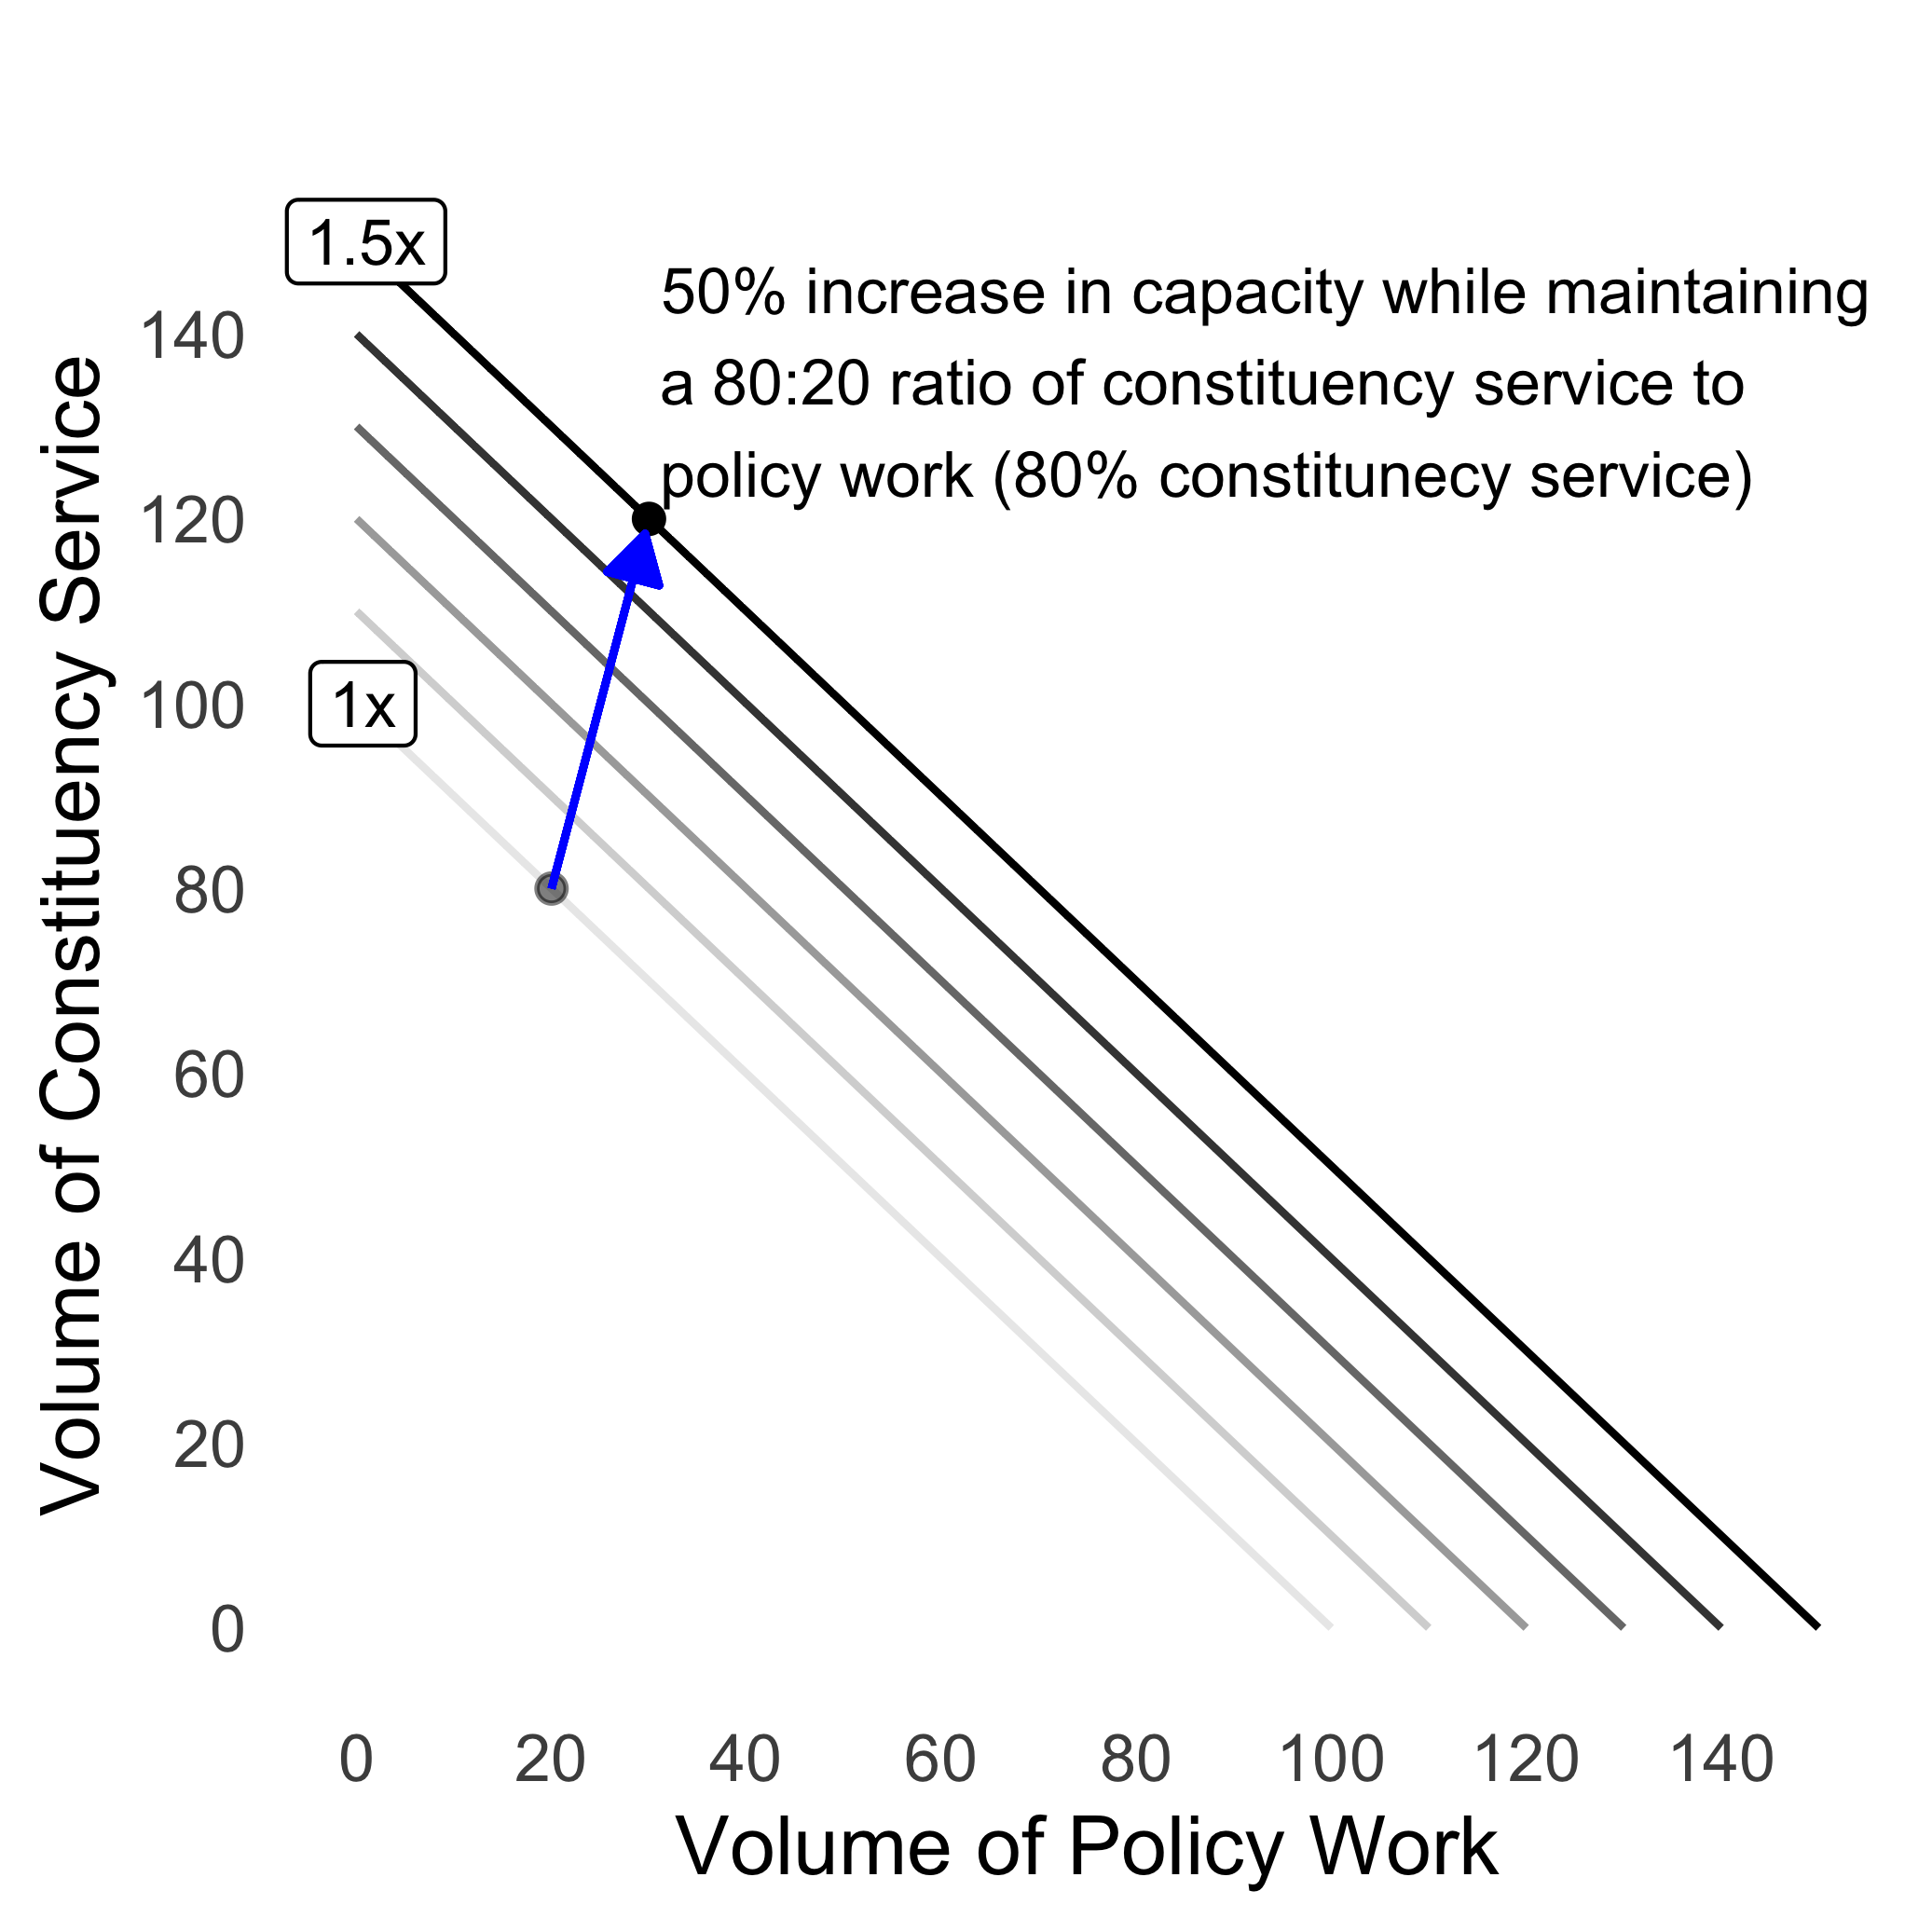
\includegraphics[width = \textwidth]{figs/2x2-fig-1}
\footnotetext{This figure is a visual representation of the potential outcomes implied by the formalization of our theory. The figure assumes a baseline capacity of 100 (e.g., 100 contacts with federal agencies per year) and a baseline ratio of constituency service to policy work of 80:20 (80\% constituency service). Subfigure 1 (Upper Left Quadrant) shows what happens if capacity increases by 50\%, and no shift in priorities. Subfigure 2 (Upper Right Quadrant) shows what happens if priorities shift from 80:20 to 60:40 constituency service to policy work, and there's no shift in capacity. Subfigure 3 (lower left quadrant) shows what happens if both capacity increases by 50\% and priorities shift from 80:20 to 60:40. If both capacity increases and priorities shift, the net outcome on volume of constituency service and volume of policy work depends on exactly how much each changes. Subfigure 4 (lower right quadrant) illustrates the range of possibilities that could occur when both capacity increases and priorities shift. Subfigure 3, is just one possible scenario of this more general form. }
\end{minipage}
\end{figure}

Figure \ref{f:2x2-fig} formalizes the potential outcomes implied by our theory to clarify the conditions under which constituency service will increase or decrease as an elected official's capacity and priorities change. 
For simplicity, Figure \ref{f:2x2-fig} assumes a baseline capacity of 100 (e.g., 100 contacts with federal agencies per year) and a baseline ratio of constituency service to policy work of 80:20 (80\% constituency service). It visualizes potential outcomes for changes in capacity extending up to 150\% of some baseline level of capacity.
The level of policy work, $x$, done by an elected official, $i$, depends on their overall capacity, $c$, and relative priority for constituency service versus policy work, $p \in [0, 1]$ (that is, the share of contacts that are constituency service rather than policy work) such that $x_i = c_i (1-p_i)$.
An elected official's level of constituency service, $y_i$, likewise depends on their overall capacity and priorities such that $y_i = c_i p_i$.
For any given level of capacity, $y_i = c_i-x_i$ specifies a line of possible divisions of capacity between policy work and constituency service. Increasing capacity pushes this "capacity frontier" line to the upper right (Figure \ref{f:2x2-fig}, subfigure 1). Where on this line a legislator exists at any point in time depends on their relative priority for policy work and constituency service (Figure \ref{f:2x2-fig}, subfigure 2). If capacity and priorities shift simultaneously, priorities can shift toward policy while levels of constituency service are maintained or even increase (Figure \ref{f:2x2-fig}, subfigure 3). The relative magnitude of these two effects determines whether constituency service will increase or decrease (Figure \ref{f:2x2-fig}, subfigure 4).  
When $c_{i1}p_{i1} > c_{i2}p_{i2}$, constituency service decreases between time 1 and time 2. 
When $c_{i1}p_{i1} < c_{i2}p_{i2}$ constituency service increases. 
When $c_{i1}p_{i1} = c_{i2}p_{i2}$, there is no change in constituency service. 

\subsection{Alternative Explanation for Changes in Constituency Service: Constituent Demand}

We aim to understand how gaining power and experience in Washington affects how legislators serve constituents. But often, legislators depend on constituents to ask for help navigating the federal bureaucracy. An alternative explanation for why legislators' rates of constituency service provision vary is that they receive differing numbers of requests from their constituents for reasons that are not a result of legislators' capacity and experience. While such variation in constituent demand is substantively interesting, such an explanation for constituency service provision does not inform debates about the extent to which legislators' capacity and priorities change with their time in office and institutional position. 

Of course, constituent demands inform which agencies legislators contact. For example, some districts contain groups---such as veterans or social security recipients---who request particular kinds of constituency service from their representatives. \textbf{Our research design limits the influence of this kind of variation in constituent demand by examining how an individual legislator's rates of contact change \textit{within} each agency. By looking at the same member representing the same constituents in the same district to the same agency over time, we limit the extent to which differing constituent populations could interfere with our results.} 

Legislators may also use their official resources to encourage requests from constituents for help navigating the federal bureaucracy through workshops, newsletters to constituents, social media posts, and even stories in local papers. Such constituent outreach may even be a primary way that constituencies discover that their elected officials can help with problems they may have with the bureaucracy. If legislators use increased staff budgets or organizational capacities to solicit constituent requests, constituent demands may increase as legislator power increases \citep{CainFerejohnFiorina1987}.  %Increases in constituents' demands may thus reflect elected officials' capacity and efforts to solicit demand for constituency service.
This is entirely consistent with our theory that increased power and capacity enable legislators to provide both constituency services and policy work. Our theory and tests do not require that legislators allocate resources to soliciting constituency service demand as they gain power, but if they do, the underlying cause would be shifting legislator capacity, not some exogenous shift in constituent demand that could confound our analysis. Thus, changes in constituent demand that result from legislators' efforts are not a problem for our analysis. Indeed, constituent service outreach may be a key mechanism for the capacity effects we theorize.

A more challenging form of constituent demand could exist if constituents redirect their requests toward legislators whom they expect to be more powerful. Constituents might expect that more powerful legislators could more effectively provide constituency service and, as a result, direct their demands toward those legislators. If constituents strategically redirect their demands for help from representatives who lost a chair position to representatives who gained a chair position, this could partially confound our analysis. More realistically, if constituents redirect requests for help away from new legislators toward longer-serving legislators, we might observe increases in demand targeted at more experienced legislators of a delegation whenever a less experienced legislator replaces another more experienced member of their state's delegation.  
To address these sorts of concerns, in Section \ref{s:demand}, we conduct a series of robustness checks to rule out alternative constituency demand-driven explanations. We find no evidence of requests spilling over to more experienced and powerful members within a state delegation.  



%%%%%%%%%%%%%%%%%%%%%%%%%%%
%% DATA %%%%%%%%%%%%%%%%%%%
%%%%%%%%%%%%%%%%%%%%%%%%%%%

\section{Data: A Census of Legislator Requests to Federal Agencies} \label{s:data}
To assess how experience and power affect constituency service, we filed \input{tables/foia_requests} Freedom Of Information Act (FOIA) requests with all federal departments, agencies, and sub-agencies for all records of incoming communication from members of Congress between January 1, 2007, and the date of our request.\footnote{In addition to our initial requests, collecting these data included over a thousand follow-up and clarification emails, dozens of hours on the phone with FOIA officers, and nearly 100 appeals of incomplete records or inappropriate denials, including multiple cases where we pursued and won orders from judges requiring compliance with our request. By rigorously pursuing a census of records, we limit any response bias that may exist in more easily-obtained samples.} 
Between February 2017 and February 2021, we received data on \input{tables/n} instances of members of Congress contacting federal agencies. We focus on requests made from 2007 to 2020, resulting in a data set of  \input{tables/n2007-2020} contacts.\footnote{Some agencies did not provide records for the full span of years. Our models include legislator-by-agency fixed effects to account for any left censoring, ensuring that our comparisons leverage variation within each agency, limiting the opportunity for censoring to affect our results.} 



\paragraph{Data processing and coding} Upon receiving records of congressional requests, we extracted names matching variations of legislators' names. %TODO using the `legislators` R package \citep{legislators}. 
We then merged in data about members' districts, institutional positions, and careers, including ideology scores \citep{dwnominate2018}, committee membership \citep{StewartWoon2017}, and committee oversight \citep{LewisSelin2012}. %We also made a considerable effort to verify and update committee membership data. 
The Appendix provides procedures and replication code for converting the raw records from federal agencies into the data set required for our analysis. 

For \input{tables/n2007-2020coded} requests, we use the text or summaries of letters to classify legislators' reasons for contacting federal agencies. Our coding process began with the authors coding a representative sample of records using our codebook (see Appendix). We then trained Research Assistants to continue the coding. The first several thousand letters were double-coded. For example, of over 10,000 letters for the Environmental Protection Agency, the first 2,500 were double-coded. Our overall inter-coder agreement was 0.78, which rose to 0.9 when we subsetted our analysis to coding decisions where the coders had a great deal of certainty. 


\subsection{Who Contacts the Bureaucracy and Why?} \label{s:descriptive} 
Before testing theories of how legislators' efforts to provide constituency service change as they acquire experience and power, we first use our extensive new data set to answer outstanding descriptive questions about representation in U.S. politics. These descriptive findings regarding the level, variation, and reasons for legislator requests to federal agencies are only possible with our census of legislator requests. Overall, we find massive variation across legislators. We also find surprising consistency in the purpose of the communication; when legislators contact federal agencies, it is almost always to provide constituency service; only a small fraction focused on policy work. Further, we find that legislators are responsive to their constituency's demographic characteristics, but there is still significant variation in levels of service from similar districts.  

\subsubsection{Legislator's Contact with Federal Agencies Focus on Constituency Service}
Overall, when legislators contact federal agencies, they are helping constituents navigate the federal bureaucracy. Figure \ref{f:type2} shows the proportion of contacts for each of the five types of legislator requests in our hand-coded sample described above. The center bar shows that 71\% of all legislator requests to federal agencies are on behalf of individual constituents. Constituent service requests on behalf of individual corporations are a smaller percentage, 6\%. 7\% of requests are on behalf of nonprofits and local governments. General policy work and policy work on behalf of specific industries account for just 16\% of all requests made to federal agencies.  


\begin{figure}[hbt!]
\centering
\caption{Legislator Requests to Federal Agencies by Type 2007-2018} \label{f:type2}
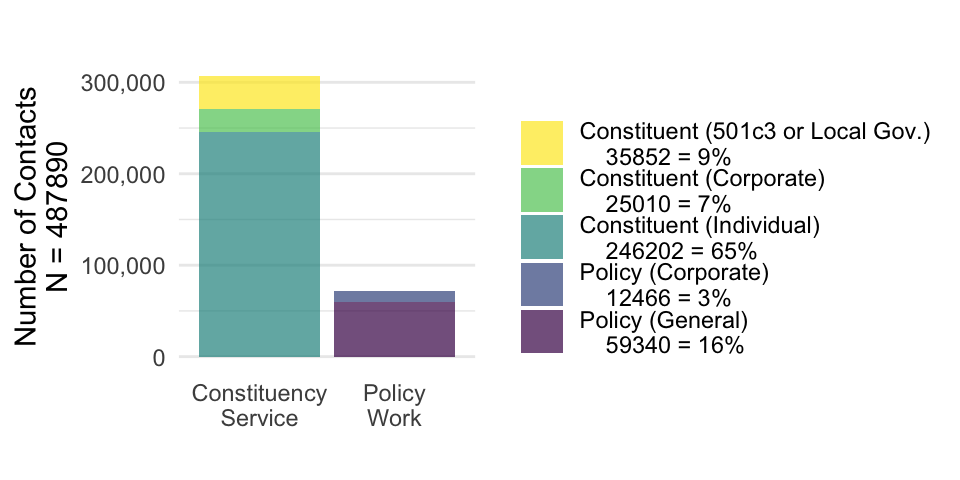
\includegraphics[width = .8\textwidth]{figs/data_by_type-tall-1}
\end{figure}



To assess whether legislators shift their priorities as they gain experience and power, we further group requests into a broader ``constituency service"  category (including service for individuals, corporations, and nonprofits) and ``policy work" category (including both general and industry-focused policy work) for our tests in section \ref{s:prestige}. We find that 76\% of requests from committee chairs are constituency service (compared to 85\% for non-chairs). %84\% of requests from members of prestige committees are constituent service (compared to 83\% for members of non-prestige committees). 
Descriptively, most legislator requests are constituency service. However, legislators in more powerful positions have a higher ratio of policy work to constituency service.\footnote{We say that a House member is on a prestige committee if they are on Appropriations, Ways and Means, Rules, Budget, or Armed Services and if a senator is on Rules, Foreign Relations, Commerce, Budget, Armed Services, or Appropriations.} %CITE? 


\subsubsection{Levels of Contact with Federal Agencies are Highly Unequal}
Legislators vary significantly in how often they contact federal agencies. Gini coefficients for the number of contacts per year for the House and Senate are similar to those for income inequality in Mexico and the United States, respectively. Figure \ref{f:contact1} shows the average number of contact rates per year for House members (left-hand panel) and senators (right-hand panel). Senator James Webb (D-VA) averaged 533 contacts per year. %Other senators---including Kirsten Gillibrand, (D-NY), Charles Schumer (D-NY), and Marco Rubio (R-FL)---have similarly high levels of contact with federal agencies. But other senators contact at a much lower rate. 
On average, senators in our data contacted agencies 117 times per year.   
 
\begin{figure}
\centering
\caption{Variation in Average Legislator Requests by Percentile} \label{f:contact1} 
\begin{minipage}{\textwidth}
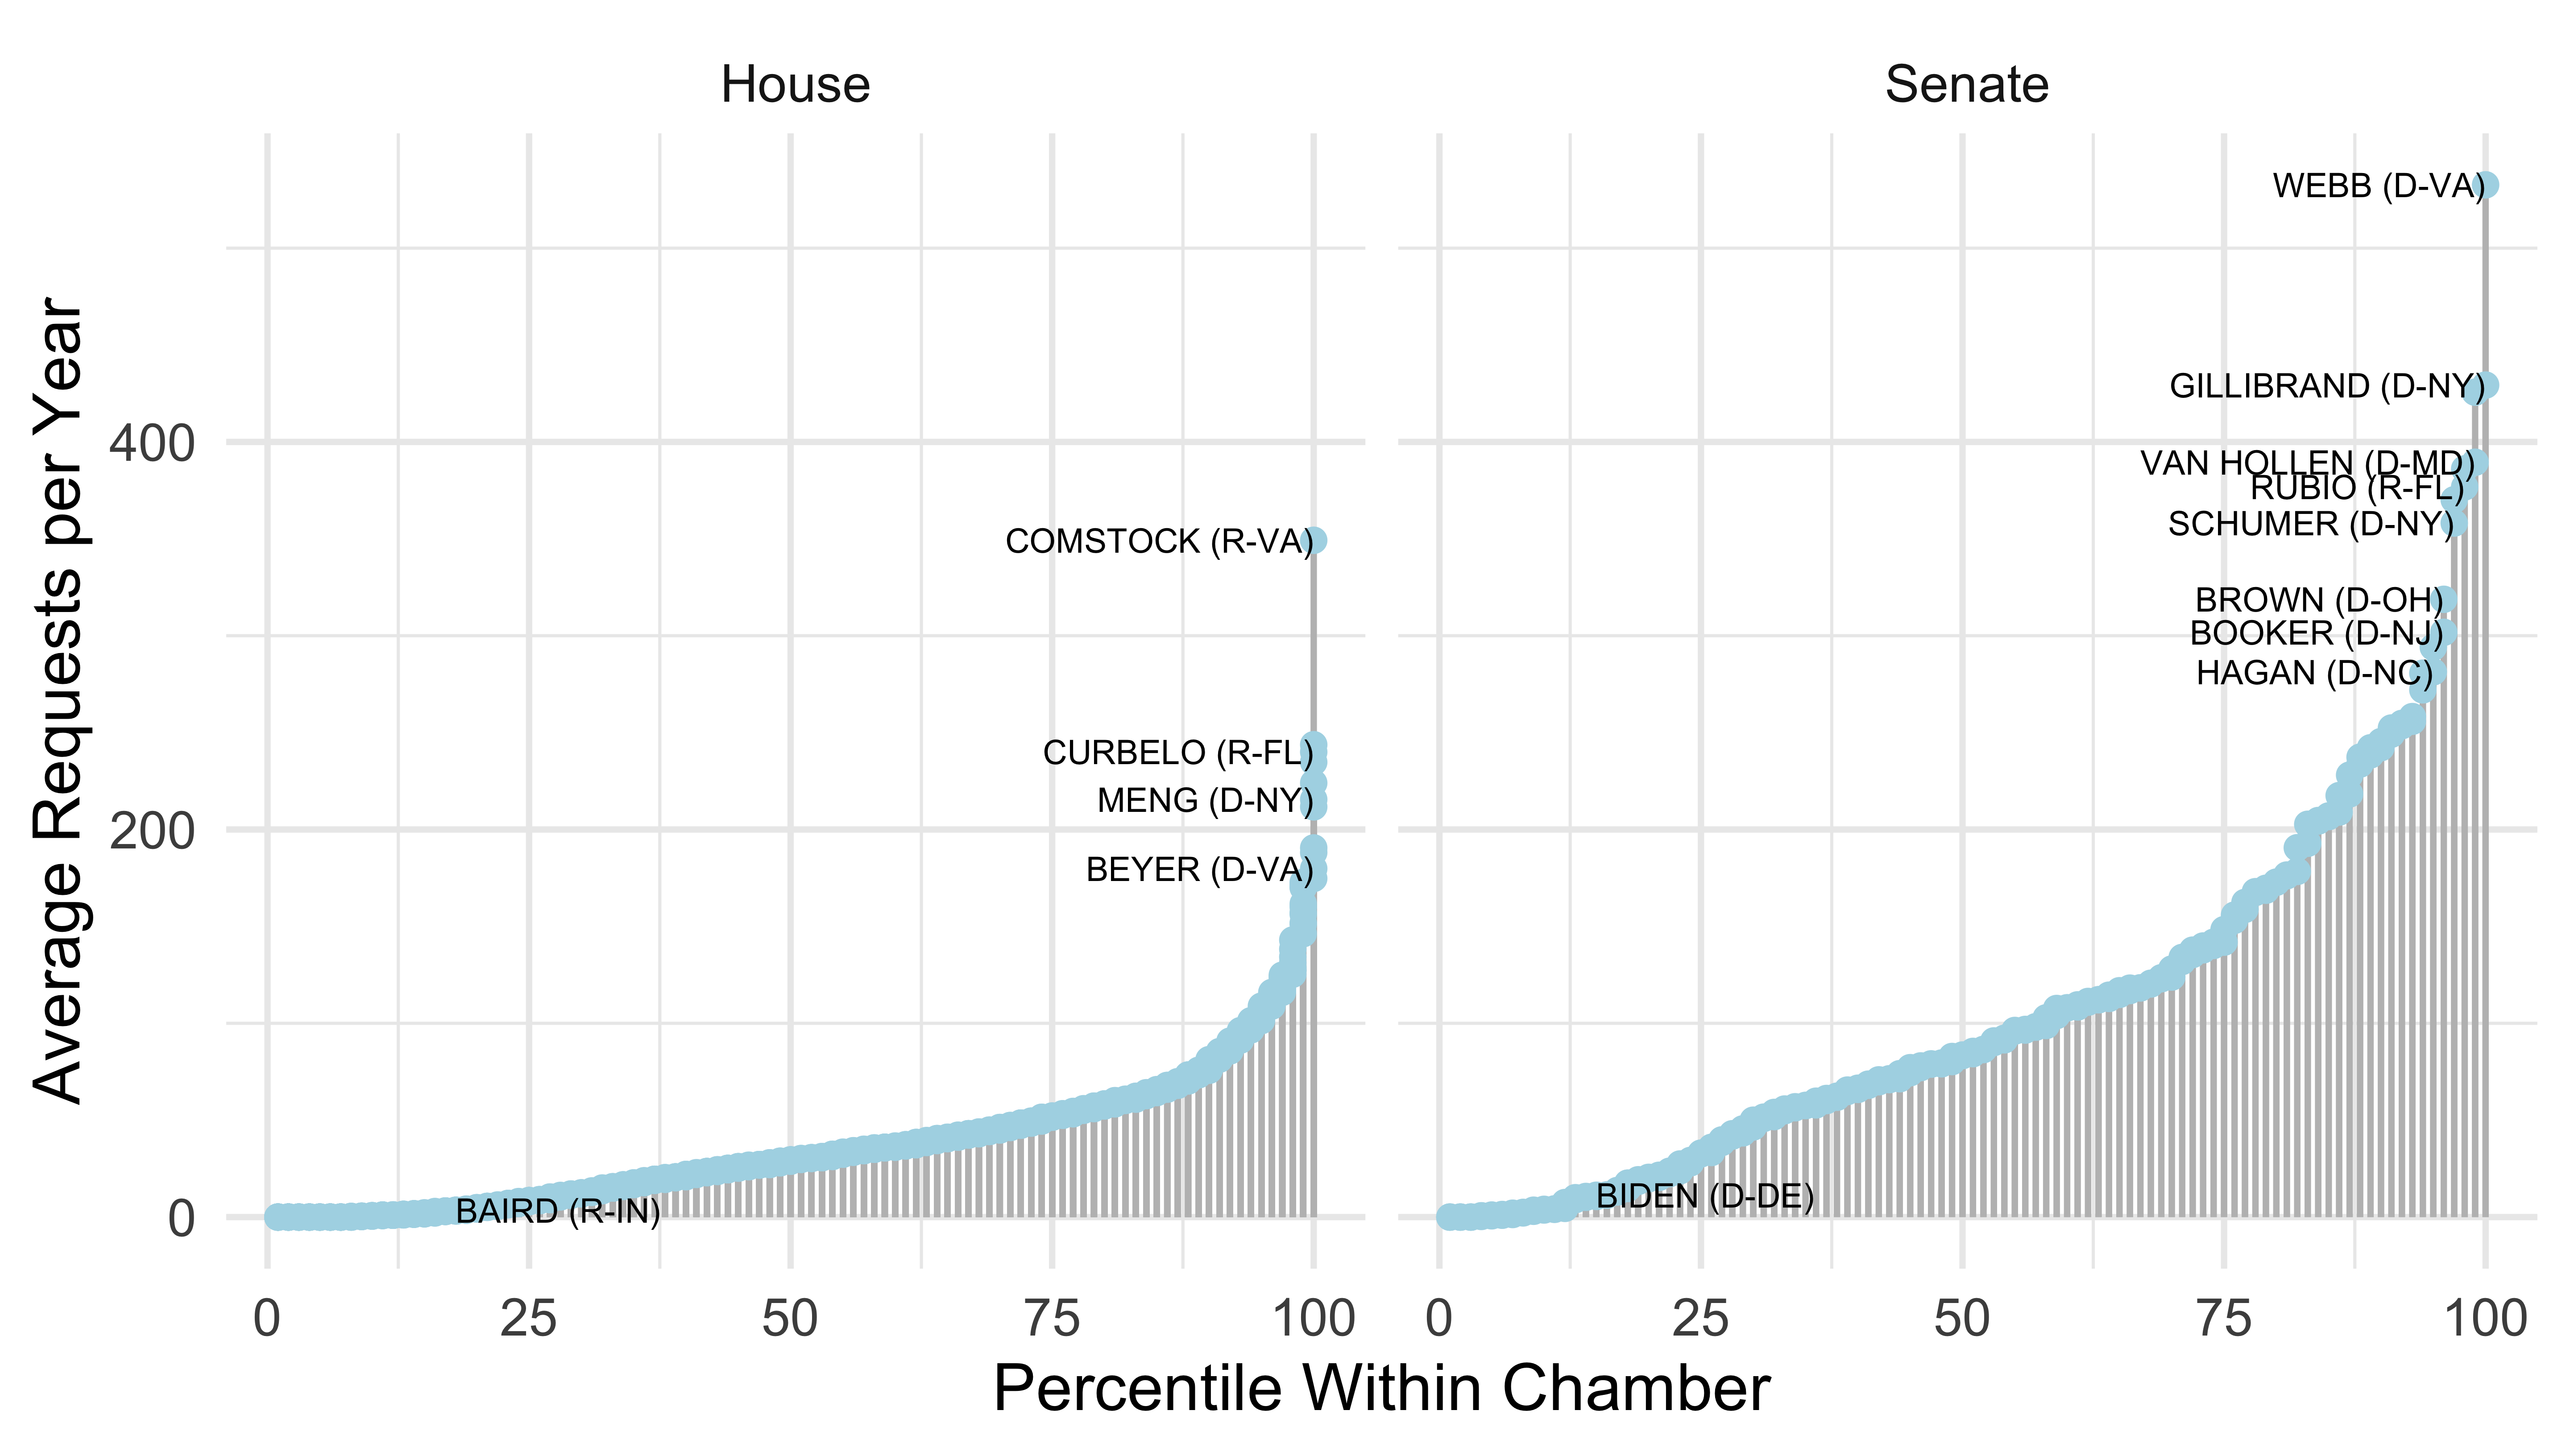
\includegraphics[width = \textwidth]{figs/percentiles-1}
\footnotetext{This figure presents the average number of contacts with federal agencies per year for House members (left-hand panel) and senators (right-hand panel), where the legislators' counts are sorted by their per year percentile rank. This reveals that senators and House members regularly contact federal agencies, but there is considerable variation in the level of contact across legislators.}
\end{minipage}
\end{figure}


We see a similar level of variation in the House, but with lower overall levels of contact with federal agencies, reflecting lower resources and fewer constituents than senators. Frank Wolf (R-VA) averaged 377 contacts per year. Like the Senate, other members of the House wrote at much lower rates. For example, in her first year in Congress,  Michele Bachmann wrote only six letters in our data but would average 31 letters per year by the end of her time in Congress. Overall, House members averaged 52 contacts with federal agencies per year. But like the Senate, we find massive variation in the levels of contact across House members.  

Figure \ref{f:peryear} shows the number of requests per legislator over time, highlighting three Senators at the upper, middle, and lower parts of the distribution.

\begin{figure}
\centering
\caption{Variation in Legislator Requests by Year 2007-2017} \label{f:peryear} 
\begin{minipage}{\textwidth}
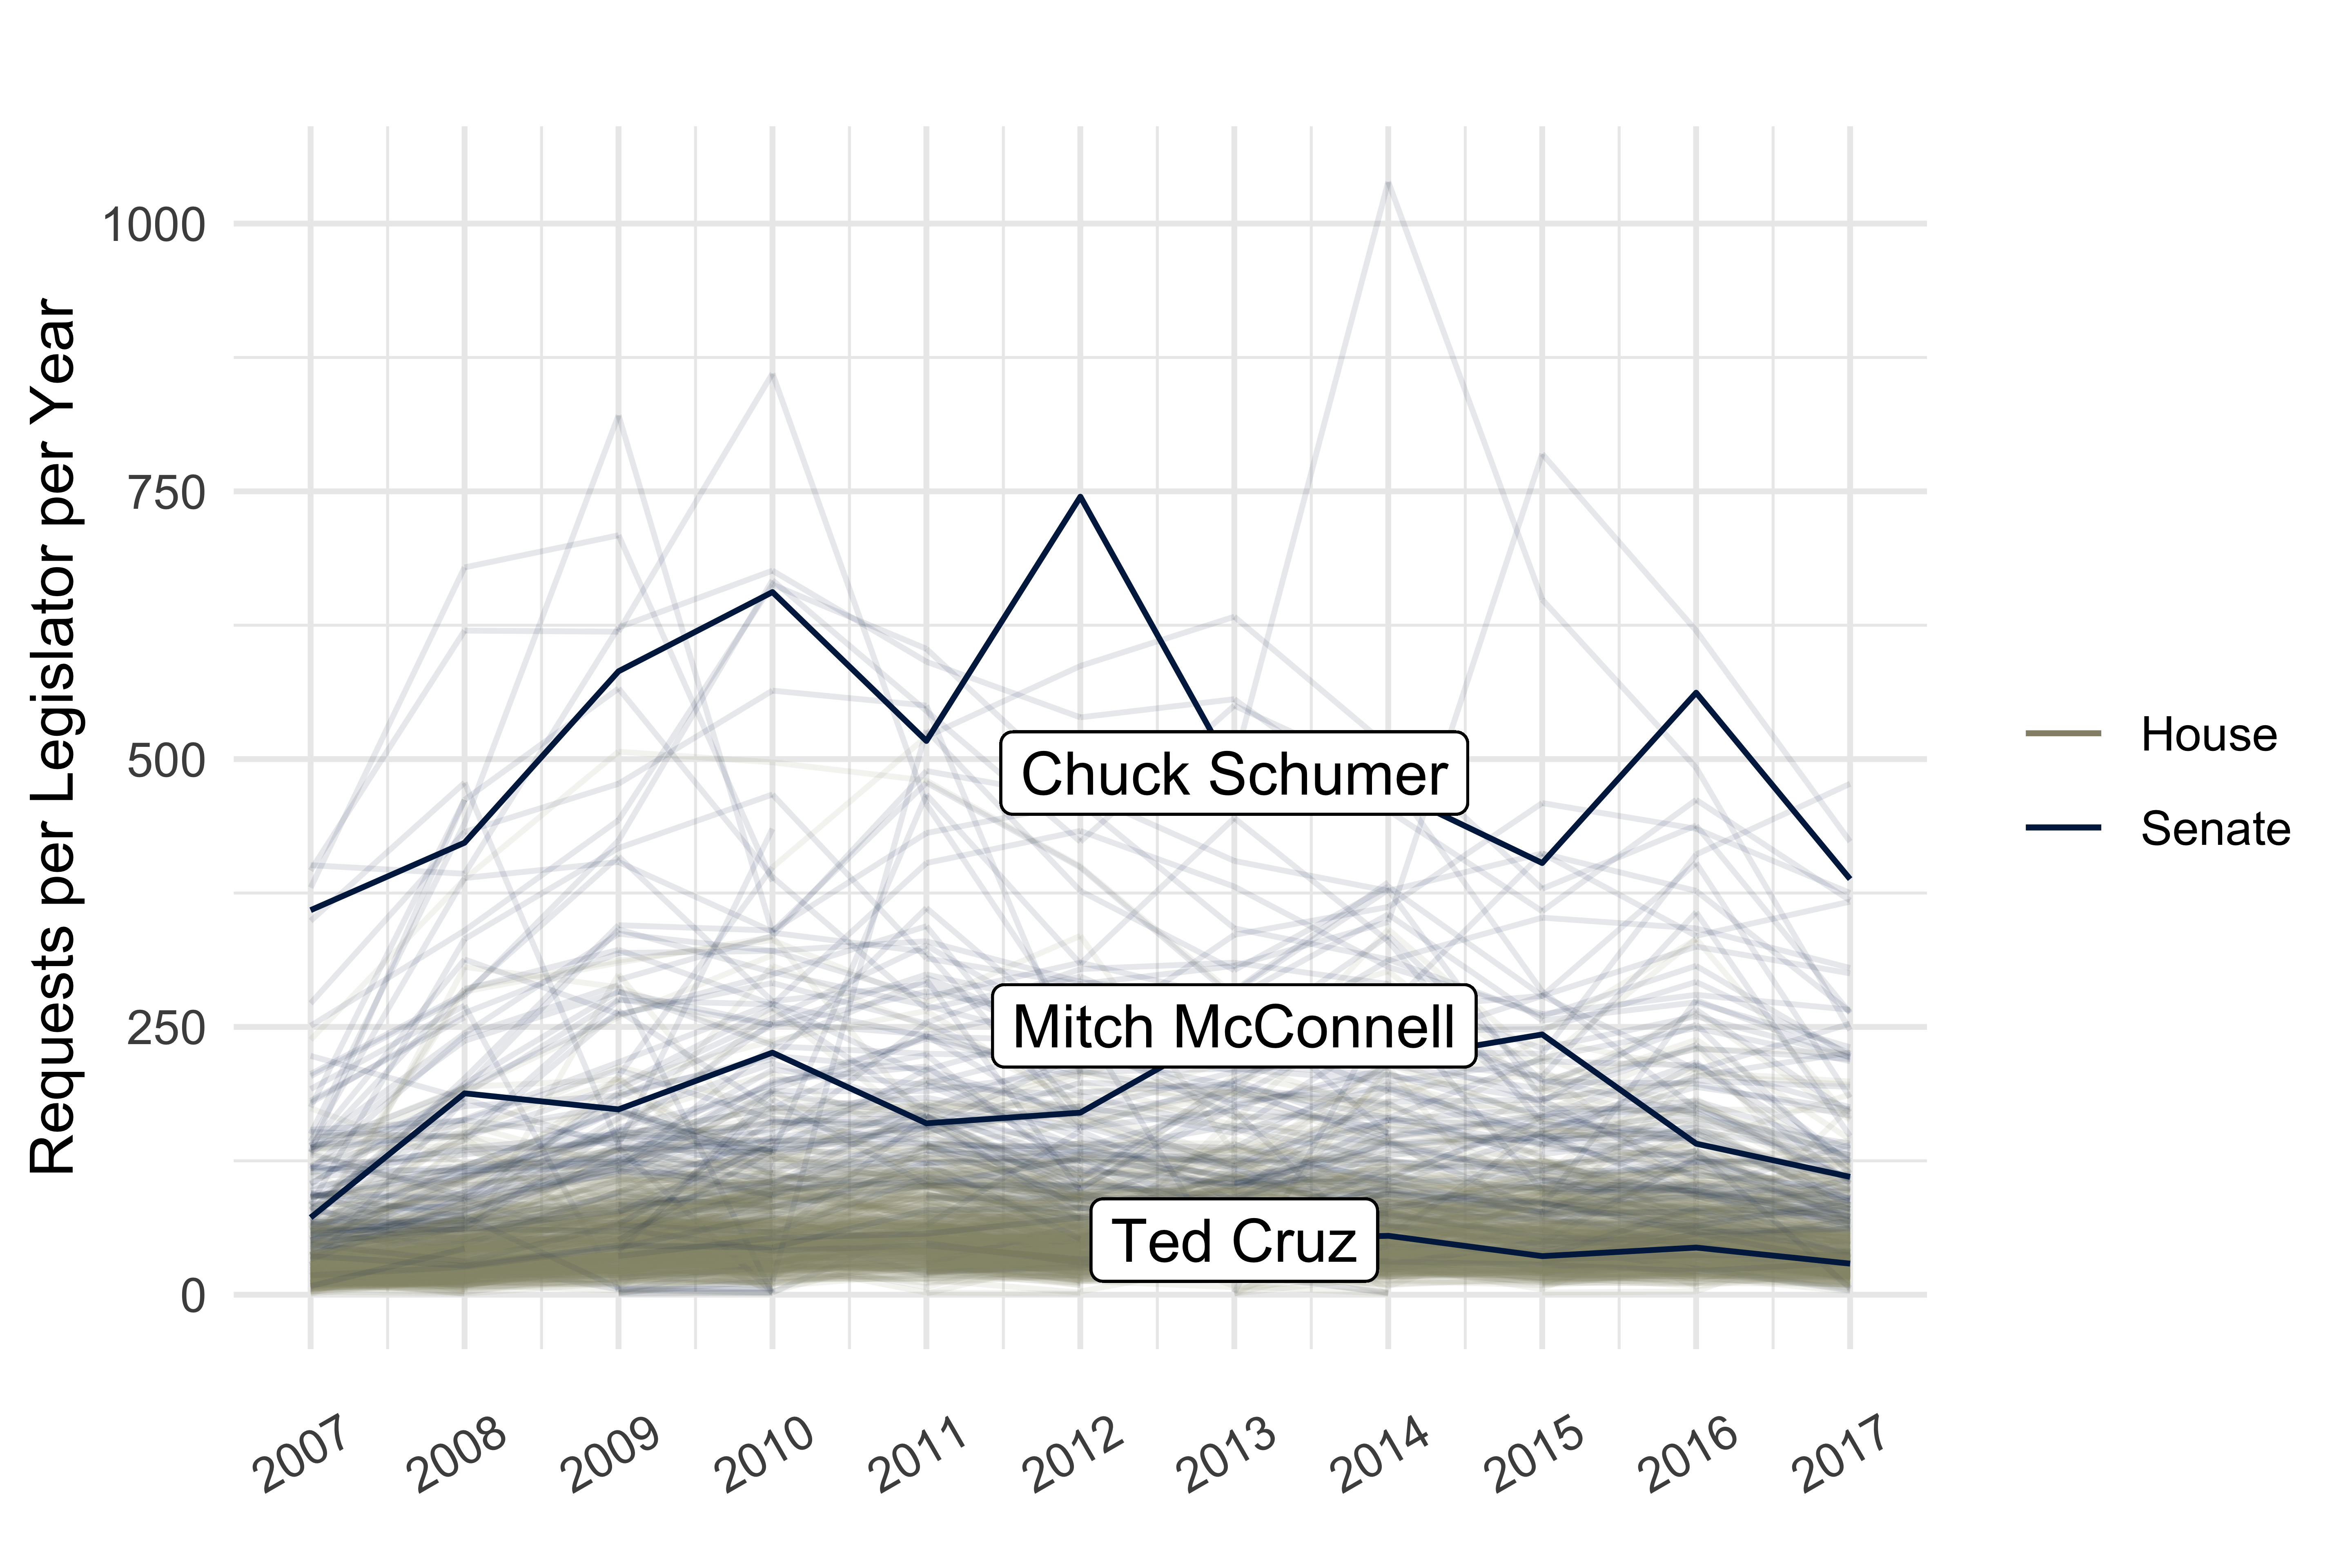
\includegraphics[width = \textwidth]{figs/counts-per-year-1}
\footnotetext{This figure presents the number of contacts with federal agencies per year for House members (left-hand panel) and senators (right-hand panel) over time. This reveals that senators and House considerable variation in the level of contact both within and across legislators.}
\end{minipage}
\end{figure}




\section{The Effect of Experience and Institutional Power}\label{s:results} 

Using this dataset of requests to federal agencies, we estimate the effect of institutional power on legislator behavior. First, we test theories rooted in legislator capacity by modeling the effects of institutional power on a legislator's overall \textit{level} of constituency service. Next, we test theories rooted in legislators' priorities by modeling the effects of institutional power on a legislator's  \textit{ratio} of policy work to constituency service. %Finally, we estimate the combined substantive impact of increasing capacity and shifting priorities. 

\subsection{The Effects of Experience and Institutional Power on Levels of Constituency Service}\label{s:prestige}

Our primary models are difference-in-differences regressions, similar to the specifications in \cite{BerryFowler2016}. Our most stringent specifications examine changes within legislator-agency pairs (Equation \ref{e:diff1}).\footnote{We drop five member-congress level observations for congresses where members switched political parties.} 

\begin{eqnarray}
Y_{ijt} & = & \boldsymbol{\beta}^{'} \textbf{Committee Position}_{it}  + \sum_{s = 1}^{6} \eta_{s} \text{I}\left(\text{tenure}_{it} = s\right) + \gamma_{ij} + \delta_{jt} + m_{it} + p_{it} + \epsilon_{ijt} \label{e:diff1}
\end{eqnarray}

Our analysis in this section is at the legislator-agency-year level. $Y_{ijt}$ is the number of requests legislator $i$ makes to agency $j$ in year $t$. $\gamma_{ij}$ is a fixed effect for the legislator-agency pair. This fixed effect controls for legislators' characteristics, such as legislators who are more skillful at filling constituency service requests than others. Critically for our research design, this fixed effect also \textbf{accounts for time-invariant constituent demand}, ensuring that differences in constituent requests across legislators do not drive our results. It also accounts for state and district characteristics, including population, demographics, and local industries that might be particularly likely to request help from specific agencies. This difference-in-difference design ensures that coefficients $\boldsymbol{\beta}$ capture variation related to changes in institutional power, not other factors that may vary across districts, legislators, or agencies. The model also accounts for the different periods for which data were available from each agency. $\delta_{jt}$ is an agency-year fixed effect. This takes into account agency-specific shocks that may affect legislator requests. 

Assuming that legislators' trends in the number of requests to a given agency follow parallel paths over time, $\boldsymbol{\beta}$ represents the average effect of changing institutional position on a legislator's provision of constituency service. We focus on three measures of a legislator's position: (1) whether they are a committee chair, (2) whether they are a ranking member of a committee, and (3) whether they are members of a prestige committee. Each position represents a different way legislators can acquire more power. As a legislator becomes a committee chair or ranking member, they have increased responsibilities when drafting and revising legislation. They also have increased access to committee resources to accomplish policy goals, particularly the power to direct committee staff. Similarly, legislators who join more prestigious committees gain opportunities to shepherd policy through the legislative process.

As \cite{BerryFowler2016} note, changes in legislators' committee assignments are often due to circumstances outside of the legislator's control, such as changing majority status, retirements on a committee, or exclusion due to losses from a previous election \citep{GrimmerPowell2013}. To violate the parallel trends assumption,  legislators must differentially alter their provision of constituency service in anticipation of joining particular committees. To help avoid this violation, we include a series of controls that capture time-varying characteristics of a legislator that might confound our inference about the effect of committee prestige. Because legislators may make more requests to a president of the same party \citep{BerryBurdenHowell09}, it is a particular concern that legislators obtain new committee assignments when their party moves into or out of the majority or at the same time as the president's party changes. To address these concerns, we include indicators for whether the legislator's party is the majority in year $t$, ($m_{it}$) and if the legislator is from the same party as the president in year $t$ ($p_{it}$). Throughout, we cluster standard errors at the legislator level.

We also include indicators for legislators' first six years in Congress, $ \sum_{s = 1}^{6} \eta_{s} \text{tenure}_{it}$ as controls.
%The effects of interest $\eta_{1}, \eta_{2}, \hdots, \eta_{6}$ describe how a legislator's provision of constituency service at levels of seniority between one and six years differ from legislators who serve beyond six years. We focus on constituency service levels in the first six years of a legislator's tenure to assess how constituency service changes over their initial years in Congress. This design allows us to assess whether new legislators face start-up costs. 
This specification, however, is not the best specification to assess how electing a less experienced representative affects the amount of constituency service a district receives. In Section \ref{s:tenure_dist}, we test the effect of legislator experience by estimating how electing a new representative affects the number of constituency service requests made on behalf of a district with a different difference-in-differences specification at the district level.   

%\subsection{The Effects of Experience and Institutional Power on the Level of Constituency Service} 


\subsubsection{The Effect of Institutional Power on Levels of Constituency Service}\label{s:prestigeresults}

\begin{table}[hbt!]
\caption{The Effect of Experience and Institutional Power on Constituency Service} \label{t:models_total}
\begin{minipage}{\textwidth}
\begin{center}
% \begin{tabular}{l*{4}{c}}
\toprule
                    &\multicolumn{1}{c}{(1)}&\multicolumn{1}{c}{(2)}&\multicolumn{1}{c}{(3)}&\multicolumn{1}{c}{(4)}\\
\midrule
Committee Chair     &       0.712&       0.206&       0.209&      0.0366\\
                    &     (0.152)&    (0.0951)&    (0.0951)&    (0.0136)\\
Ranking Member      &       0.852&       0.123&       0.136&      0.0250\\
                    &     (0.156)&    (0.0967)&    (0.0970)&    (0.0119)\\
Prestige Committee  &       0.470&      0.0790&      0.0746&      0.0210\\
                    &    (0.0665)&    (0.0508)&    (0.0519)&    (0.0103)\\
First Year          &      -0.255&      -0.139&      -0.144&     -0.0124\\
                    &    (0.0519)&    (0.0489)&    (0.0473)&   (0.00979)\\
Second Year         &     -0.0713&      0.0177&      0.0248&      0.0239\\
                    &    (0.0585)&    (0.0474)&    (0.0469)&   (0.00908)\\
Third Year          &     -0.0198&      0.0764&      0.0595&      0.0338\\
                    &    (0.0625)&    (0.0450)&    (0.0444)&   (0.00823)\\
Fourth Year         &     0.00126&      0.0707&      0.0522&      0.0260\\
                    &    (0.0664)&    (0.0455)&    (0.0431)&   (0.00806)\\
Fifth Year          &     -0.0515&      0.0280&      0.0266&      0.0164\\
                    &    (0.0611)&    (0.0377)&    (0.0367)&   (0.00701)\\
Sixth Year          &     -0.0156&      0.0504&      0.0744&    0.000378\\
                    &    (0.0728)&    (0.0536)&    (0.0516)&   (0.00762)\\
\midrule
Majority, President's Party&  \checkmark&  \checkmark&  \checkmark&  \checkmark\\
Legislator $\times$ Agency Fixed Effects&            &  \checkmark&  \checkmark&  \checkmark\\
Year $\times$ Agency Fixed Effects&            &  \checkmark&  \checkmark&  \checkmark\\
All Legislators     &  \checkmark&  \checkmark&            &  \checkmark\\
Serve At Least Second Term&            &            &  \checkmark&            \\
Dependent Variable  &       Count&       Count&       Count&Log(Count + 1)\\
Observations        &      412111&      412111&      388997&      412111\\
\bottomrule
\multicolumn{5}{l}{\footnotesize Robust standard errors in parentheses, clustered at legislator level}\\
\end{tabular}
 % stata table was missing FE
\begin{table}
\centering
\begin{tabular}[t]{lcccc}
\toprule
  & 1 & 2 & 3 & 4\\
\midrule
Dependent Variable & Count & Count & Count & Log(Count+1)\\
Committee Chair & \num{0.712} & \num{0.271} & \num{0.275} & \num{0.049}\\
 & (\num{0.152}) & (\num{0.090}) & (\num{0.090}) & (\num{0.012})\\
Ranking Member & \num{0.852} & \num{0.153} & \num{0.170} & \num{0.031}\\
 & (\num{0.156}) & (\num{0.094}) & (\num{0.094}) & (\num{0.010})\\
Prestige Committee & \num{0.470} & \num{0.100} & \num{0.093} & \num{0.026}\\
 & (\num{0.067}) & (\num{0.051}) & (\num{0.052}) & (\num{0.010})\\
First Year & \num{-0.255} & \num{-0.512} & \num{-0.494} & \num{-0.103}\\
 & (\num{0.052}) & (\num{0.075}) & (\num{0.073}) & (\num{0.012})\\
Second Year & \num{-0.071} & \num{-0.275} & \num{-0.291} & \num{-0.042}\\
 & (\num{0.058}) & (\num{0.072}) & (\num{0.072}) & (\num{0.011})\\
Third Year & \num{-0.020} & \num{-0.189} & \num{-0.208} & \num{-0.030}\\
 & (\num{0.063}) & (\num{0.061}) & (\num{0.060}) & (\num{0.009})\\
Fourth Year & \num{0.001} & \num{-0.135} & \num{-0.158} & \num{-0.018}\\
 & (\num{0.066}) & (\num{0.060}) & (\num{0.057}) & (\num{0.009})\\
Fifth Year & \num{-0.052} & \num{-0.135} & \num{-0.139} & \num{-0.024}\\
 & (\num{0.061}) & (\num{0.043}) & (\num{0.042}) & (\num{0.007})\\
Sixth Year & \num{-0.016} & \num{-0.029} & \num{-0.011} & \num{-0.014}\\
 & (\num{0.073}) & (\num{0.056}) & (\num{0.054}) & (\num{0.007})\\
Majority & \num{0.134} & \num{0.020} & \num{0.025} & \num{-0.012}\\
 & (\num{0.052}) & (\num{0.033}) & (\num{0.033}) & (\num{0.004})\\
President's Party & \num{0.112} & \num{0.037} & \num{0.042} & \num{0.012}\\
 & (\num{0.057}) & (\num{0.027}) & (\num{0.027}) & (\num{0.004})\\
\midrule
All Legislators & ✓ & ✓ &  & ✓\\
Served At Least Second Term &  &  & ✓ & \\
Num.Obs. & \num{412111} & \num{412111} & \num{388997} & \num{412111}\\
Std.Errors & by: Legislator & by: Legislator & by: Legislator & by: Legislator\\
Legislator x Agency Fixed Effects &  & ✓ & ✓ & ✓\\
Year x Agency Fixed Effects &  & ✓ & ✓ & ✓\\
\bottomrule
\end{tabular}
\end{table}
 % this one is from replication.rmd
\end{center}
\footnotetext{This table shows how the number of contacts changes as legislators acquire more experience and power. Column 1 shows the average differences across committee assignments and years in Congress. Column 2 presents the difference-in-differences estimates. Column 3 subsets to legislators who serve at least three years. Column 4 takes the Log of the counts + 1 as the dependent variable.}
\end{minipage}
\end{table}

Table \ref{t:models_total} shows estimates from Equation \ref{e:diff1}. All coefficients represent the average additional requests per year \textit{per agency}; per legislator per year effects are simply these coefficients times \input{tables/n_agencies} (the number of agencies).
% IN THE RAW DATA, THERE ARE \input{tables/n_agencies} AGENCIES, BUT MAYBE SOME GET DROPPED? 



Model 1 (the first column of Table \ref{t:models_total}) shows a cross-sectional comparison across legislators. Legislators with more institutional power have higher rates of constituency service. %Model 1 excludes the legislator-agency and year-agency fixed effects but controls for majority status and being from the same party as the president.
Committee chairs, ranking members, and members of prestige committees %and oversight committee members 
provide substantially more constituency service than other legislators. However, these cross-sectional differences may be the result of other legislator characteristics. If legislators who are better at their jobs or exert more effort also receive more prestigious committee positions, then the estimates from Model 1 confound legislators' overall ability with their institutional position.   

To address potential confounding, Model 2 (Column 2 of Table \ref{t:models_total}) shows the difference-in-differences specification in Equation \ref{e:diff1}. Across all measures of institutional power, we find that acquiring power increases the number of requests that a given legislator makes. Becoming a committee chair causes an increase of  0.29 requests \textit{per agency} (95-percent confidence interval [0.12, 0.47]). Across all \input{tables/n_agencies}, this represents an increase of approximately 27 additional requests per year, 21.3\% of the average requests per year in our data. %There is a smaller increase for individuals who become ranking members and those who join a Prestige Committee, though the increase is statistically significant for the prestige committee. Becoming a ranking member of a committee causes an increase of 0.16 contacts per agency, while joining a prestige committee causes a 0.29 per agency increase in the number of contacts a member of Congress makes.

%We estimate that the experience gained between the first and second year in Congress causes an increase of 0.11 requests \textit{per agency}. The experience gained between the first and seventh year causes an increase of 0.43 per agency. Across all n_agency agencies, this represents an increase of approximately 39 additional requests per year, 31.2\% of the average requests per year in our data. There is a smaller increase after the second year. The experience gained between the second and seventh year causes an increase of 0.32 per agency, an increase of approximately 29 additional requests per year, 23.2\% of the average requests per year in our data.



\begin{figure}[hbt!]
\centering
\caption{Predicted Number of Total Letters (Within Legislator Difference in Differences) 2007-2018} \label{f:m-total-predicted}
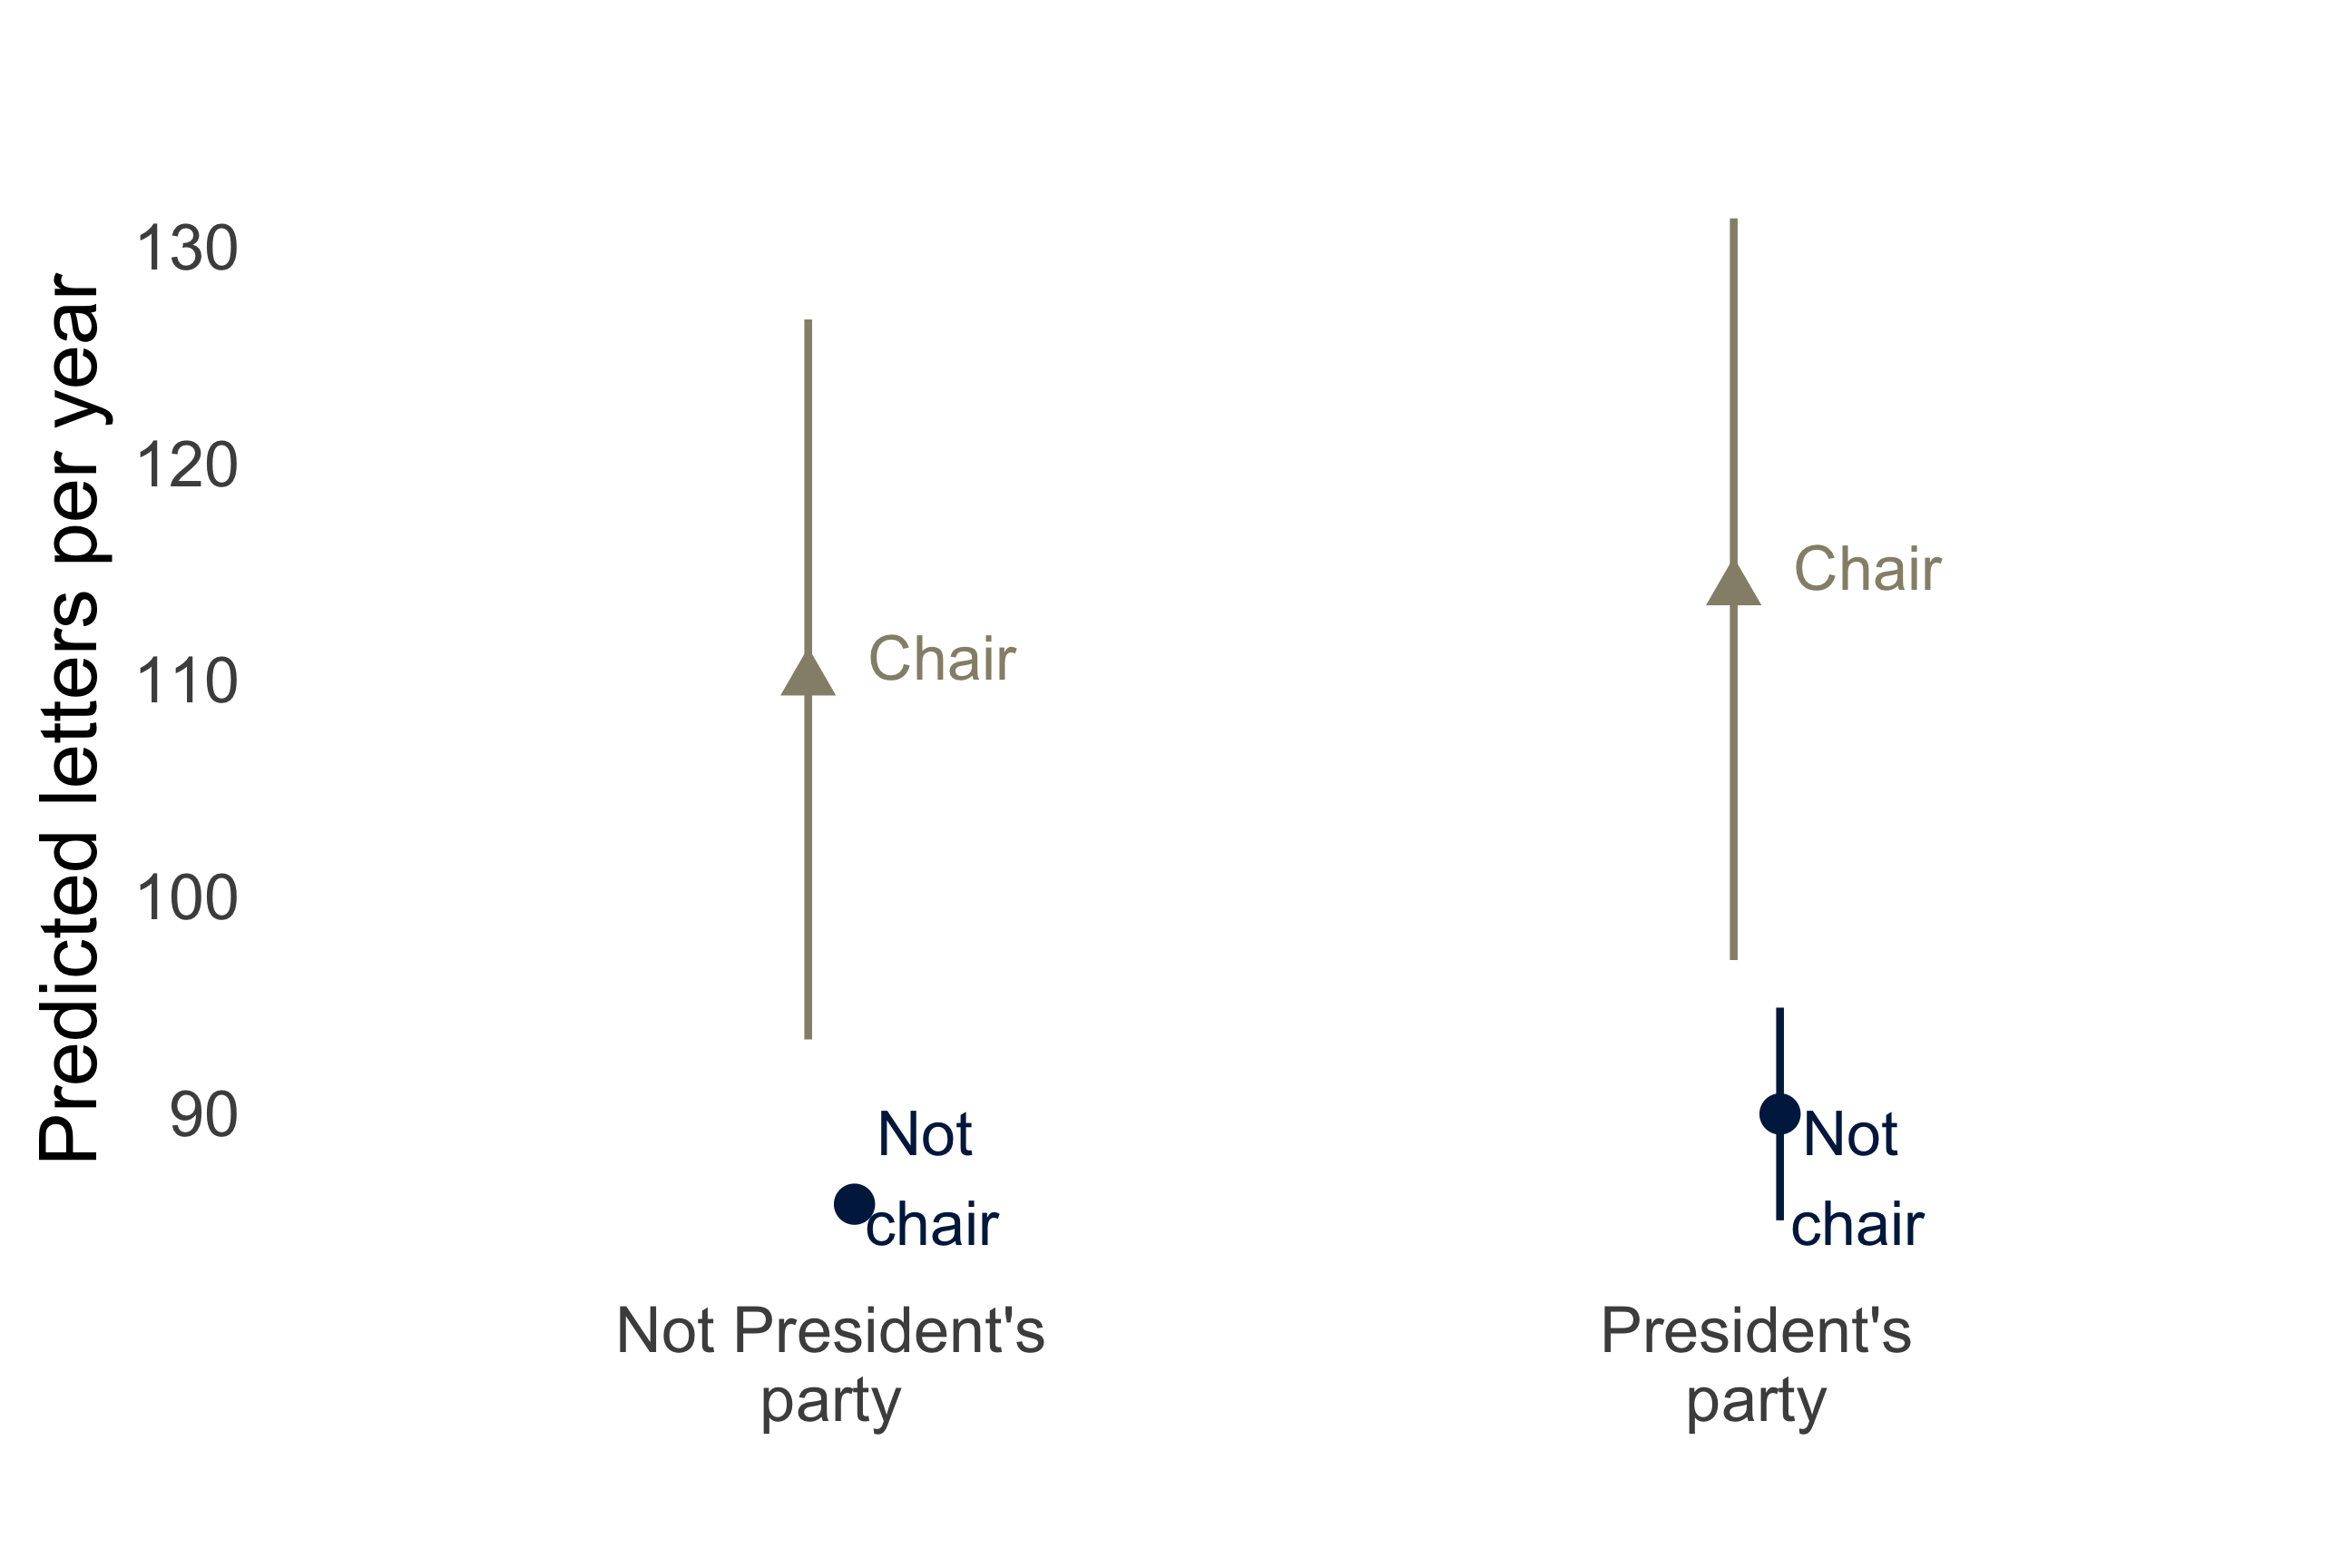
\includegraphics[width = .8\textwidth]{figs/m-total-predicted-3}
\end{figure}

Figure \ref{f:m-total-predicted} shows the predicted total number of letters per year by whether a legislator is a member of the president's party and whether they are a chair (comparing predictions for counterfactuals where the same legislator did and did not receive a chair position in their sixth year).\footnote{Predictions are based on a legislator-agency pair where (1) the legislators' average annual contacts equaled the overall average, (2) the legislators' number of contacts with the agency equal the average received by that agency, (3) and the agency received an average number of letters.} 
% legislators make significantly fewer requests to agencies in their first year than the following year. Subsequent increases are less significant. However, t
There is a significant increase when a legislator becomes a committee chair. There is no significant difference when a member has a co-partisan president.

The findings in Table \ref{t:models_total} are robust to alternative specifications and measures of the dependent variable. For example, we might be concerned that exceptionally productive legislators drive the results. The fourth column shows we obtain the same findings if we use $\log (Y_{ijt} + 1)$ in our difference-in-differences specification. Further, our results are not due to differential attrition. The third column shows that we obtain nearly identical results if we restrict our analysis to legislators who serve beyond three years.    

This section has shown that acquiring institutional power causes legislators to increase constituency service levels. This increase occurs across all three measures of committee position that we examine but is most robust for committee chairs. 


\subsubsection{The Effect of Legislator Experience on Levels of Constituency Service}\label{s:tenure} 

%As legislators acquire more power, they do more constituency service. While this suggests that more powerful legislators are paying more attention to their constituents, it could still be the case that legislators decrease their constituency service provision the longer they spend in office. To test whether this is the case, we use the estimates in Table \ref{t:models_total} but now focus on the coefficients in legislators' first six years in office. The reference group is representatives who have served longer than six years.\footnote{Interpreting these coefficients requires that we assume the effects of tenure and committee assignment are linearly separable. This assumption is reasonable because most legislators do not become chairs, ranking members, or join prestige committees in their first six years, and almost none in their first two years.} 

%The first column of Table \ref{t:models_total} shows large cross-sectional differences: legislators in their first year make fewer contacts than more experienced legislators. First-year legislators make approximately 0.255 fewer requests per agency than legislators in their seventh year or beyond. This difference shrinks in the second year and then is mostly gone. But we advise caution in interpreting the differences in Column 1 because they conflate the effect of increased experience with other characteristics that may correlate with whether a legislator remains in office and, thus whether we observe them in later years.   

%To account for possible differences in legislators who obtain different levels of tenure, the second column of Table \ref{t:models_total} estimates the difference-in-differences specification in Equation \ref{e:diff1}. The tenure coefficients show that legislators provide less constituency service in their first year in office. As they acquire experience, they make more requests to federal agencies. In their first year in office, legislators provide 21.33 (\input{tables/n_agencies} $\times$ (.512 - .275)) fewer requests per agency than legislators in their second year and 29.07 (\input{tables/n_agencies} $\times$ (.512 - .189)) fewer requests than legislators in their third year---both differences are statistically significant at conventional levels. The overall increase in levels of constituency service from a legislator's first to third year is similar in size to the increase that comes from becoming a member of the oversight committee. Once legislators enter their fourth year, their behavior no longer differs from more experienced legislators. We find small and statistically insignificant differences for legislators in their fourth through sixth years. As legislators acquire experience and build their office's organizational capacity in their first two years, they make more contacts with federal agencies.  

%As with the analysis of committee prestige, the findings in Table \ref{t:models_total} are robust to alternative specifications. Despite the difference-in-difference design, we might still be concerned that the set of legislators who served a third year differs from those who served a first year. If this were the case, our findings would result from both the experience and a selection effect due to House members who win reelection, a potential indication that they are better able to perform the job than other legislators. To address the potentially different samples each year, the third column of Table \ref{t:models_total} assesses the changes in the number of contacts of federal agencies for legislators who serve for at least three years. The pattern is similar: legislators initially provide less constituency service in their first two years than in subsequent years. Column 4 in Table \ref{t:models_total} shows that the results are robust to analyzing $\log(Y_{ijt} + 1)$, ensuring that our results are not because of outliers. Additional models in the Online Appendix estimate the same models as Table \ref{t:models_total} on hand-coded subsets of the data, showing similar results. 

\subsubsection{The Effect of Electing a New Representative on the Level of Constituency Service}\label{s:tenure_dist}

%In the previous section, we showed that legislators make fewer requests to federal agencies in their first year in office but that the number of requests stabilizes after their third year. 
We now turn to a related question: how does the level of constituency service to a district change after the election of a new representative? Rather than examining changes in the number of requests by making within-legislator comparisons, we now make within-district comparisons to assess how electing a new legislator affects the total number of requests a district's representative makes. In other words, within-district comparisons enable us to assess the costs or benefits of electing a new representative compared to an incumbent.%\footnote{For an illustration of changes in one district over time, see Appendix \ref{s:wi}, which shows the number of requests from legislators representing Wisconsin's 7th District over time}. %% FOOTNOTE IF WE MOVE THE EXAMPLE BACK TO THE APPENDIX

%\subsection{Example} \label{s:wi}

To illustrate our findings regarding the effect of legislator experience on contact with the federal bureaucracy, Figure \ref{f:wi} shows the change in contacts from legislators representing Wisconsin's 7th district in the House (top) and the Senate (bottom). 
Consistent with the pattern we observe in cross-sectional and difference-in-difference designs described below, newly-elected Representative Sean Duffy initially provided less constituency service than twenty-term Representative Dave Obey but was on par with Obey's average number of contacts by year three. Indeed, the only year in our data with fewer contacts from the representative of Wisconsin's 7th district than the average member of the House (the dotted line in the top panel of \ref{f:wi}) was Representative Duffy's first year in Congress. Figure \ref{f:wi} shows similar dips in the level of constituency service in the transition from Senator Feingold to Senator Johnson and from Senator Kohl to Senator Baldwin. The only years in which Wisconsin's senators contacted the federal bureaucracy fewer times than the Senate average (the dotted line in the bottom panel of \ref{f:wi} were Baldwin's first year and Johnson's first five years in the Senate. 

\begin{figure}[hb!]
\centering
\caption{Example: The Effect of Electing New Legislators in Wisconsin} \label{f:wi}
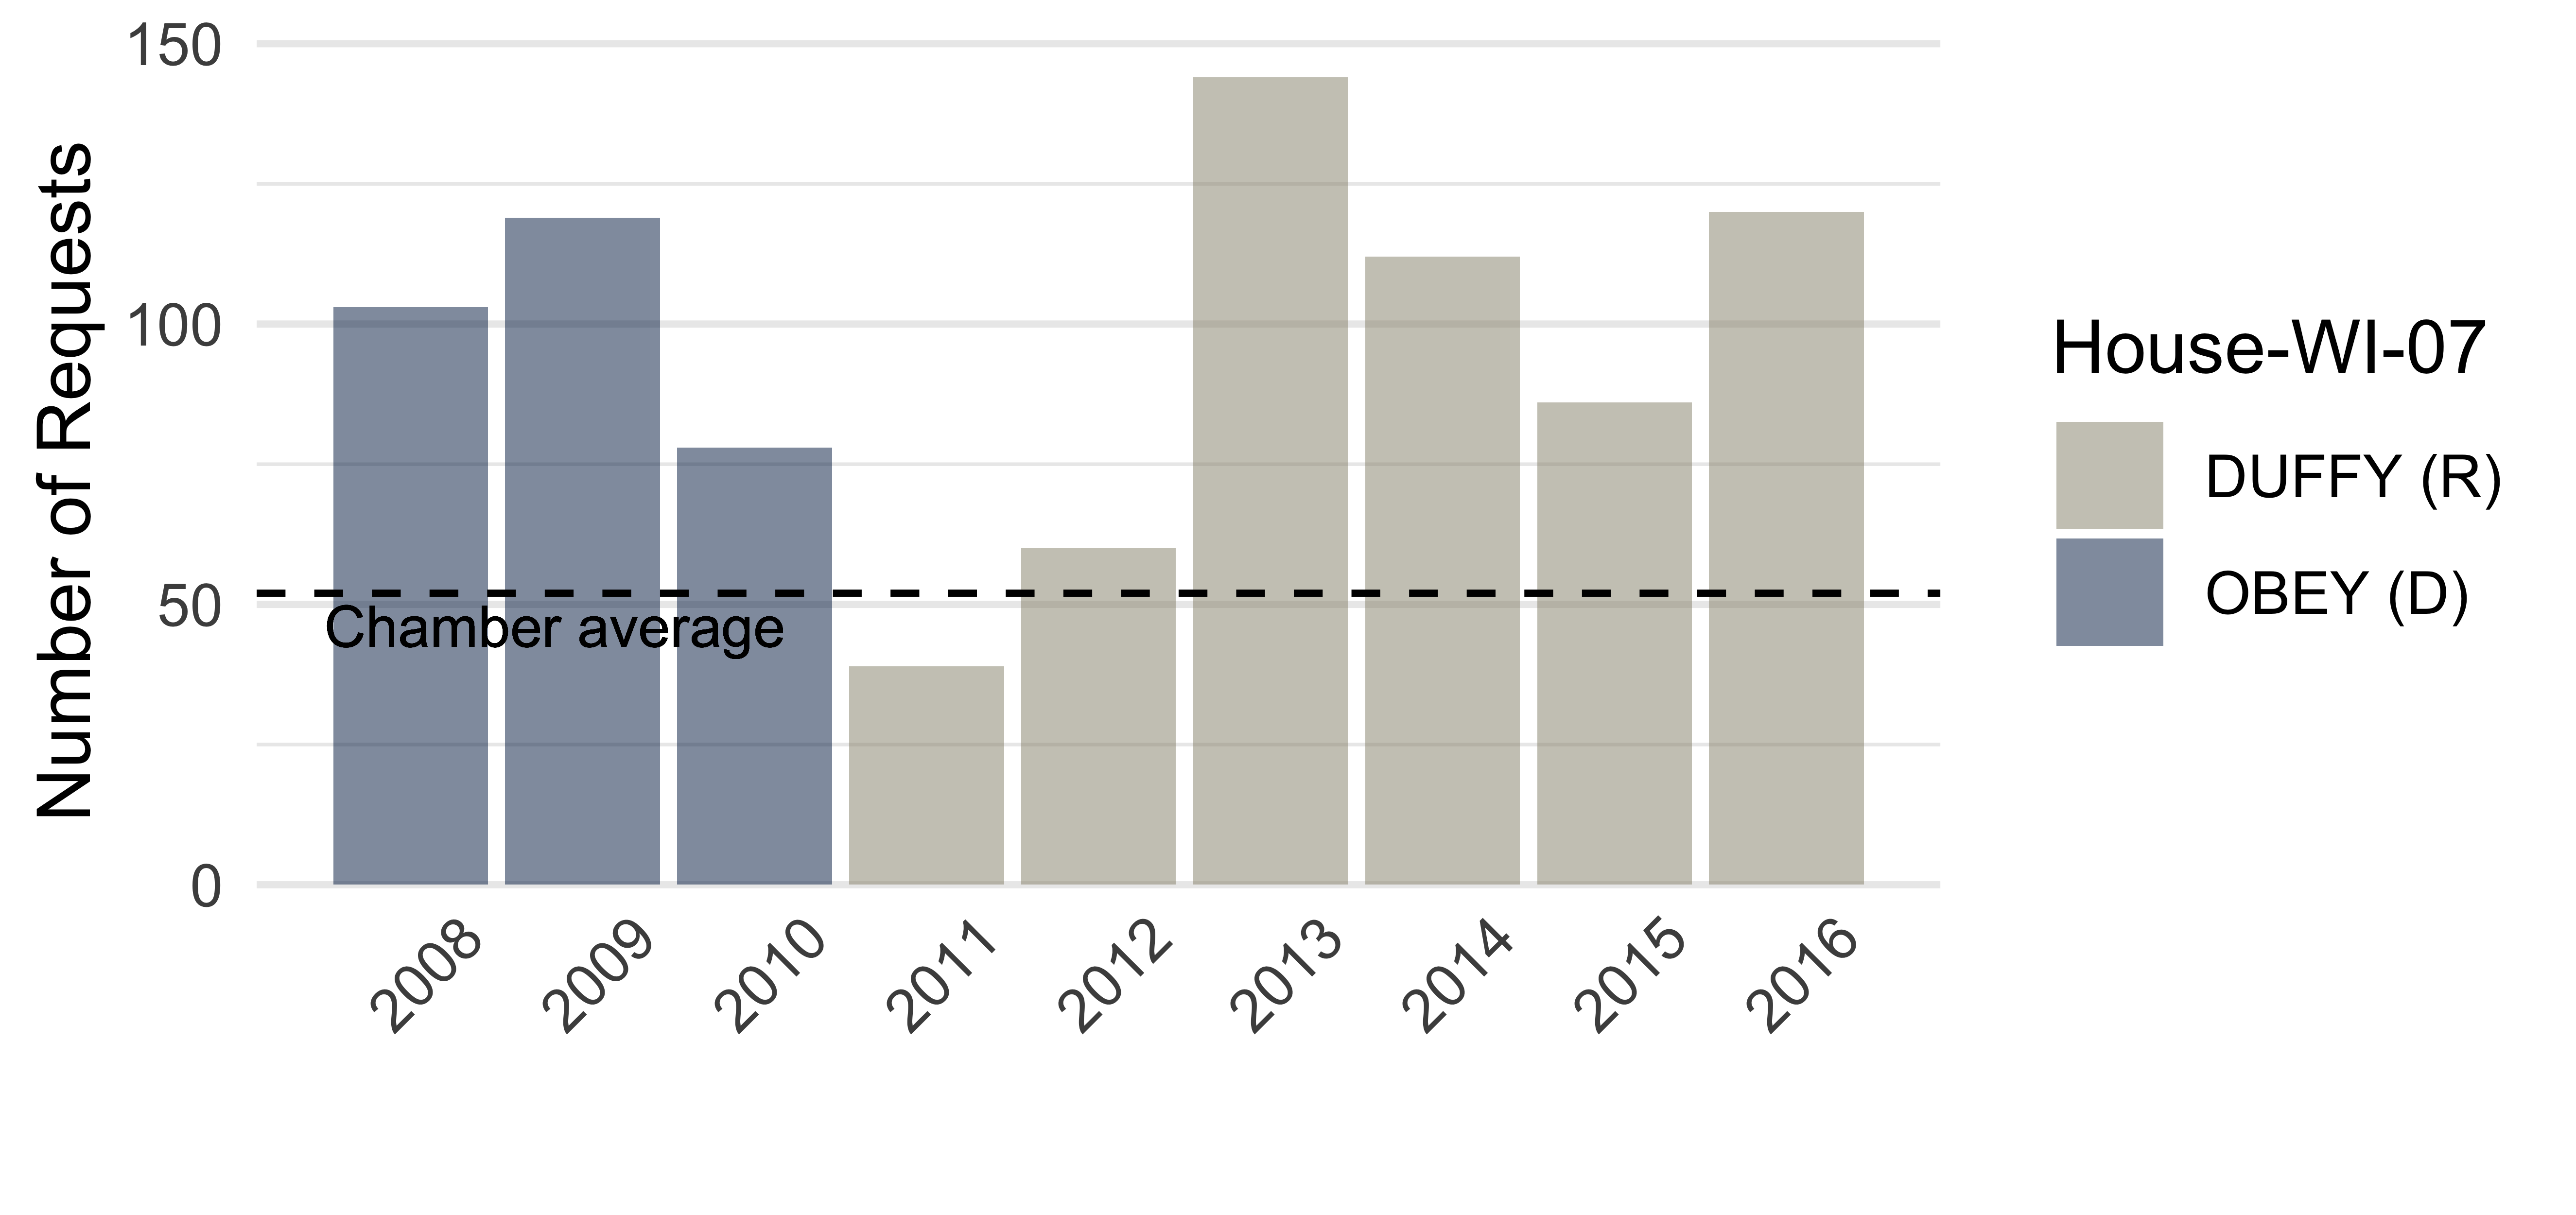
\includegraphics[width = .8\textwidth]{figs/districts/(WI-07)}
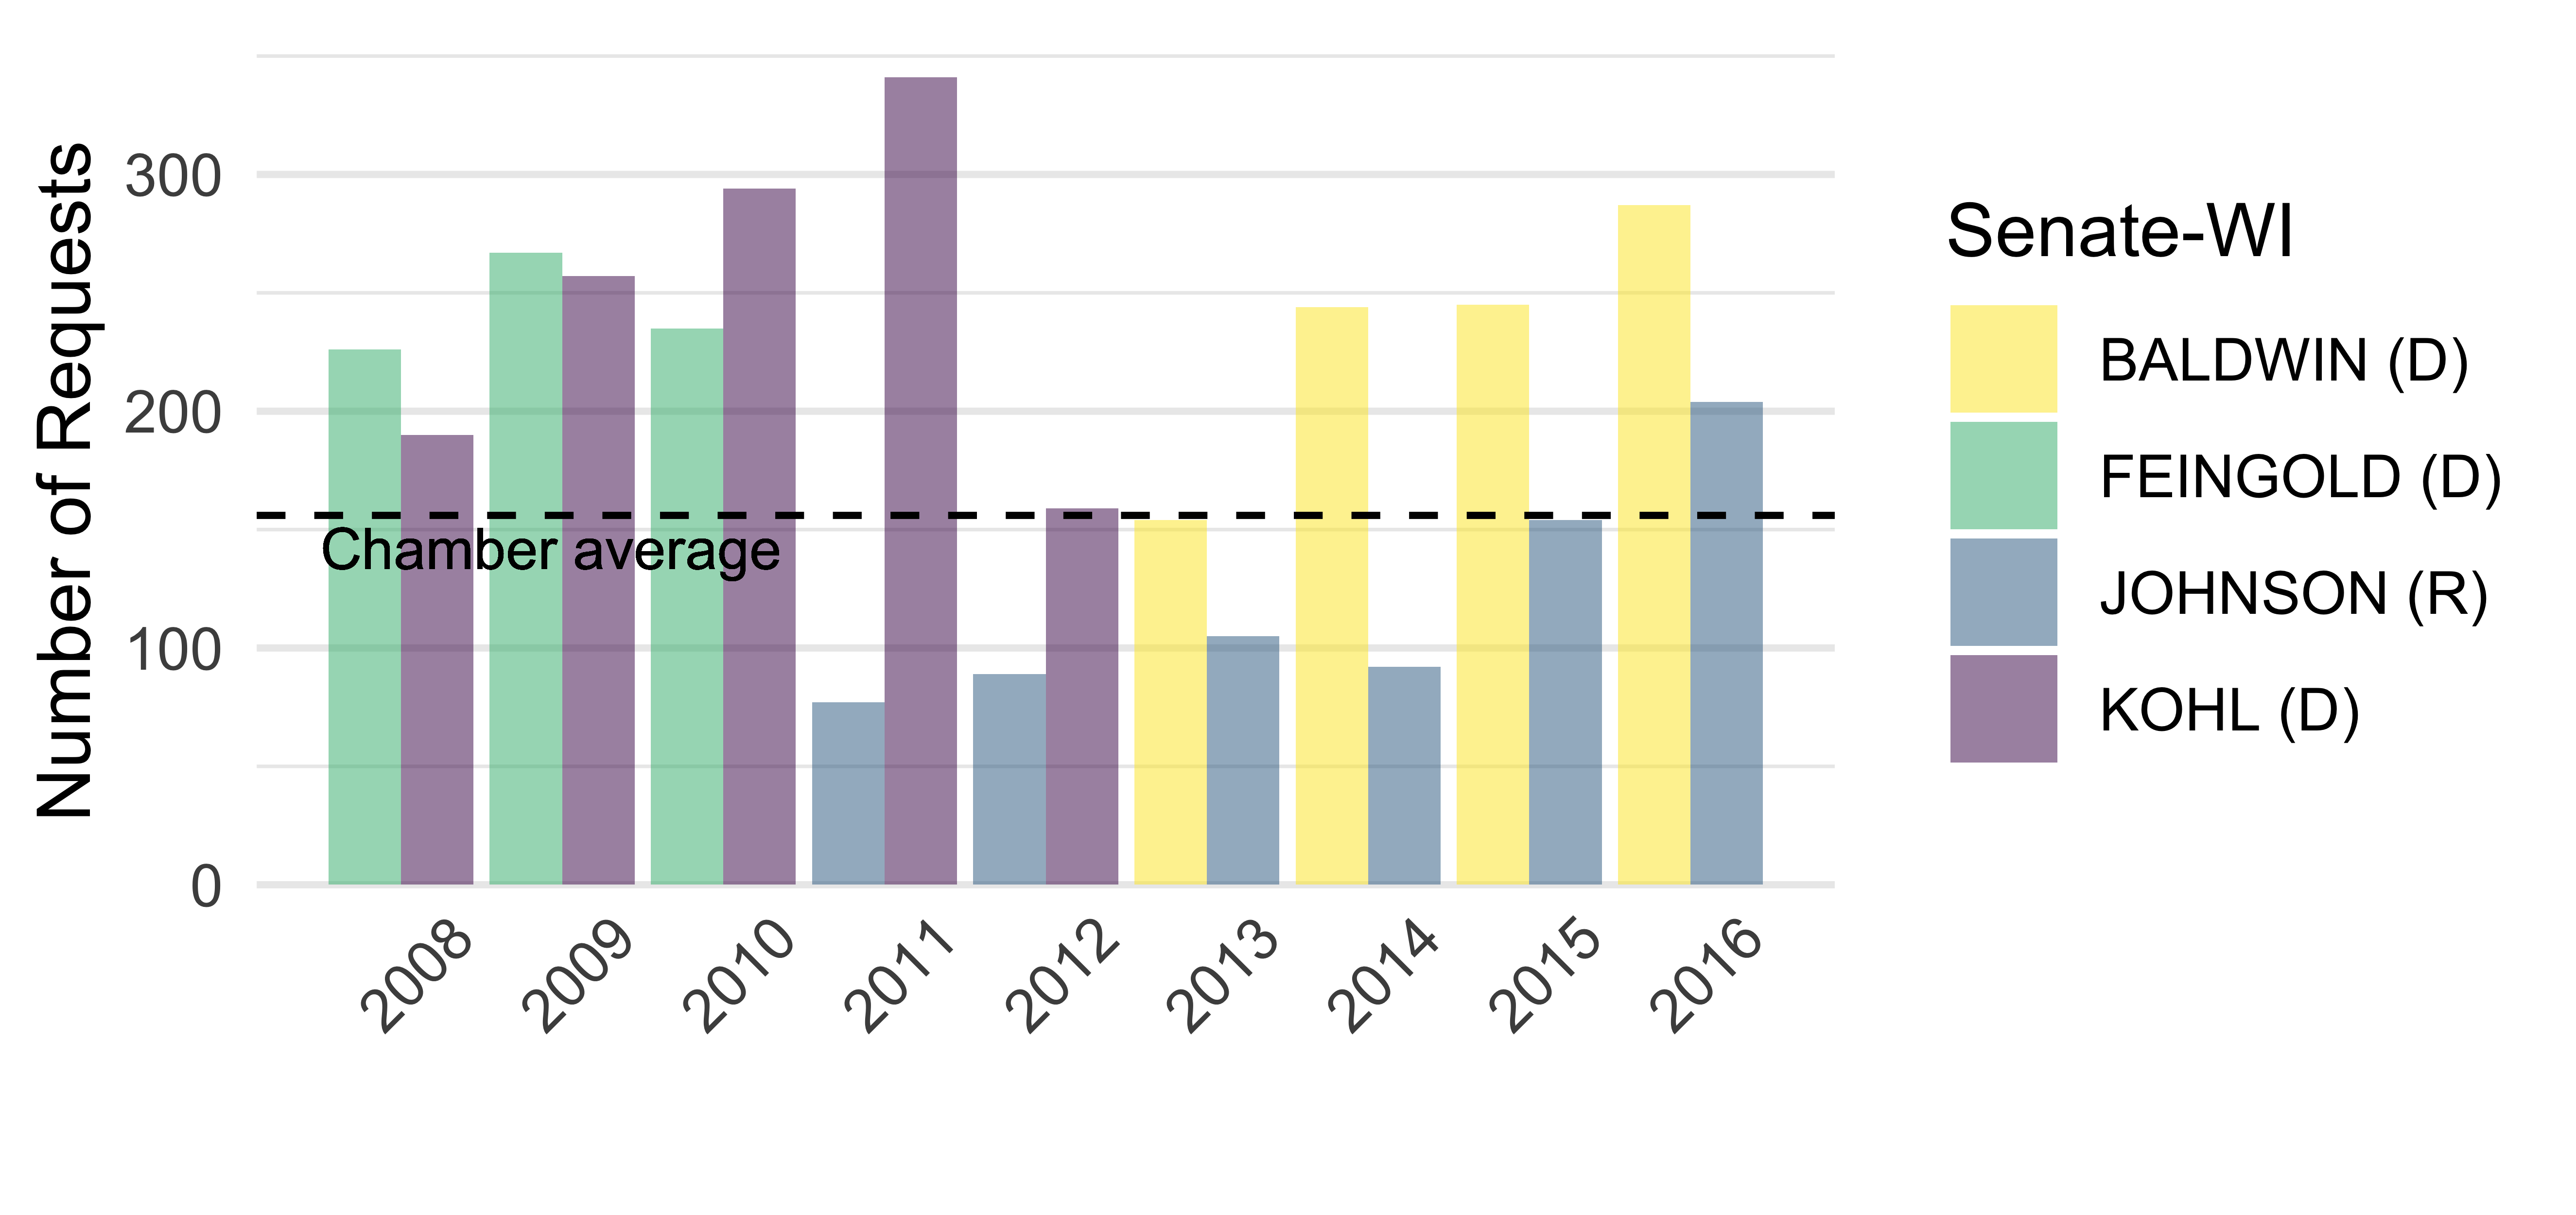
\includegraphics[width = .8\textwidth]{figs/districts/(WI)}
\end{figure}

To make this type of district-level comparison systematically, we change the level of our analysis from the legislator to the district and focus now on the number of contacts made from the representative of a particular state or district $i$ in a year $t$, $Y_{it}$. We again use a difference-in-differences approach to account for district-specific characteristics and over-time changes in how legislators provide constituency service. Specifically, we estimate regressions of the form: 


\begin{eqnarray}
Y_{it} & = & \beta_{1}\text{New Member}_{it} + \sum_{s = 2}^{6} \beta_{s} \text{tenure}_{s[it]} + \gamma_{i} + \delta_{t} + \epsilon_{it} \label{e:district1} 
\end{eqnarray}

$\gamma_{i}$ is a district-specific fixed effect that accounts for each district's particular demographic characteristics, along with the levels of demand from district residents. $\delta_{t}$ is a year fixed effect that controls for common shocks. Our key result of interest, $\beta_{1}$, is the effect of a district electing a new representative. To understand how the effect of a new representative changes over time, we estimate district-level differences for a legislator's second ($\beta_{2}$) through sixth-year ($\beta_{6})$.\footnote{It is worth noting that this treatment is fundamentally different for a district than within-legislator variation. In each election, each district allows its incumbent to acquire another term or replaces her. This differs from within-legislator comparisons because legislators can only acquire more tenure or leave the chamber. A within-legislator analysis estimates the service provided by incumbents with more or less experience; it cannot estimate the impact of the choice of an incumbent or a new representative incumbent.} % TODO THIS FOOTNOTE IS REPETITIVE.

The first column of Table \ref{t:district2} provides a simple difference-in-means for districts represented by a new member and legislators in their first six years in office. Districts represented by new legislators receive substantially lower levels of constituency service. On average, districts with a new representative have 35.2 fewer constituency service requests made on their behalf. The magnitude of this difference shrinks for districts represented by legislators in their second year (23.75 fewer constituency service requests). It then reaches a relatively stable number for districts represented by legislators in their third through sixth years. %, with some slight evidence that legislators make more contacts in election years---the even-numbered years of tenure for the vast majority of legislators in our sample. 



\begin{table}[hbt!]
\caption{The Effect of Electing New Members on a District's Level of Constituency Service} \label{t:district2}
\begin{minipage}{\textwidth}
\begin{center}
\begin{tabular}{l*{4}{c}}
\toprule
                    &\multicolumn{1}{c}{(1)}&\multicolumn{1}{c}{(2)}&\multicolumn{1}{c}{(3)}&\multicolumn{1}{c}{(4)}\\
\midrule
New Legislator      &      -35.23&      -35.55&      -14.89&      -123.5\\
                    &     (4.445)&     (4.500)&     (2.627)&     (13.84)\\
Legislator 2nd Year &      -23.75&      -20.31&      -4.402&      -79.99\\
                    &     (4.464)&     (3.949)&     (2.662)&     (11.34)\\
Legislator 3rd Year &      -13.08&      -13.53&      -1.630&      -49.48\\
                    &     (4.886)&     (4.448)&     (2.586)&     (16.07)\\
Legislator 4th Year &      -12.43&      -9.077&       0.268&      -26.92\\
                    &     (5.216)&     (4.276)&     (2.736)&     (16.30)\\
Legislator 5th Year &      -14.92&      -11.58&      -3.810&      -31.58\\
                    &     (4.416)&     (3.591)&     (2.128)&     (13.11)\\
Legislator 6th Year &      -13.56&      -5.216&      -1.638&      -2.500\\
                    &     (5.104)&     (3.790)&     (2.239)&     (14.46)\\
\midrule
District Fixed Effects&            &  \checkmark&  \checkmark&  \checkmark\\
Year Fixed Effects  &            &  \checkmark&  \checkmark&  \checkmark\\
All Districts       &  \checkmark&  \checkmark&            &            \\
House Only          &            &            &  \checkmark&            \\
Senate Only         &            &            &            &  \checkmark\\
Observations        &        6578&        6578&        5338&        1240\\
\bottomrule
\multicolumn{5}{l}{\footnotesize Robust standard errors in parentheses, clustered at district level}\\
\end{tabular}

\end{center}
\footnotetext{This table shows how constituent service at the district level changes over time. Model 1 is a cross-sectional comparison excluding district and year fixed effects. The second column is a district x year difference in differences model. Column 3 focuses is the diff-in-diff subsetted to legislators who survive their first election.}
\end{minipage}
\end{table}


To account for differences in district size, demographics, and demand for constituency service, the second column of Table \ref{t:district2} estimates the difference-in-differences from Equation \ref{e:district1}. In this specification, we see a large causal effect of a new member taking over: electing a new member causes a decrease of 36 constituency service requests (95-percent confidence interval [-44, -27]), a sizable change in the number of service requests representatives make on behalf of their new constituents. %TODO PERCENT CHANGE 
The effect of electing a new representative, however, dissipates quickly. Districts represented by a legislator in their second year of service receive 12 fewer constituency service requests---still significantly fewer contacts with federal agencies, but not as drastic as the difference observed in the first year. After the second year, the differences are smaller in magnitude. This phenomenon--new legislators providing substantially fewer requests--persists when examining the House (Column 3) and the Senate (Column 4) separately. In short, new legislators make fewer contacts for their constituents than established legislators.  


\paragraph{The Costs of Newly Elected Members} Taken together, our results demonstrate that new legislators provide much less constituency service. Legislators in their first year provide much less constituency service than they do in their second year and reach a stable level of service in their third year. Further, when districts elect a new representative or senator, they experience a sharp decrease in constituency service requests made on their behalf. Rather than experienced legislators forgetting about their districts, our evidence suggests that newly elected legislators experience substantial start-up costs and struggle to provide the levels of service that experienced legislators deliver to their constituents.  


\subsection{The Effect of Experience and Institutional Power on Legislators' Priorities}\label{s:priority} 

To assess legislators' ratio of policy work to constituency service, we use the hand-coded data described in Section \ref{s:data}. The dependent variable in Table \ref{t:models_ratio} is the number of policy requests divided by the number of constituency service requests per legislator per year. These models test whether legislators' priorities shift among goals as they gain experience and power.

\begin{table}
\begin{center}
\begin{minipage}{\textwidth}
\caption{The Effect of Experience and Institutional Power on the Ratio of Policy Work to Constituency Service} \label{t:models_ratio}
\centering
% \begin{tabular}{l*{2}{c}}
\toprule
                    &\multicolumn{1}{c}{(1)}&\multicolumn{1}{c}{(2)}\\
\midrule
Prestige            &      0.0220&     -0.0105\\
                    &   (0.00777)&    (0.0101)\\
Chair               &     -0.0744&     -0.0875\\
                    &    (0.0157)&    (0.0175)\\
Ranking Minority    &    0.000387&     -0.0346\\
                    &    (0.0138)&    (0.0142)\\
First Year          &      0.0428&      0.0223\\
                    &   (0.00918)&    (0.0115)\\
Second Year         &      0.0744&      0.0546\\
                    &   (0.00888)&    (0.0111)\\
Third Year          &      0.0400&      0.0235\\
                    &   (0.00888)&    (0.0107)\\
Fourth Year         &      0.0357&      0.0192\\
                    &   (0.00970)&    (0.0108)\\
Fifth Year          &     0.00801&    -0.00254\\
                    &   (0.00994)&    (0.0105)\\
Sixth Year          &      0.0533&      0.0431\\
                    &   (0.00933)&   (0.00940)\\
\midrule
Majority            &            &  \checkmark\\
Legislator Fixed Effects&            &  \checkmark\\
Year Fixed Effects  &            &  \checkmark\\
Observations        &        6442&        6442\\
\bottomrule
\multicolumn{3}{l}{\footnotesize Robust standard errors in parentheses, clustered at legislator level}\\
\end{tabular}
 % stata version was missing FE
\begin{tabular}[t]{lcc}
\toprule
  & (1) & (2)\\
\midrule
Dependent Variable & Ratio & Ratio\\
\textbf{Committee Chair} & \textbf{\num{-0.070}} & \textbf{\num{-0.071}}\\
\midrule
 & (\num{0.016}) & (\num{0.017})\\
Ranking Member & \num{-0.002} & \num{-0.029}\\
 & (\num{0.013}) & (\num{0.014})\\
Prestige Committee & \num{0.022} & \num{-0.004}\\
 & (\num{0.008}) & (\num{0.009})\\
First Year & \num{0.057} & \num{0.017}\\
 & (\num{0.009}) & (\num{0.014})\\
Second Year & \num{0.064} & \num{0.024}\\
 & (\num{0.008}) & (\num{0.013})\\
Third Year & \num{0.059} & \num{0.021}\\
 & (\num{0.009}) & \vphantom{1} (\num{0.012})\\
Fourth Year & \num{0.035} & \num{-0.003}\\
 & (\num{0.009}) & (\num{0.012})\\
Fifth Year & \num{0.027} & \num{-0.003}\\
 & (\num{0.010}) & (\num{0.011})\\
Sixth Year & \num{0.041} & \num{0.012}\\
 & (\num{0.009}) & (\num{0.010})\\
Majority & \num{0.018} & \num{-0.001}\\
 & (\num{0.006}) & (\num{0.006})\\
President's Party & \num{-0.015} & \num{-0.001}\\
 & (\num{0.005}) & (\num{0.005})\\
\midrule
Observations & \num{6442} & \num{6442}\\
Year Fixed Effects & \checkmark & \checkmark\\
Legislator Fixed Effects &  & \checkmark\\
\bottomrule
\multicolumn{3}{l}{\rule{0pt}{1em}\footnotesize Robust standard errors in parentheses, clustered by legislator.}\\
\end{tabular}
 % this one is from replication.rmd
\footnotetext{This table shows how the proportion of contacts focused on constituency service changes as legislators acquire more experience and power in Congress. Column 1 shows average differences across committee assignments and years in Congress. Column 2 presents difference-in-differences estimates.}
\end{minipage}
\end{center}
\end{table}






Table \ref{t:models_ratio} shows that legislators increase the ratio of policy work to constituency service as they obtain more 
%experience and
prestigious committee assignments. The first column of Table \ref{t:models_ratio} shows how the proportion of policy work to constituency service differs \textit{across} legislators
%in their first six years in office and 
for legislators who acquire committee positions. 

% CAN WE SHORTEN THIS PARAGRAPH? 
While the ratio of policy work to constituency service is conditional on the levels of each, the inference we make about the ratio does not depend on these levels; we are not using the ratio to infer the level (e.g., that a lower share of constituency service means a lower level). Instead, our theory regarding prioritization is about the ratio, regardless of the level. Levels may interact with the ratio, but not in ways that do not mean the same thing for our theory, i.e., legislators prioritize one thing over the other. 

Column 2 of Table \ref{t:models_ratio} provides the estimated effects from the difference-in-differences specification.
We estimate that becoming a committee chair causes the ratio of constituency service to policy work to decrease by 0.08 (95-percent confidence interval [-0.05 , -0.12 ]). Becoming a ranking member of a committee causes a decrease of 0.04 in the ratio.

\begin{figure}[hbt!]
\centering
\caption{Predicted Number of Total Letters (Within Legislator Difference in Differences) 2007-2018} \label{f:m-ratio-predicted}
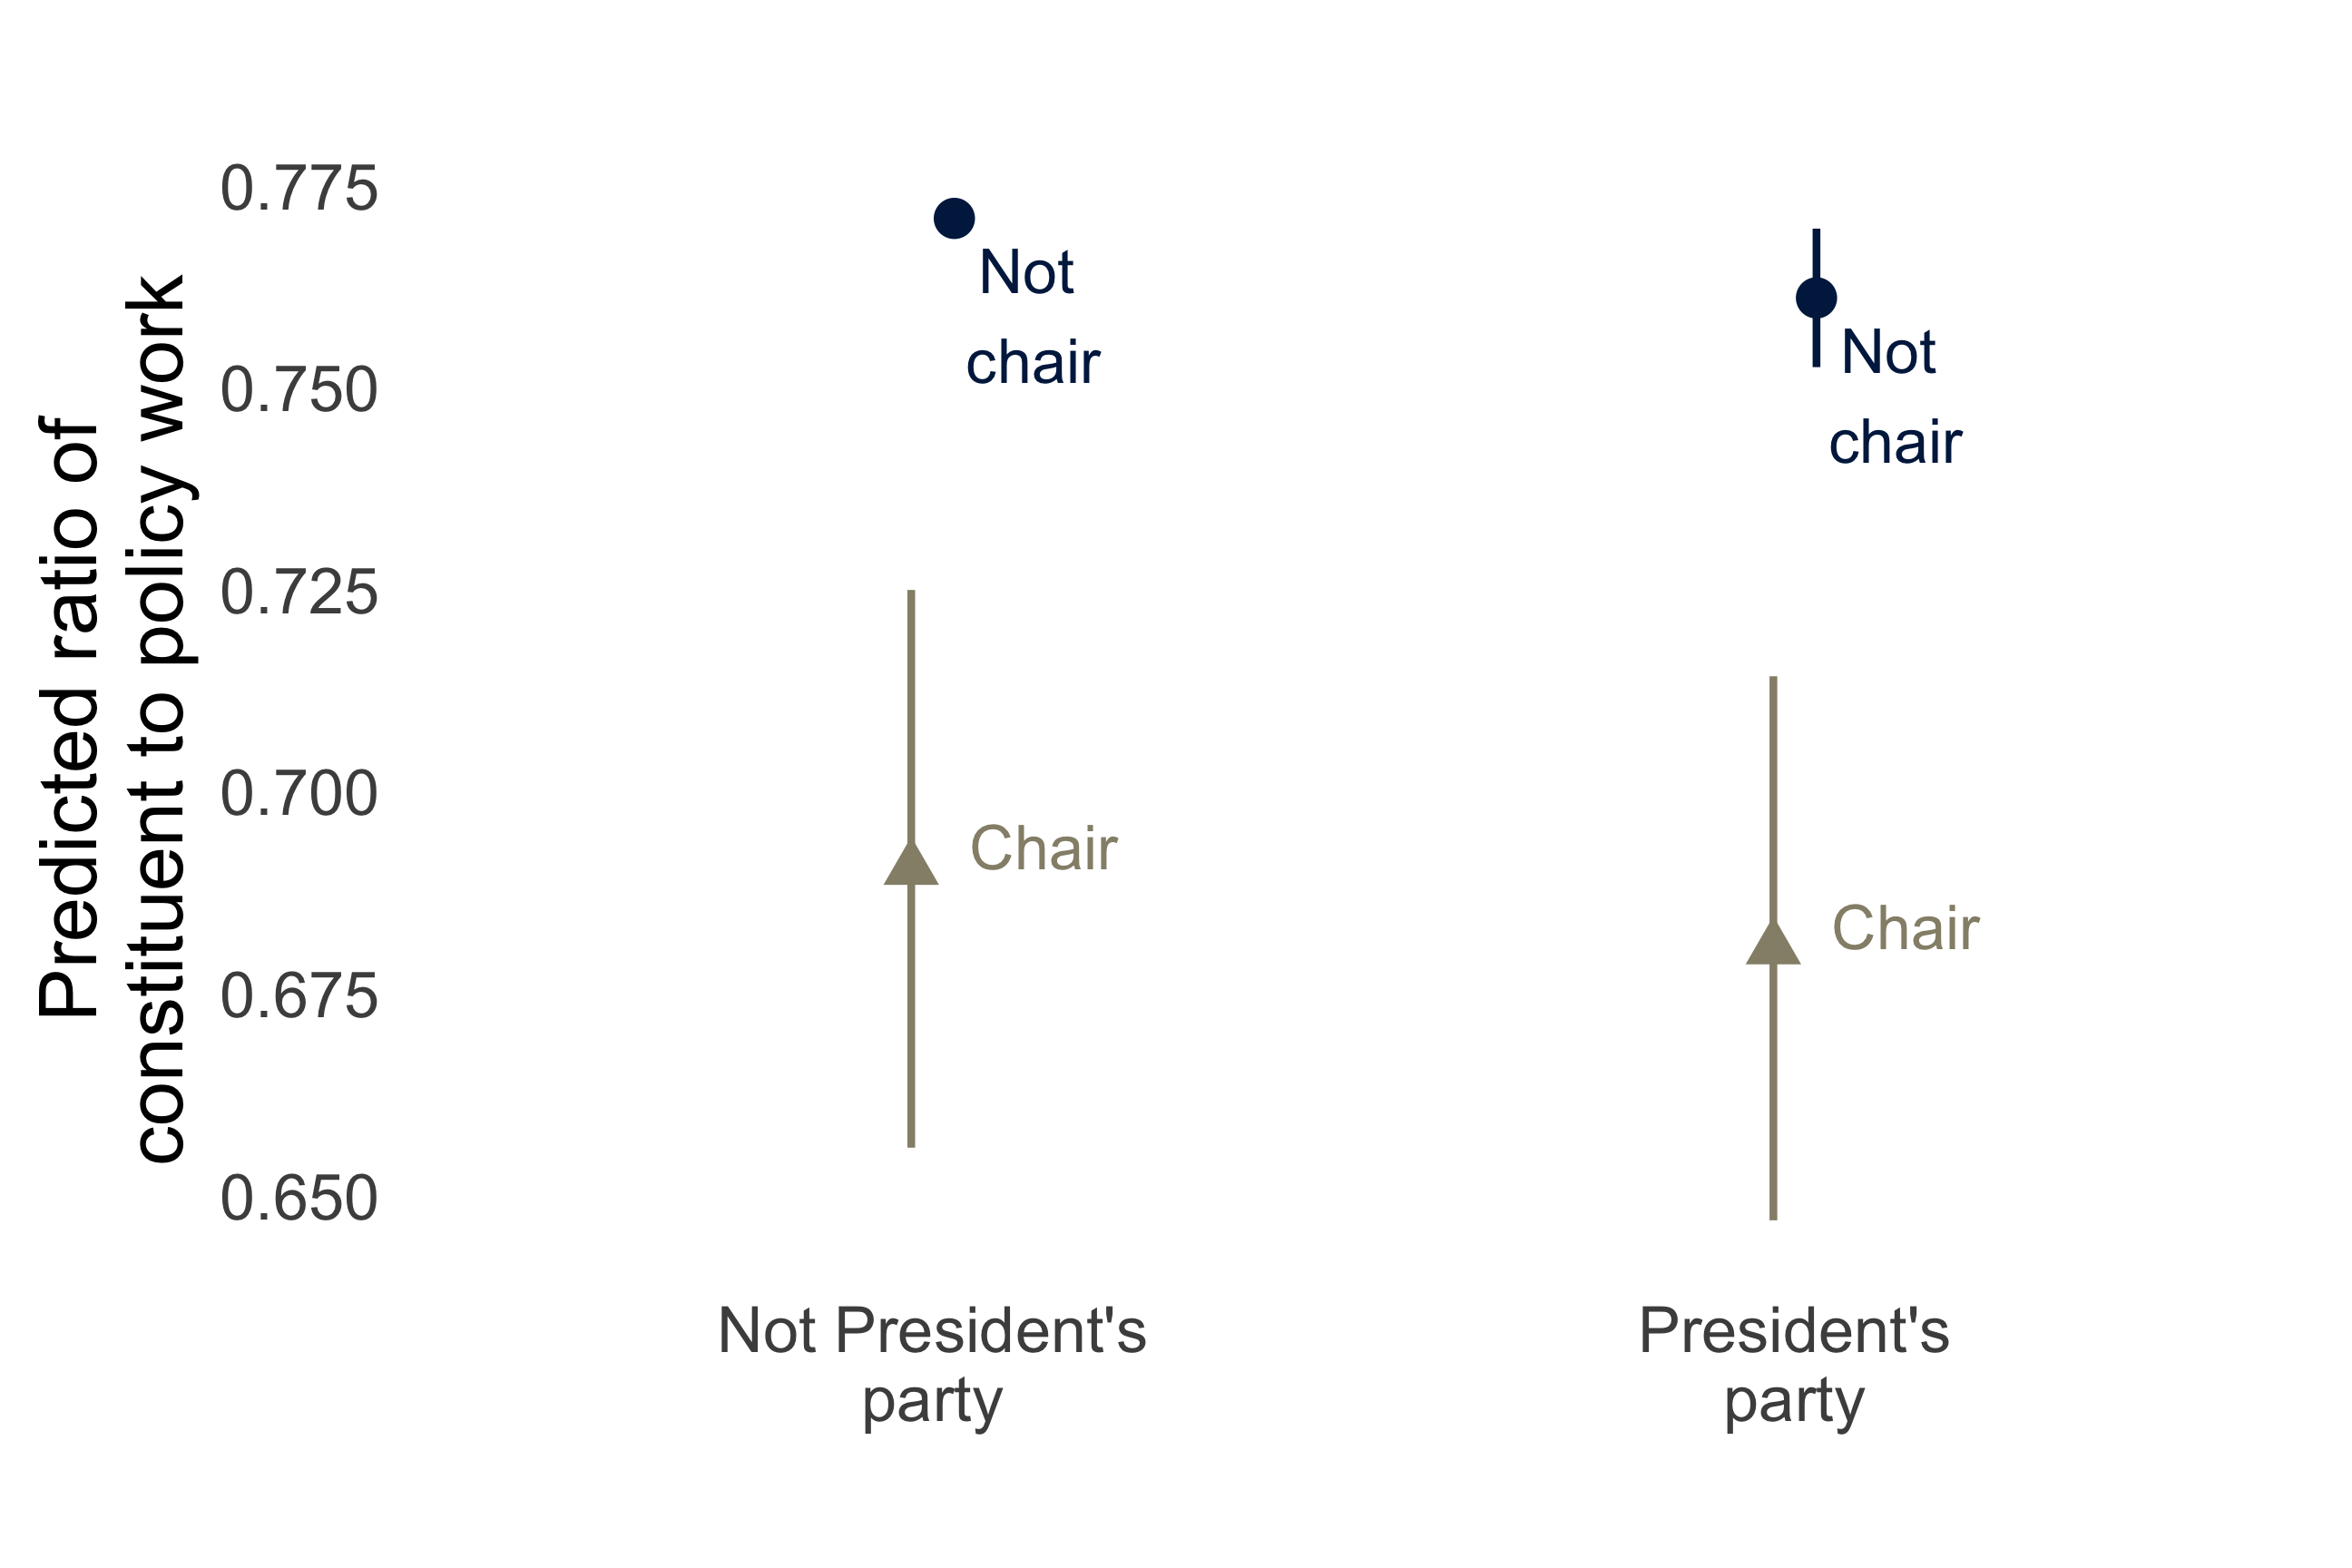
\includegraphics[width = .8\textwidth]{figs/m-ratio-predicted-3}
\end{figure}

Figure \ref{f:m-ratio-predicted} shows the predicted ratio of constituency service to policy work by committee chair status and whether that member has a co-partisan president or not (comparing predictions for counterfactuals where the same legislator did and did not receive a chairship in their sixth year). We estimate chair effects at year six as a plausible year at which a chair position would be acquired. %There is little change in priorities as members gain experience. However, 
There is a significant difference between the same legislator as a committee chair and a counterfactual where they are not. Notably, whether a member has a co-partisan president does not cause a significant difference. 



\section{The Effects of Demand for Constituency Service}\label{s:demand} 

This section shows that demand for constituency service affects the level of constituency service that members provide. However, demand-side shifts do not appear to explain the specific within-legislator or within-district variation we observe with changing committee assignments and increased tenure. %First, we show that constituent demand does drive legislators' constituency service requests to the agencies best suited to address the district's needs. Then, w
We show that this demand does not shift within or across legislators in ways we would expect to see if shifting constituent demand explained the within-legislator and within-district variation in constituency service discussed in section \ref{s:prestigeresults}.

\subsection{District Characteristics Affect the Provision of Constituency Service}

The characteristics of their districts help inform which agencies legislators contact. We find that population size correlates with the overall number of requests and that constituency characteristics—the proportion of veterans and the proportion over 65—correlate with the distribution of requests across agencies. These correlations provide face validity for our measures of representation, but they also suggest that cross-sectional comparisons may conflate legislator choices with district characteristics. Given this potential conflation, our models below include fixed effects for each legislator-agency pair, leveraging within-district and within-agency variation.  

We expect senators who represent larger states to make more requests. Senators from larger states have a larger number of constituents to serve, and they receive a larger budget to handle that increase in requests.
Figure \ref{f:stateSize} shows that this is the case: senators from larger states provide more constituency service on average. Senators from larger states, like John Cornyn (R-TX), Barbara Boxer (D-CA), and Pat Toomey (R-PA), average more requests per year than legislators from smaller states. While the number of legislator requests is associated with population size, Figure \ref{f:stateSize} also shows significant variation in the level of service senators provide, even among states of similar sizes.  

\begin{figure}
\centering
\caption{Average Number of Requests per Senator per Year 2007-2018 by State Population.} \label{f:stateSize}
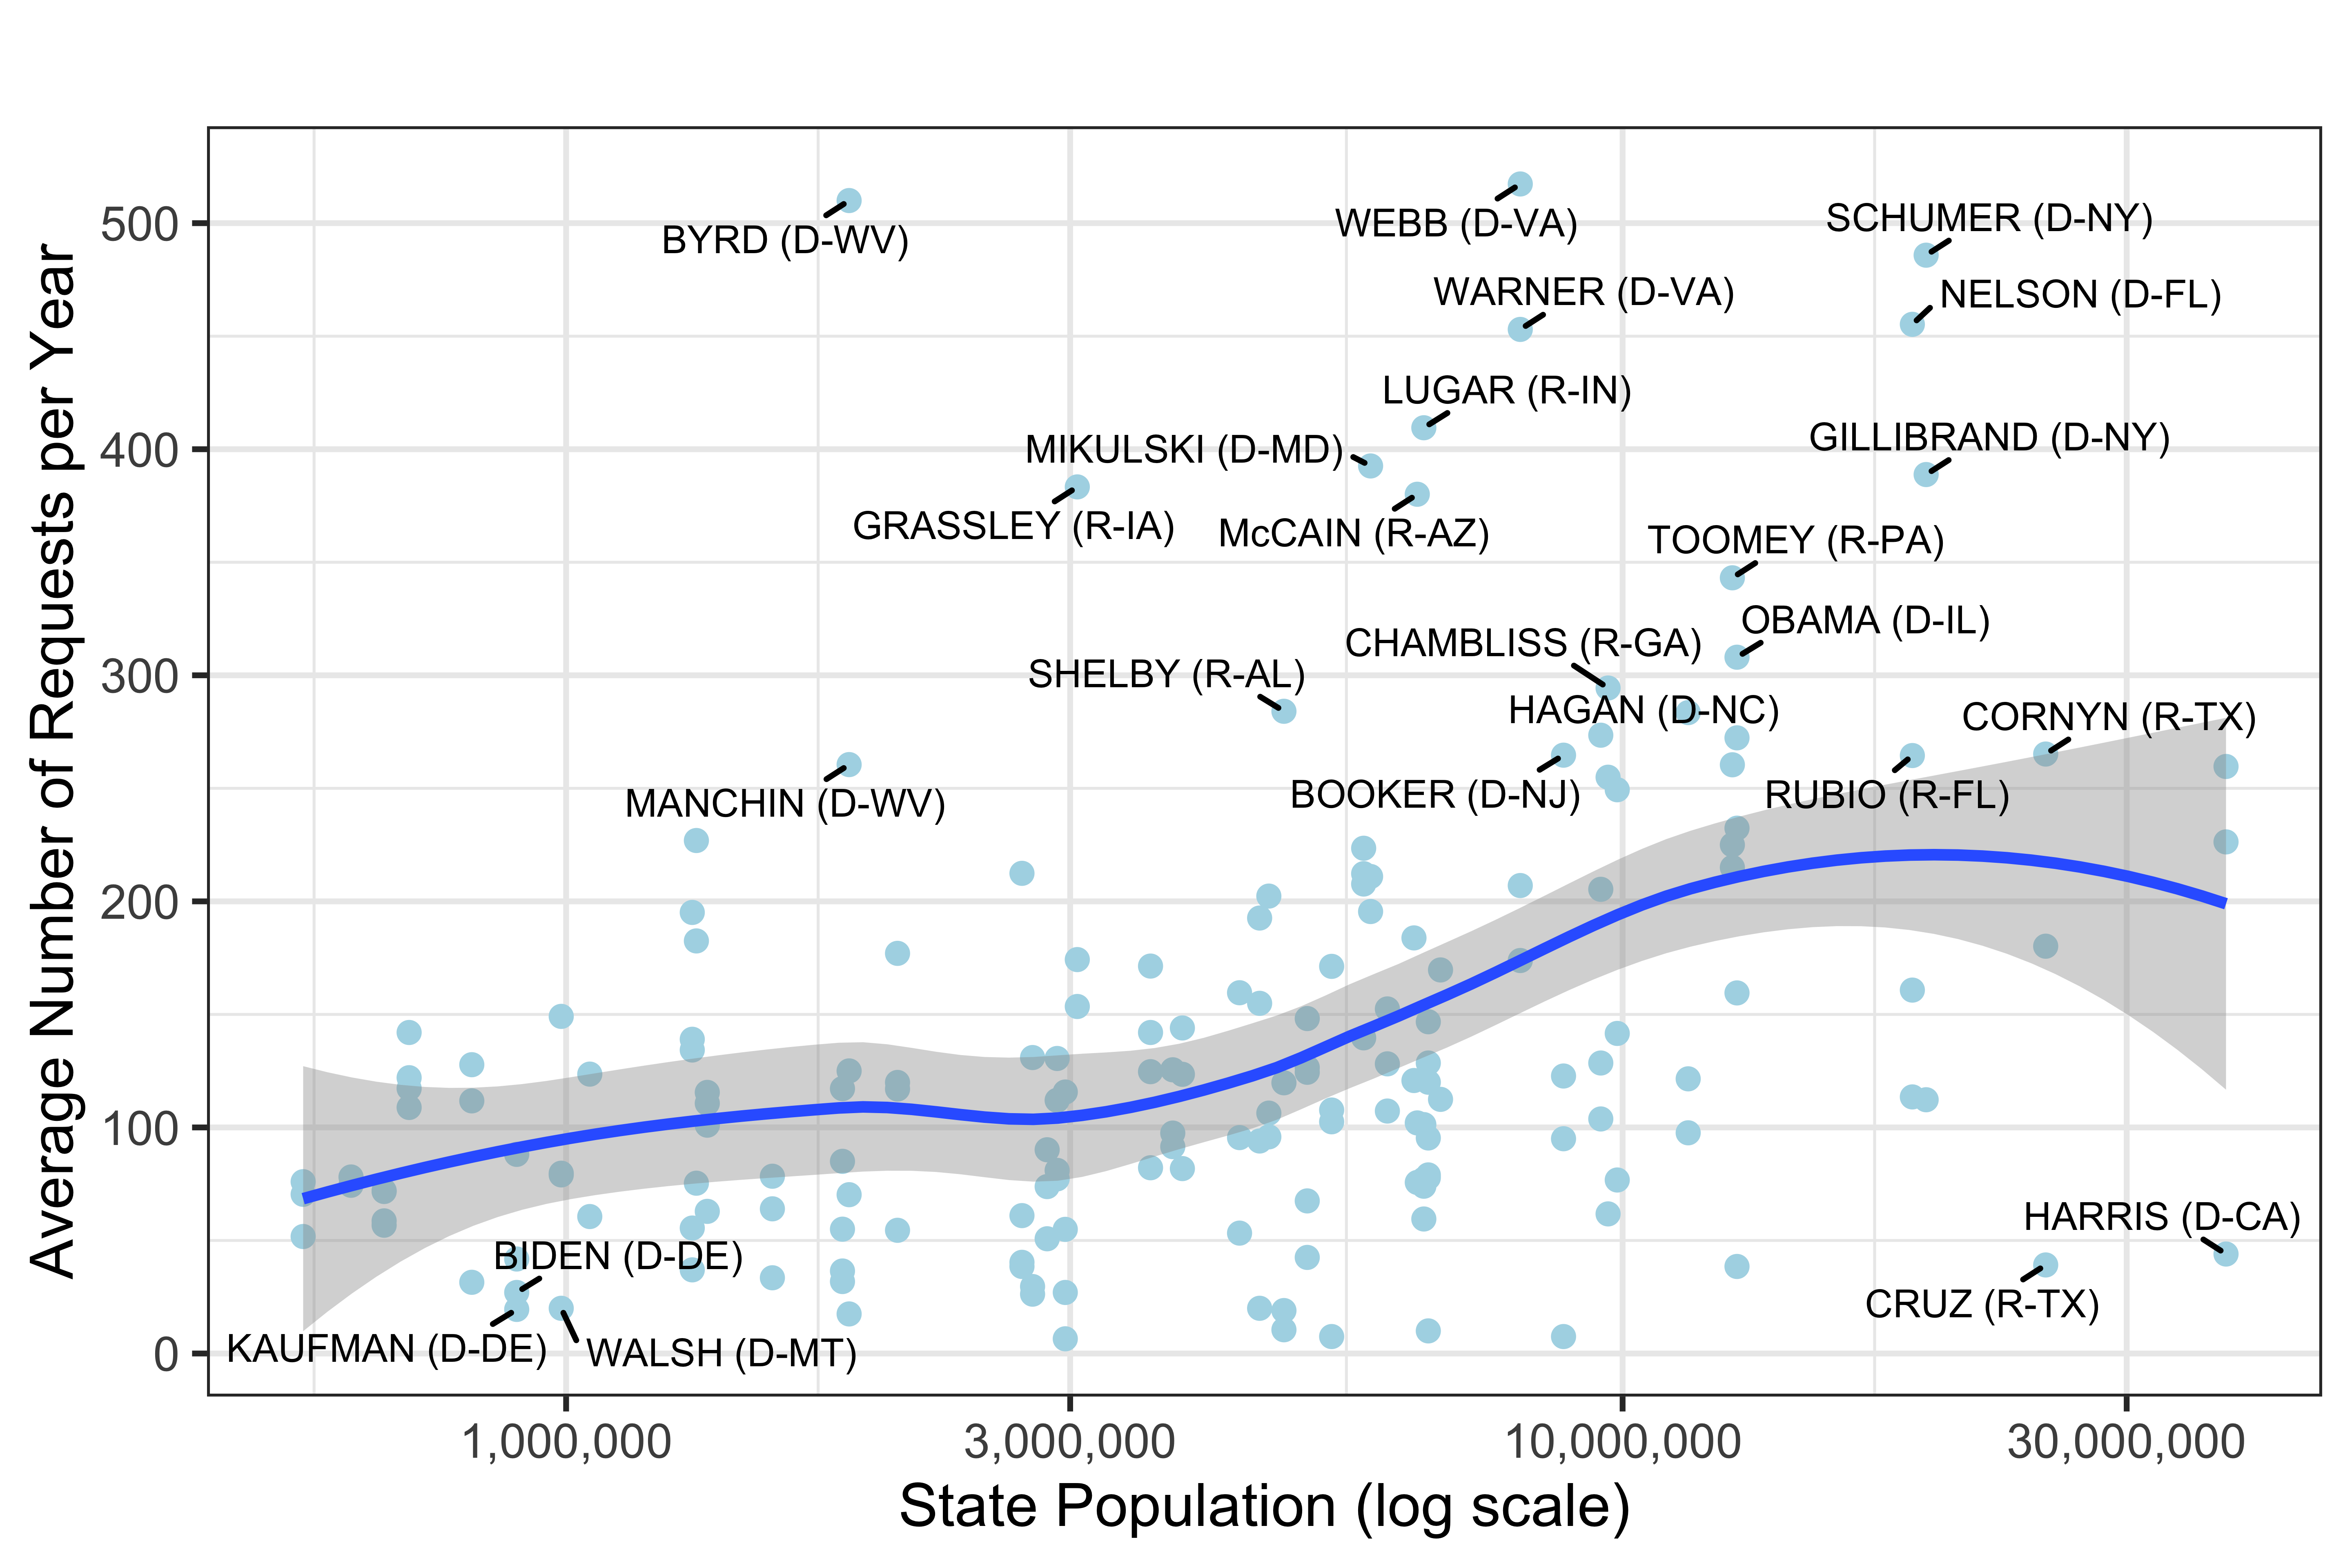
\includegraphics[width = \textwidth]{figs/pop-1}
\end{figure}


%% TODO: REPLACE WITH DESCRIPTIVE FIGURES? 
% We expect the number of times a legislator contacts a particular agency to correlate with their district's demographic composition. To assess the correlation between demographic characteristics and the rates legislators contact agencies, we focus on two example agencies: the Veterans Administration (VA) and the Social Security Administration (SSA). We measured the prevalence of two groups in the district: veterans---the residents who might plausibly need assistance navigating the VA---and residents who are over 65 years of age and therefore satisfy the age eligibility for social security. We then run a simple bivariate regression of the total number of contacts a legislator made to each agency on the proportion of constituents who are veterans or who are over 65.  In both instances, we find a correlation between district composition and the number of times legislators contact the agency. 

%% MOVE THIS TO THE APPENDIX AND ADD THE REGRESSION TABLE
%For example, for the VA, we find that a one percentage point increase in the proportion of residents who are veterans is associated with an increase of about .84 constituency service requests to the agency. Similarly, a one percentage point increase in the proportion of residents over 65 is associated with an increase of an additional 0.03 requests made to the agency. Overall, this suggests that legislators' efforts correlate with the district's demographic composition.  

%% MORE NEEDED HERE

\subsection{Do Voters Demand More of More Powerful Legislators?}

Can variation in demand for constituency service explain why more experience and prestigious committee positions provide more constituency service? 

We limited the influence in demand when assessing how power and experience affect the levels of constituency service above. For example, our empirical strategies in Sections \ref{s:prestige}, \ref{s:tenure}, and \ref{s:priority} account for static demand based on the characteristics of the district. %Districts composed of veterans might see more demand for assistance with the Veterans' Administration, or districts with older residents might have greater demand with the Social Security Administration. 
Because our analyses include either legislator-agency or district fixed effects, we compare how the levels of constituency service change holding constant demand related to fixed district characteristics. Furthermore, %theories of legislator capacity suggest that legislators use their increased capacity and resources to solicit constituency service requests and thus generate demand. %Constituent
demand driven by shifts in legislator behavior is a plausible part of the increased constituency service we attribute to increased capacity and resources.

Yet, we might expect that a legislator's experience or power could affect constituency demand, even without legislators using their increased capacity and resources to generate demand. %, as implied by theories focusing on legislator capacity. 
For example, constituents could direct more of their demands to legislators who are more powerful or who have served longer because they don't know or trust new representatives (holding constant legislators' levels of soliciting constituency service requests). This section investigates whether that additional constituent demand could plausibly explain our results. We find limited effects of legislator tenure on demand for constituency service. 

This section presents a more direct test of whether constituent demand explains variation in legislators' level of constituency service. If constituents shift demand to more experienced legislators, and such a shift could explain levels of constituency service, then we should observe such shifts when a new member is elected. Suppose constituents shift demand based on legislator experience (as required for shifts in demand to explain our results). In that case, they should redirect their demands away from newly elected legislators toward other representatives. The most natural target for the constituent demands would be one of the senators representing the constituent's state.

To assess whether constituents redirect demand toward other more experienced legislators when new members replace their more experienced incumbent representative, we examine how experienced legislators' levels of constituency service change in response to having new representatives in their state. We measure new members in the state in two ways: either the proportion of a state delegation that is new or an indicator of whether there is a new legislator in the delegation. As in Section \ref{s:prestigeresults}, we measure the number of requests a district's representative makes in a particular year. Using this dependent variable, we estimate a series of difference-in-differences regressions where the treatment is new members in the state (Table \ref{t:spill1}). We include district and year fixed effects. We restrict the regression to incumbent legislators only because we are interested in assessing whether constituents with new legislators direct their constituency service requests to these incumbents. 
   
\begin{table}[hbt!]
\caption{No Evidence of Spillovers from New Legislators} \label{t:spill1}

\begin{minipage}{\textwidth}
\begin{center}
\begin{tabular}{l*{4}{c}}
\toprule
                    &\multicolumn{1}{c}{(1)}&\multicolumn{1}{c}{(2)}&\multicolumn{1}{c}{(3)}&\multicolumn{1}{c}{(4)}\\
\midrule
Proportion New Legislators&       5.143&            &      -1.494&            \\
                    &     (8.089)&            &     (20.06)&            \\
At Least One New Legislator&            &       1.625&            &       3.847\\
                    &            &     (2.031)&            &     (4.812)\\
\midrule
District Fixed Effects&  \checkmark&  \checkmark&  \checkmark&  \checkmark\\
Year Fixed Effects  &  \checkmark&  \checkmark&  \checkmark&  \checkmark\\
Senators Only       &            &            &  \checkmark&  \checkmark\\
Observations        &        6080&        6080&        1182&        1182\\
\bottomrule
\multicolumn{5}{l}{\footnotesize Robust standard errors in parentheses, clustered at district level}\\
\end{tabular}

\end{center}
\end{minipage}
\end{table}

The first two columns of Table \ref{t:spill1} are estimates for all incumbent legislators, and they show that neither the proportion of new members nor a new member significantly affects the level of constituency service that other legislators in the state provide. Columns 3 and 4 of Table \ref{t:spill1} reveal the same pattern when focusing on senators only. Across all four specifications, the estimated effects of new legislators do not approach statistical significance.  This consistent null finding regarding the impact of new legislators in a state delegation provides reassurance that there's little (to no) evidence of constituents redirecting demand toward other, more experienced legislators in response to having new representatives in their state delegation. %%% Note: Ellie stopped here. 




\section{Discussion} \label{s:discussion}

%% 1 Summary of findings

%% 2  Implications for theory (evidence that capacity matters, evidence that priorities change, the importance of studying both at the same time)

%% 3  Implications for policy (term limits, congressional staff, anything else)

%% 4 Future research (things one can do with these data; cite our other stuff, what else?) 


%% SUMMARY OF FINDINGS - MOVE TO CONCLUSION?
Most legislator contacts with federal agencies focus on constituency service. While there is massive inequality in the quantity of service provided by different members, we show that this is not the result of long-serving members devoting less attention to their district over time, as the ``Potomac Fever'' hypothesis suggests. We find evidence that legislators prioritize policy work as they acquire positions of institutional power. However, simultaneous increases in capacity that come with positions of institutional power more than offset shifting priorities. Critically, the magnitude of the effect of increased capacity is large enough that the district constituency receives no less particularistic service from long-serving and powerful legislators. 

%Using a robust research design that includes both cross-sectional and within-legislator variation, we show that...
%In Section \ref{s:prestige}, we showed that legislators provide more constituency service as they gain experience. In Section \ref{s:priority}, we showed that legislators also increase their ratio of policy work to constituency service when they gain experience and power. These latter two findings have potentially countervailing effects on the overall level of constituency service (accounting for simultaneous shifts in capacity and priority). The key outcome is the net effect on levels of constituency service, accounting for the effects of both increasing capacity on the level of constituency service (Table \ref{t:models_total}) and shifting priorities on the ratio of policy work to constituency service (Table \ref{t:models_ratio}). 

%% IMPLICATIONS FOR THEORY 
\subsection{Implications for Theory}

% SIMULTANEOUS EFFECTS 
Our finding that shifts in capacity and priorities simultaneously affect contacts with agencies implies that scholars of legislator behavior should focus both on the levels of effort legislators provide and how they divide that effort. Legislator requests to the bureaucracy are one of many types of behavior that are likely affected by simultaneous changes in capacity and priority. In addition to correspondence with federal agencies, the volume of legislative work, oversight reports, or hearings produced by a legislator's office depends both on their capacity to do that work and the relative priority of each task. %Research designs that aim to identify the cause of any increased productivity as elected officials gain experience or achieve a position of institutional power must be able to tell whether the outcome resulted from shifting capacity, shifting priorities, or some combination of both. 

%MECHANISMS 
Further, our findings suggest that the mechanisms we identify---organizational efficiency, office resources, and likelihood of success---help explain legislator behavior. The dramatic decrease in requests when new legislators take office is consistent with the organizational efficiency mechanism. Becoming a committee chair increases the resources available to a legislator and their volume of contact with federal agencies. Both results are consistent with legislators making more requests to federal agencies when they are likely to perceive greater rewards.

%Furthermore, we find evidence for multiple mechanisms contributing to increased capacity's overall effect. We find that legislator experience matters. The volume of legislator requests to the bureaucracy increases dramatically in the first few years, well before legislators generally acquire committee chairmanships or other positions of institutional power that come with additional staff resources. This large, short-lived effect of being a new legislator is evidence for the Organizational Efficiency mechanism we theorize. Because new legislators rarely become committee chairs, the large effect of gaining a committee chair position is evidence for the Increased Likelihood of Success mechanism that we theorize. 

% CONSTITUENCY SERVICE DESERVES ATTENTION 
The fact that elected officials continue to dedicate substantial resources to constituency service well into their careers and after they have achieved high-status institutional positions is evidence that constituency services is a core function of congressional offices. This calls for renewed attention to the motivations for and effects of constituency service in modern U.S. democracy. As we collected and coded these data, we spoke to numerous staffers and agency officials. A recurring theme in the data and stories we heard was the interaction between constituency service casework and other activities, including oversight investigations and legislation. Conversely, new legislation often resulted in new forms of constituency service as legislators helped their constituents attain newly legislated benefits, deal with new paperwork requirements, or avoid new regulatory requirements. While constituency service may have underlying electoral motivations, as formal models suggest, it is also a prominent yet understudied form of legislator behavior in its own right. 

% REPRESENTATION 
Our finding that experience and institutional power allow legislators to do more policy work while maintaining levels of constituent service complements recent scholarship on representation. The same legislators who \citet{Grose2011}, 
%\citet{Butler2011}, \citet{Broockman2013}, \citet{Butler2014}, 
\citet{Dinesen2021}, 
\citet{LowandeRitchieLauterbach2018}, 
and others find doing more casework for minority groups also likely to do more policy work on behalf of those groups (in line with \citet{Mendez2018}) and higher rates of advocacy for nonprofits that serve those groups. While legislators must prioritize limited time \citep{Kaslovsky2022}, institutional power adds to the capacity of a legislative office as an institution to pursue both policy work and constituency service. Because institutional power comes with resources, representation matters not just in Congress but also in powerful positions like committee chairs. 
%% Devin: I re-read Mansbridge and decided that her categories (surprisingly) don't fit too neatly. Policy work is both promissory and anticipatory. Constituency service is also anticipatory and occasionally surrogate (surrogate is a very good term for constituency service, but Mansbridge defines it as representing people not in your district). I left it out for now unless you see a sensible way to say it. 

% INCUMBENCY ADVANTAGE 
%Our results also offer a rationale for the incumbency advantage: when constituents choose between legislators, replacing an incumbent legislator comes at the cost of less constituency service and policy work. Incumbents who have acquired experience and power in Washington are most able to deliver service to their constituents in the next legislative term.    

%% 2  Implications for policy (term limits, congressional staff, anything else)
\subsection{Implications for Policy}

% POTENTIAL IMPACT OF STAFF 
The large effects of legislator capacity that we find add to a recent wave of scholarship on the impact of congressional staffing. \citet{LaPira2020} document many effects that decreasing staffing levels may have on the functioning of Congress. Because increased staff for committee chairs is a likely mechanism for the capacity effects we find, our results offer a key outcome measure and effect sizes that may correspond to additional staff.  
While committee chairs simultaneously obtain other forms of power like agenda control, to the extent that our results reflect the capacity boost of committee staff, 
our evidence suggests that congressional staff likely have measurable and potentially large effects on the volume of work legislators can do. 
% Our data also provide a measure of the effect of staff allocation https://static1.squarespace.com/static/59e25521b7411c07ef1410fa/t/5d0a8942790f8e00019661cb/1560971588406/comp_ideo_full_62019.pdf

% TERM LIMITS 
Advocates for term limits often argue that elected officials lose touch with their district. In contrast, we show that more experienced legislators provide as much or more service to their district, even as they do more policy work. Moreover, our results show that new legislators have less capacity to make requests to federal agencies. Removing experienced legislators would likely decrease levels of constituency service. 


%% 3 Future research (cite our other stuff, what else?) 

\subsection{Future Research}

Future research should further examine the mechanisms by which increasing experience and capacity shape legislator behavior. This could include explicit measures of office organization and efficiency and more nuanced measures of institutional power. This could also include measuring agency responsiveness to legislator requests. Likewise, future research could examine mechanisms related to shifting priorities. Finally, future work could include legislators' substantive areas of expertise. Does expertise increase a legislator's capacity to act in certain areas (e.g., certain agencies), leading to more capacity for constituency service? Does increased institutional power lead legislators to develop expertise, for example, in certain committee work or specialized policy work that builds their capacity to influence certain agencies? 

The massive new dataset we introduce here will help scholars answer these questions. With data from nearly all parts of the vast U.S. federal bureaucracy, future work can advance the study of descriptive representation, expanding on work by \citet{LowandeRitchieLauterbach2018}, who find that women, minority, and veteran members do more casework on behalf of groups that share their identity. The new data we collect will allow similar tests of representation for other demographic groups, including seniors, farmers, and low-income populations, to name just a few. Likewise, more data will allow new tests of prior work showing that members use lobbying the bureaucracy to advance policy goals when they conflict with their party's agenda \citep{Ritchie2017}. Our systematic data allow tests of variation across policy domains and government functions. 

Critically, our systematic approach to data collection allows more general tests of legislator behavior. Any sample focusing on a few policy domains or agencies will over-represent legislators sitting on certain oversight committees and representing certain constituencies. Our near-census of legislator contacts minimizes such confounders and will allow researchers to test more general theories of legislator behavior, as we have done here.

\section{Conclusion} \label{s:conclude}

%Shifting priorities—the change in the ratio of policy work to constituency service—do not overpower the effects of increased capacity and power—the change in the overall number of requests to federal agencies, with even more powerful legislators focusing primarily on constituency service. 
%Using a new data set on legislators' requests made to federal agencies, we show that, 
As legislators gain experience and power, they both gain the capacity to make more requests to agencies while simultaneously shifting priorities to policy work. Crucially, the increase in capacity is large enough relative to the shift in attention toward policy work that legislators maintain or even increase levels of constituency service as they gain institutional power. Consistent with our theory that experience increases capacity, we also show that legislators make fewer service requests at the start of their careers and that new legislators make substantially fewer service requests than their more experienced colleagues. 

%Theories that assert that capacity matters correctly predict that the levels of both constituency service and policy work increase as legislators gain experience and institutional power in Congress.
%Theories asserting that legislators shift priorities correctly predict that the ratio of policy work to constituency service increases as legislators spend more time and gain institutional power in Congress.
%Empirically, the net result of both effects is a net increase in policy work and constituency service levels as legislators spend more time and gain institutional power in Congress; there is no trade-off.

%Taken together, our findings show that the reelection motivation remains a potent force for even the most powerful legislators in Washington. Rather than use increased power in the institution as an excuse to be less attentive to the district or increased time in Washington to be less interested in their constituencies, our results show that legislators with more power and experience provide no less constituency service to their district, even as they increase their attention to policy work. 

%TODO BETTER CONCLUSION
%Rather than forgetting about the district and contracting Potomac Fever, it appears that more experience and power in Congress enables legislators to deliver particular goods to the district more effectively.  

\singlespacing

\bibliography{congress2019}

\clearpage
\appendix
\setcounter{table}{0}
\renewcommand{\thetable}{A\arabic{table}}



\section*{Appendix}


\section{FOIA Data}

Our data represent a near census of requests to federal departments, agencies, and sub-agencies. We received records from every department other than the Department of State,\footnote{The Department of State has a notorious FOIA backlog of approximately 10,500 cases. The FOIA office expects to fill our May 2018 request in 2024.} 
and most independent agencies, commissions, boards, executive offices (e.g., the Council on Environmental Quality and U.S. Trade Representative), and pseudo-governmental institutions like Amtrak and the US Export-Import Bank. 

\paragraph{Variation in Responses to Identical FOIA Request} Responses to our FOIA requests varied significantly. Most agencies offered logs of congressional correspondence, which record a date, sender, summary of the request, and other information used by agency staff to process and respond to requests. Logs generally include any written requests, as well as many phone and email records. For example, between May 2015 and December 2017, the Department of Justice Office of Administrative Law Judges received 132 emails, 109 telephone calls, and only 54 letters. Between 2007 and 2017, the Postal Regulatory Commission received 100 emails, 30 faxes, 173 letters, and 118 calls. In this paper, we use ``contacts'' and ``letters'' interchangeably to refer to all modes of correspondence. 

Small agencies and regional offices had staff search their email history or provided hand-written records, which we then transcribed. Department Secretary offices generally queried a correspondence tracking database designed to track all correspondence. Still, our FOIA requests to sub-departmental components almost always recovered additional congressional correspondence records missing from central databases. As one central office FOIA officer put it, ``Legislative Affairs is supposed to be the front door for the department, but if somebody knows somebody, well...'' (personal communication, February 21, 2018). Because of such idiosyncratic relationships, capturing correspondence patterns that ``go around'' a Department Secretary's office is key to avoiding erroneous inferences about legislator behavior. For example, when chairs of the Homeland Security committee wrote about immigration enforcement issues, they almost always contacted the Department of Homeland Security (DHS) office of the Executive Secretary, but, at the same time, the Immigration Customs Enforcement (ICE) component of DHS directly received thousands of requests from a different set of legislators. Our systematic data collection ensures that we capture the totality of legislators' behavior.

%%% Ellie: I manually changed the input code here to fit the entire table.  
%\input{tables/FOIA_response.tex}

% TODO replace with this one generated by Appendix.rmd when I get the formatting right

\begin{tabular}{lrrr}
\toprule
Department & Components FOIAed & Records received & N\\
\midrule
Agriculture & 29 & 29 & 9516\\
Commerce & 19 & 18 & 8038\\
Defense & 49 & 13 & 9739\\
Education & 1 & 1 & 4689\\
Energy & 8 & 2 & 6580\\
\addlinespace
Health and Human Services & 15 & 10 & 104145\\
Homeland Security & 14 & 13 & 39633\\
Housing and Urban Development & 2 & 1 & 33968\\
Justice & 23 & 5 & 2611\\
Labor & 22 & 12 & 53341\\
\addlinespace
State & 1 & 0 & 0\\
the Interior & 11 & 8 & 6079\\
the Treasury & 7 & 5 & 23869\\
Transportation & 10 & 7 & 26787\\
Veterans Affairs & 6 & 3 & 77842\\
\addlinespace
Independent Agencies & 77 & 47 & 81053\\
\midrule
\textbf{Total} & \textbf{294} & \textbf{174} & \textbf{487890}\\
\bottomrule
\end{tabular}



\section{Contact Codebook} \label{a:codebook}
\singlespacing
%%% Note: From Ellie. I deleted everything here that we're not using in this paper.  

We provide the following codebook to a team of hand-coders to code each case of Congressional contact with federal agencies and extract information about the legislator. The codebook provides steps to move from raw correspondence logs to data formatted for our analysis.  We also developed subagency-specific coding rules throughout the hand-coding process where certain regular expressions indicated certain types of requests. For example, where documents containing the word ``rulemaking" consistently indicated that a legislator's request involved an agency's proposed rule, we assigned all observations containing the word ``rulemaking" yet uncoded by hand to the ``Policy-Rulemaking" category.\footnote{Hundreds of scripts for processing the raw data from each agency and applying any inductively-generated regular-expression-based coding are available on our GitHub, along with each script's full revision history and all written communication with RAs about processing and coding these data.}

We classify legislator requests into five categories: ``Individual Constituent Service'' (i.e., individual casework or advocacy on behalf of a group such as employees of a company), ``Nonprofit or Local Government Constituent Service'' (e.g., help with a grant application), ``Corporate Constituent Service'' (e.g., help with a specific government contract), ``Corporate Policy'' (policy work explicitly aimed to benefit a specific industry, like tariffs and subsidies), and ``General Policy'' (broader policy work related to legislation, budgets, or rulemaking). We define constituents broadly, so they need not be in a member's district. For example, Representative Tauscher of Wisconsin wrote to the Defense Commissary Agency on behalf of the Jelly Belly Candy Co., based in California. Jelly Belly was then ``given a chance to resolve issues" with their contract. We coded this case as ``Corporate Constituent Service,'' part of our broader measure of constituent service. We also consider constituent service as broader than individual casework. For example, we coded Senator Rubio asking the IRS for special treatment for residents of hurricane-affected parts of Florida as ``Individual Constituent Service.'' We note these ``hard cases'' to illustrate the boundaries of our coding scheme. Most contacts were easily parsed into either individual casework or policy work related to hearings, regulations, and legislation.

\subsection{Congressional Correspondence Log Coding Guidelines}

The first step is to identify the columns that contain the member of Congress (or Committee), the date that the member-initiated correspondence, and the column that best describes the subject. These should be named FROM, DATE, and SUBJECT. 

We aim to classify the subject of correspondence between members of Congress and government agencies. You can do this using keywords (potential keywords in italics below), but it may also require googling subject lines (e.g., what does this acronym mean in this context!?) and inferring why the legislator made the request. Doing so may require identifying a member's relevant policy positions. For example, if the subject is "mining regulations" or "open internet," a member's voting history on related bills or donations from the industry may help us infer if the letter was policy work on behalf of the industry (type 4) or not (type 5). Limiting your search to a date range around the letter date may yield relevant public statements. If you have questions, find something interesting, or, in your efforts to classify a confusing correspondence, you discover information like a related public statement, note it in the NOTES column. In some cases, columns other than the SUBJECT may offer helpful information. This may be difficult at first, but it will get easier. \\

The outcome is a spreadsheet with the first columns being FROM, DATE, SUBJECT, TYPE, CERTAINTY, ALT\_TYPE.\\


Below are five potential codes for the TYPE and three potential codes for your level of CERTAINTY that it is this type. If you are less than Very Certain (i.e., if only Fairly Certain or Toss Up), record your second best guess as ALT\_TYPE; otherwise, leave this column blank. Only leave NOTES if you think it would be helpful for the team to revisit the entry.

\subsubsection{TYPE}

1 = Personal Service\\

\hfill\begin{minipage}{\dimexpr\textwidth-2cm}
Definition: Individual, non-commercial constituent service.\\
Examples: Help with a government form, passport, visa, back pay, military honor, enlistment, criminal case, request for personal information (e.g., one’s FBI file), disability application, worker compensation, personal complaint, discrimination case, job application, health insurance, financial services complaints, etc.\\
\end{minipage}

2 = Commercial Service - Transactional \\

\hfill\begin{minipage}{\dimexpr\textwidth-2cm}
Definition: Anything related to a specific individual case by a business (including business owners like farmers and consultants).\\ 
General Examples: Help with a grant application, payment, loan, or contract (buying anything from or selling anything to a government agency). Help with an individual case of tax assessment, fine, or regulatory enforcement action. Help with public relations on behalf of a business.\\
Specific Examples: allocation of radio spectrum, a case against a company, tax dispute, contract for the purchase of military surplus, crop insurance distribution, debt settlement, foreclosure assistance, a fine for a law violation, etc. \\
\end{minipage}

3 = Government and Nonprofit Service - Transactional\\

\hfill\begin{minipage}{\dimexpr\textwidth-2cm}
Definition: Same as for (2-Commercial Service), but for municipal or state governments (including cities, counties, etc.) or non-business-oriented nonprofit organizations (i.e., NOT ones that represent an industry or trade association) \\
\end{minipage}

4 = Commercial Service - Policy \\

\hfill\begin{minipage}{\dimexpr\textwidth-2cm}
Definition: Anything applying to a class of commercial activity or businesses (e.g., shipping, airlines, agriculture), including legislation, bills, acts, appropriations, authorizations, etc. \\
General Examples: Authorization of or appropriation to a government program targeted towards a particular industry or industries. Regulation of industry or commercial practice or competition.\\
Specific Examples: Milk prices, insurance or loan eligibility criteria, purchasing policies, crop insurance rates, pollution criteria, classification of products for trade or taxation, conservation appropriation, worker visa types, restrictions, or caps, etc.\\
\end{minipage}
 
5 = Policy Work - NOT in the service of any individual, business, or specific industry.\\

\hfill\begin{minipage}{\dimexpr\textwidth-2cm}
Examples of Policy Work: 
 \begin{tight_itemize} 
 \item Lawmaking 
\item Request for policy-relevant information. This includes prospective legislation, legislation under consideration, or already implemented legislation that requires oversight.  
\item Oversight
\item Committee requesting a report or testimony at a hearing
\item Requesting clarity on an agency rule
\item Lobbying administrative policy
\item Agency rulemaking with non-commercial implications (comments on agency rulemaking may often be (3)) 
\item Political work
\item Meeting with organized constituent groups (e.g., workers, people with disabilities, environmentalists) about policy (meetings with industry groups generally fall under (4)).
\item Media requests
 \end{tight_itemize} 
\end{minipage}
\bigskip


6 = Other \\

\hfill\begin{minipage}{\dimexpr\textwidth-2cm}
	Suggest a new category in the NOTES column only if you cannot fit it under 1-4. For example, requesting dirt on one's political opponents could be called "partisan" as none of the above. Other specific types: thank you (for thank you notes with no other information), congratulations (for congratulatory correspondence on appointments or retirements with no other information), family member (for correspondence on behalf of a family member) \\
\end{minipage}

\clearpage


\section{Additional Models} \label{s:appendix_models}

\subsection{Interpreting Experence Effects }

In Section \ref{s:tenure}, we draw inferences about the effects of legislator experience from within-district design, showing that new legislators provide less constituency service. The within-legislator design shows results consistent with this conclusion. However, we interpret indicator variables for years of experience in the within-legislator design with caution given the complexity of this model with time shocks and experience increasing in time, which has the potential to cause identification issues in interpreting the estimates for years of experience. Including years of experience as a control is appropriate and important for correctly chair effects, which are clearly identified in these models.  

If we interpret this alternative measure of experience as identified, it shows further support for the conclusions of the within-district models. Legislators make significantly fewer requests to agencies in their first year than they do the following year. Subsequent increases are less significant.  

We estimate that the experience gained between the first and second year in Congress causes an increase of 0.24 requests \textit{per agency}. The experience gained between the first and seventh years causes an increase of 0.51 per agency. Across all 90 agencies in these data, this represents an increase of approximately 46 additional requests per year, 45.5\% of the average number of requests per year in our data. There is a smaller increase after the second year. The experience gained between the second and seventh year causes an increase of 0.28 per agency, an increase of approximately 25 additional requests per year, 24.5\% of the average number of requests per year in our data.

\begin{figure}[hbt!]
\centering
\caption{Predicted Number of Total Letters (Within Legislator Difference in Differences) 2007-2018} \label{f:m-total-predicted-time}
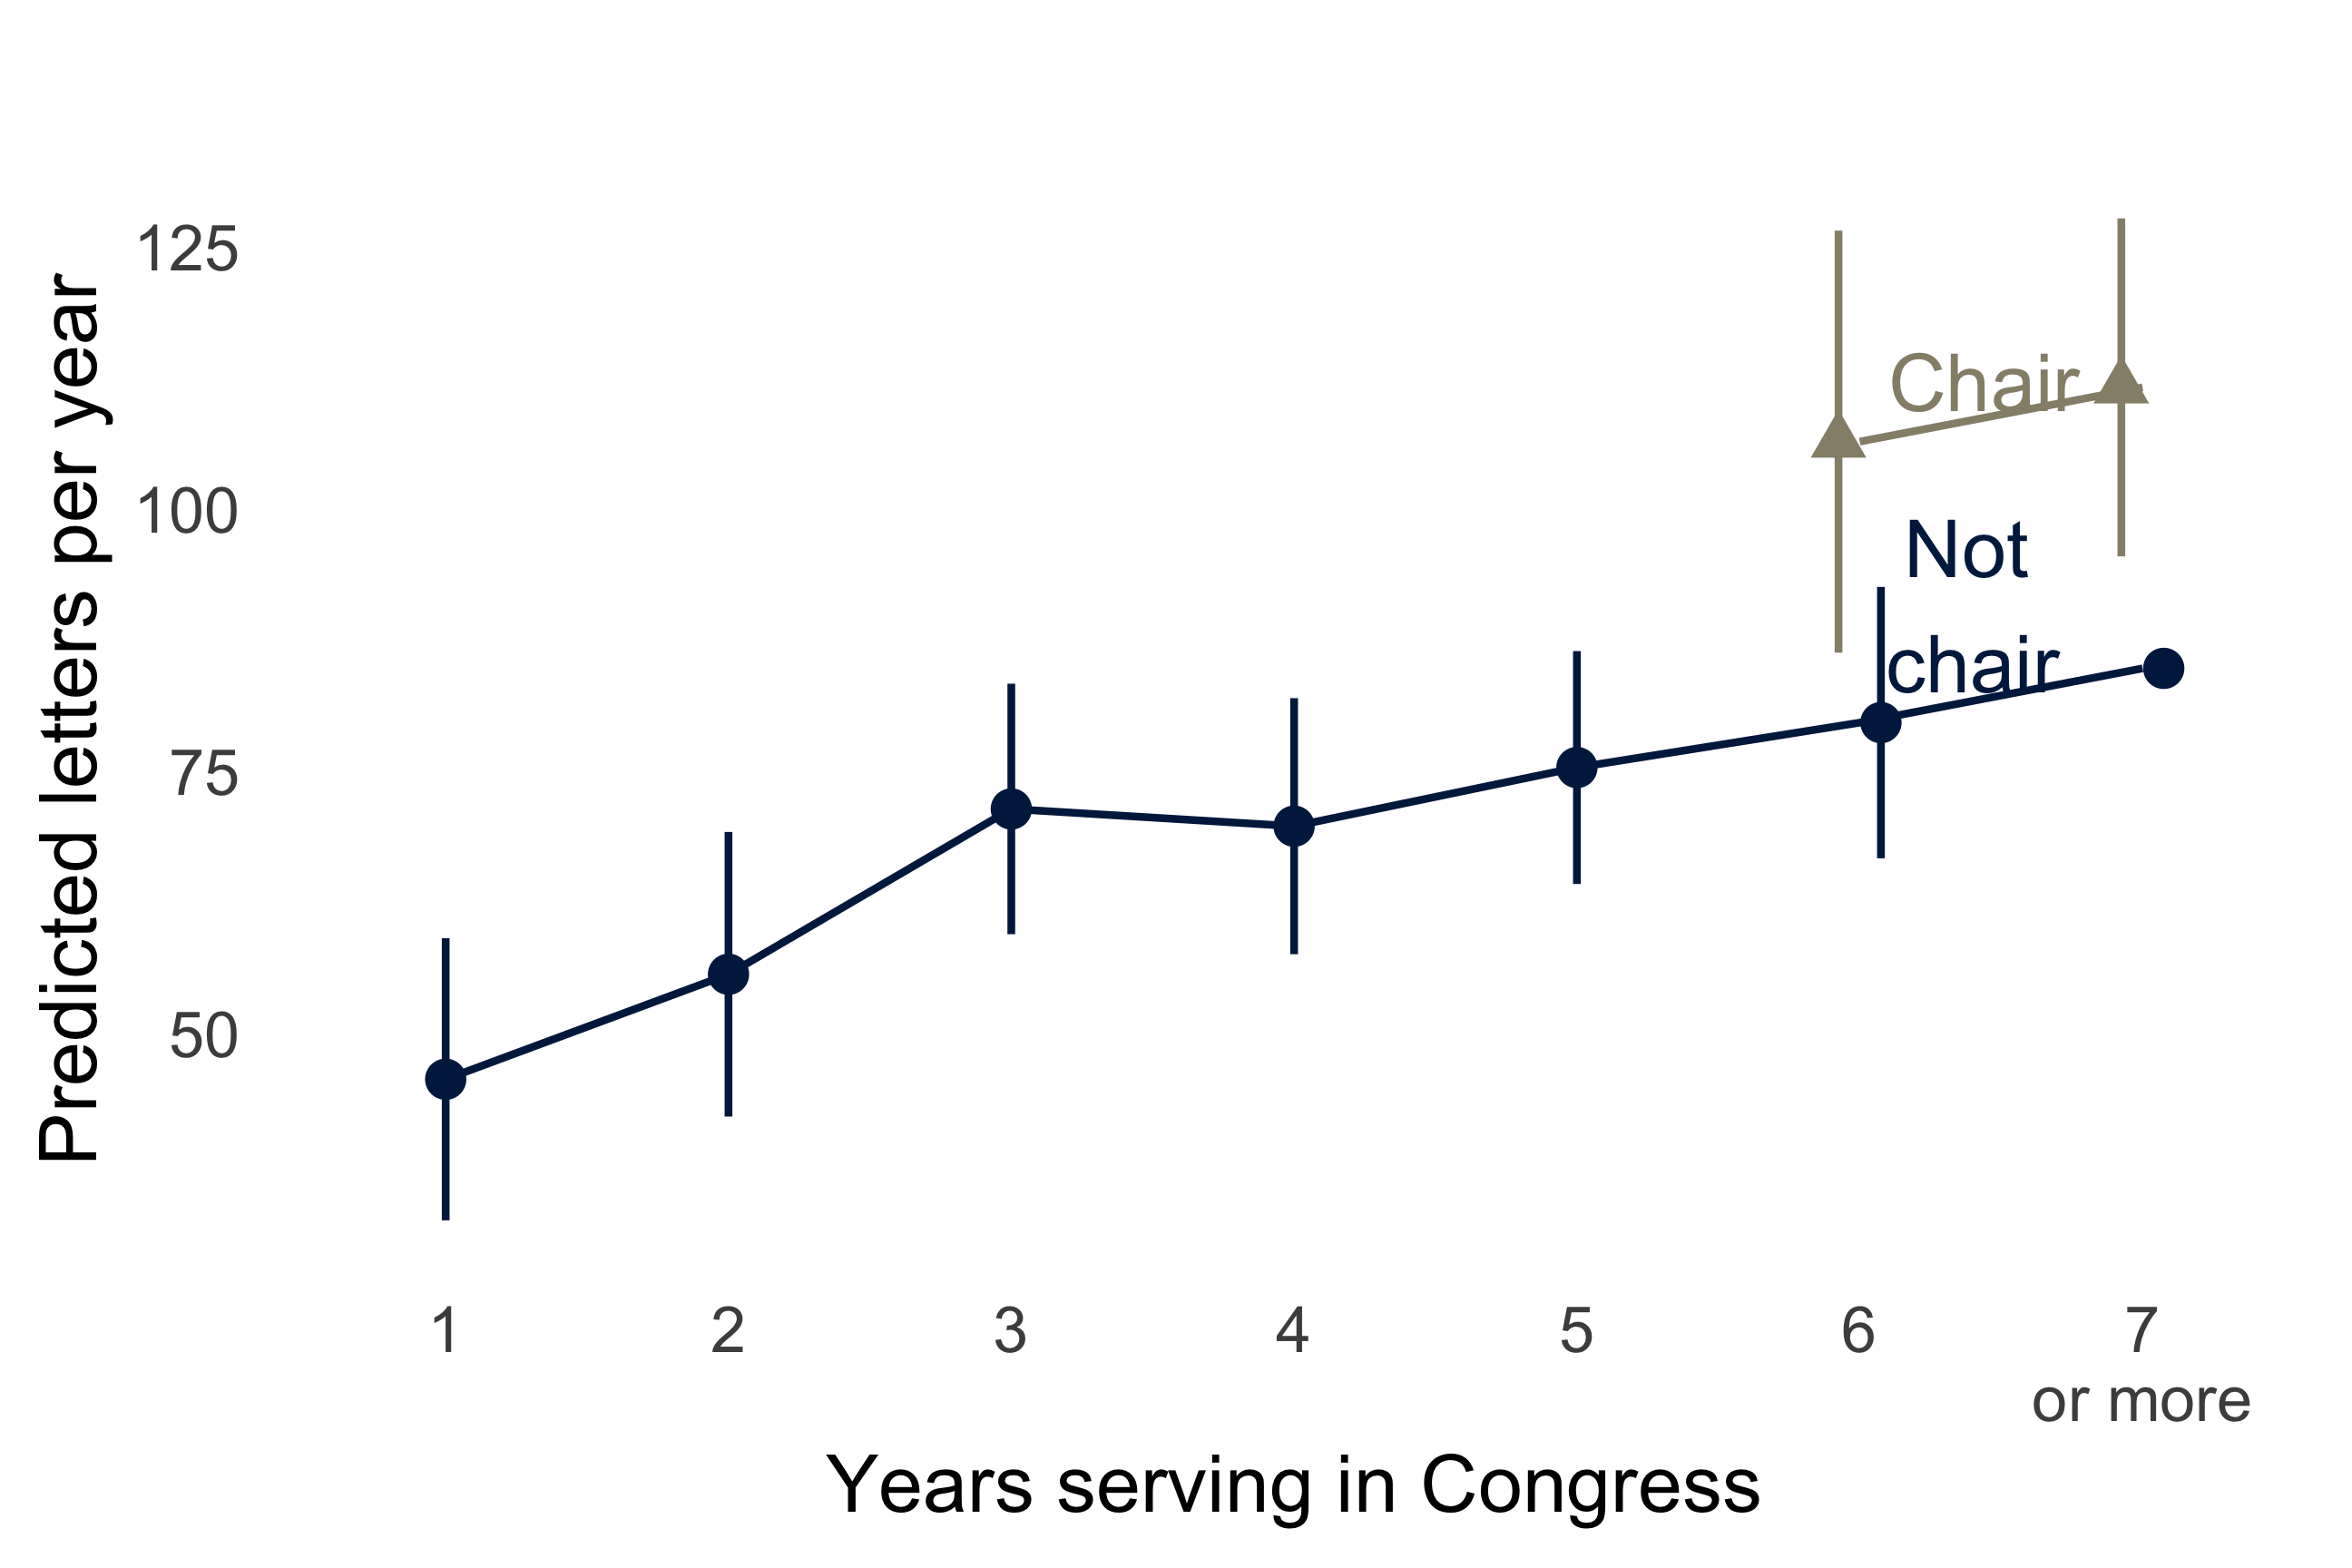
\includegraphics[width = .8\textwidth]{figs/m-total-predicted-4}
\end{figure}

Figure \ref{f:m-total-predicted-time} shows the predicted total number of letters in Congress and committee chair status (comparing predictions for counterfactuals where the same legislator did and did not receive a chairmanship in their sixth year).\footnote{Predictions are based on a legislator-agency pair where (1) the legislators' average annual contacts equaled the overall average, (2) the legislators' number of contacts with the agency equal the average received by that agency, (3) and the agency received an average number of letters.} 


Figure \ref{f:m-total-predicted-time} uses the coefficients in legislators' first six years in office from Table \ref{t:models_total}. The reference group is representatives who have served longer than six years.\footnote{Interpreting these coefficients requires that we assume the effects of tenure and committee assignment are linearly separable. This assumption is reasonable because most legislators do not become chairs, ranking members, or join prestige committees in their first six years, and almost none in their first two years.} 

The first column of Table \ref{t:models_total} shows large cross-sectional differences: legislators in their first year make fewer contacts than more experienced legislators. First-year legislators make approximately 0.255 fewer requests per agency than legislators in their seventh year or beyond. This difference shrinks in the second year and then is mostly gone. But we advise caution in interpreting the differences in Column 1 because they conflate the effect of increased experience with other characteristics that may correlate with whether a legislator remains in office and, thus whether we observe them in later years.   

To account for possible differences in legislators who obtain different levels of tenure, the second column of Table \ref{t:models_total} estimates the difference-in-differences specification in Equation \ref{e:diff1}. The tenure coefficients show that legislators provide less constituency service in their first year in office. As they acquire experience, they make more requests to federal agencies. In their first year in office, legislators provide 21.33 (90 $\times$ (.512 - .275)) fewer requests per agency than legislators in their second year and 29.07 (90 $\times$ (.512 - .189)) fewer requests than legislators in their third year---both differences are statistically significant at conventional levels. The overall increase in levels of constituency service from a legislator's first to third year is similar in size to the increase that comes from becoming a member of the oversight committee. Once legislators enter their fourth year, their behavior no longer differs from more experienced legislators. We find small and statistically insignificant differences for legislators in their fourth through sixth years. As legislators acquire experience and build their office's organizational capacity in their first two years, they make more contacts with federal agencies.  

As with the analysis of committee prestige, the findings in Table \ref{t:models_total} are robust to alternative specifications. Despite the difference-in-difference design, we might still be concerned that the set of legislators who served a third year differs from those who served a first year. If this were the case, our findings would result from both the experience and a selection effect due to House members who win reelection, a potential indication that they are better able to perform the job than other legislators. To address the potentially different samples each year, the third column of Table \ref{t:models_total} assesses the changes in the number of contacts of federal agencies for legislators who serve for at least three years. The pattern is similar: legislators initially provide less constituency service in their first two years than in subsequent years. Column 4 in Table \ref{t:models_total} shows that the results are robust to analyzing $\log(Y_{ijt} + 1)$, ensuring that our results are not because of outliers. Additional models below estimate the same models as Table \ref{t:models_total} on hand-coded subsets of the data, showing similar results. 


 




\subsection{Constituency Service Only}

\begin{table}[hbt!]
\caption{The Effect Experience and Institutional Power on Constituency Service} \label{t:models_con}
\begin{minipage}{\textwidth}
\begin{center}
\begin{tabular}[t]{lcccc}
\toprule
  & (1) & (2) & (3) & (4)\\
\midrule
\textbf{Dependent Variable} & \textbf{Count} & \textbf{Count} & \textbf{Count} & \textbf{Log(Count+1)}\\
\midrule
Committee Chair & \num{0.302} & \num{0.040} & \num{0.044} & \num{0.012}\\
 & (\num{0.108}) & (\num{0.064}) & (\num{0.064}) & (\num{0.007})\\
Ranking Member & \num{0.503} & \num{0.054} & \num{0.070} & \num{0.012}\\
 & (\num{0.108}) & (\num{0.067}) & (\num{0.067}) & (\num{0.007})\\
Prestige Committee & \num{0.321} & \num{0.031} & \num{0.025} & \num{0.013}\\
 & (\num{0.049}) & (\num{0.036}) & (\num{0.036}) & (\num{0.007})\\
First Year & \num{-0.138} & \num{-0.276} & \num{-0.265} & \num{-0.059}\\
 & (\num{0.040}) & (\num{0.055}) & (\num{0.054}) & (\num{0.008})\\
Second Year & \num{0.009} & \num{-0.128} & \num{-0.142} & \num{-0.019}\\
 & (\num{0.046}) & (\num{0.053}) & (\num{0.052}) & (\num{0.008})\\
Third Year & \num{0.030} & \num{-0.070} & \num{-0.088} & \num{-0.011}\\
 & (\num{0.047}) & (\num{0.047}) & (\num{0.046}) & (\num{0.007})\\
Fourth Year & \num{0.061} & \num{-0.055} & \num{-0.072} & \num{-0.006}\\
 & (\num{0.052}) & (\num{0.046}) & (\num{0.045}) & (\num{0.006})\\
Fifth Year & \num{0.001} & \num{-0.069} & \num{-0.064} & \num{-0.011}\\
 & (\num{0.044}) & (\num{0.034}) & (\num{0.033}) & (\num{0.005})\\
Sixth Year & \num{0.070} & \num{0.008} & \num{0.018} & \num{-0.004}\\
 & (\num{0.056}) & (\num{0.044}) & (\num{0.043}) & (\num{0.005})\\
\midrule
Majority & \checkmark & \checkmark & \checkmark & \checkmark\\
Presidents` Party & \checkmark & \checkmark & \checkmark & \checkmark\\
All Legislators & \checkmark & \checkmark &  & \checkmark\\
Served At Least 2nd Term &  &  & \checkmark & \\
Observations & \num{412111} & \num{412111} & \num{388997} & \num{412111}\\
Year x Agency FE & \checkmark & \checkmark & \checkmark & \checkmark\\
Legislator x Agency FE &  & \checkmark & \checkmark & \checkmark\\
\bottomrule
\multicolumn{5}{l}{\rule{0pt}{1em}\footnotesize Robust standard errors in parentheses, clustered by legislator.}\\
\end{tabular}
 % this one is from replication.rmd
\end{center}
\footnotetext{This table shows how the number of contacts hand-coded as constituecy service changes as legislators acquire more expiernece and power in Congress. Column 1 shows the average differences across committee assignments and years in Congress. Column 2 presents the difference-in-differences estimates. Column 3 subsets to legislators who serve at least 3 years in Congress. Column 4 takes the Log of the counts + 1 as the dependent variable.}
\end{minipage}
\end{table}

Table \ref{t:models_con} is identical to Table \ref{t:models_total} except that we subset the data to only legislator requests hand-coded as constituency service. 
Model 2 (Column 2 of Table \ref{t:models_con} and Figure \ref{f:m-con-predicted}) provide the estimated effects from the difference-in-differences specification in Equation \ref{e:diff1}. More experience increases the level of constituency service that legislators provide. The effect of being a committee chair is positive but not significant at the .05 level. We estimate that the experience gained between the first and second year in Congress causes an increase of 0.15 requests \textit{per agency}. The experience gained between the first and seventh years causes an increase of 0.28 per agency. Across all 90 agencies, this represents an increase of approximately 25 additional requests per year, 38.6\% of the average number of requests per year in our data. There is a smaller increase after the second year. The experience gained between the second and seventh year causes an increase of 0.13 per agency, an increase of approximately 12 additional requests per year, 38.6\% of the average number of requests per year in our data.


\begin{figure}[hbt!]
\centering
\caption{Predicted Number of Constituency Service Requests} \label{f:m-con-predicted}
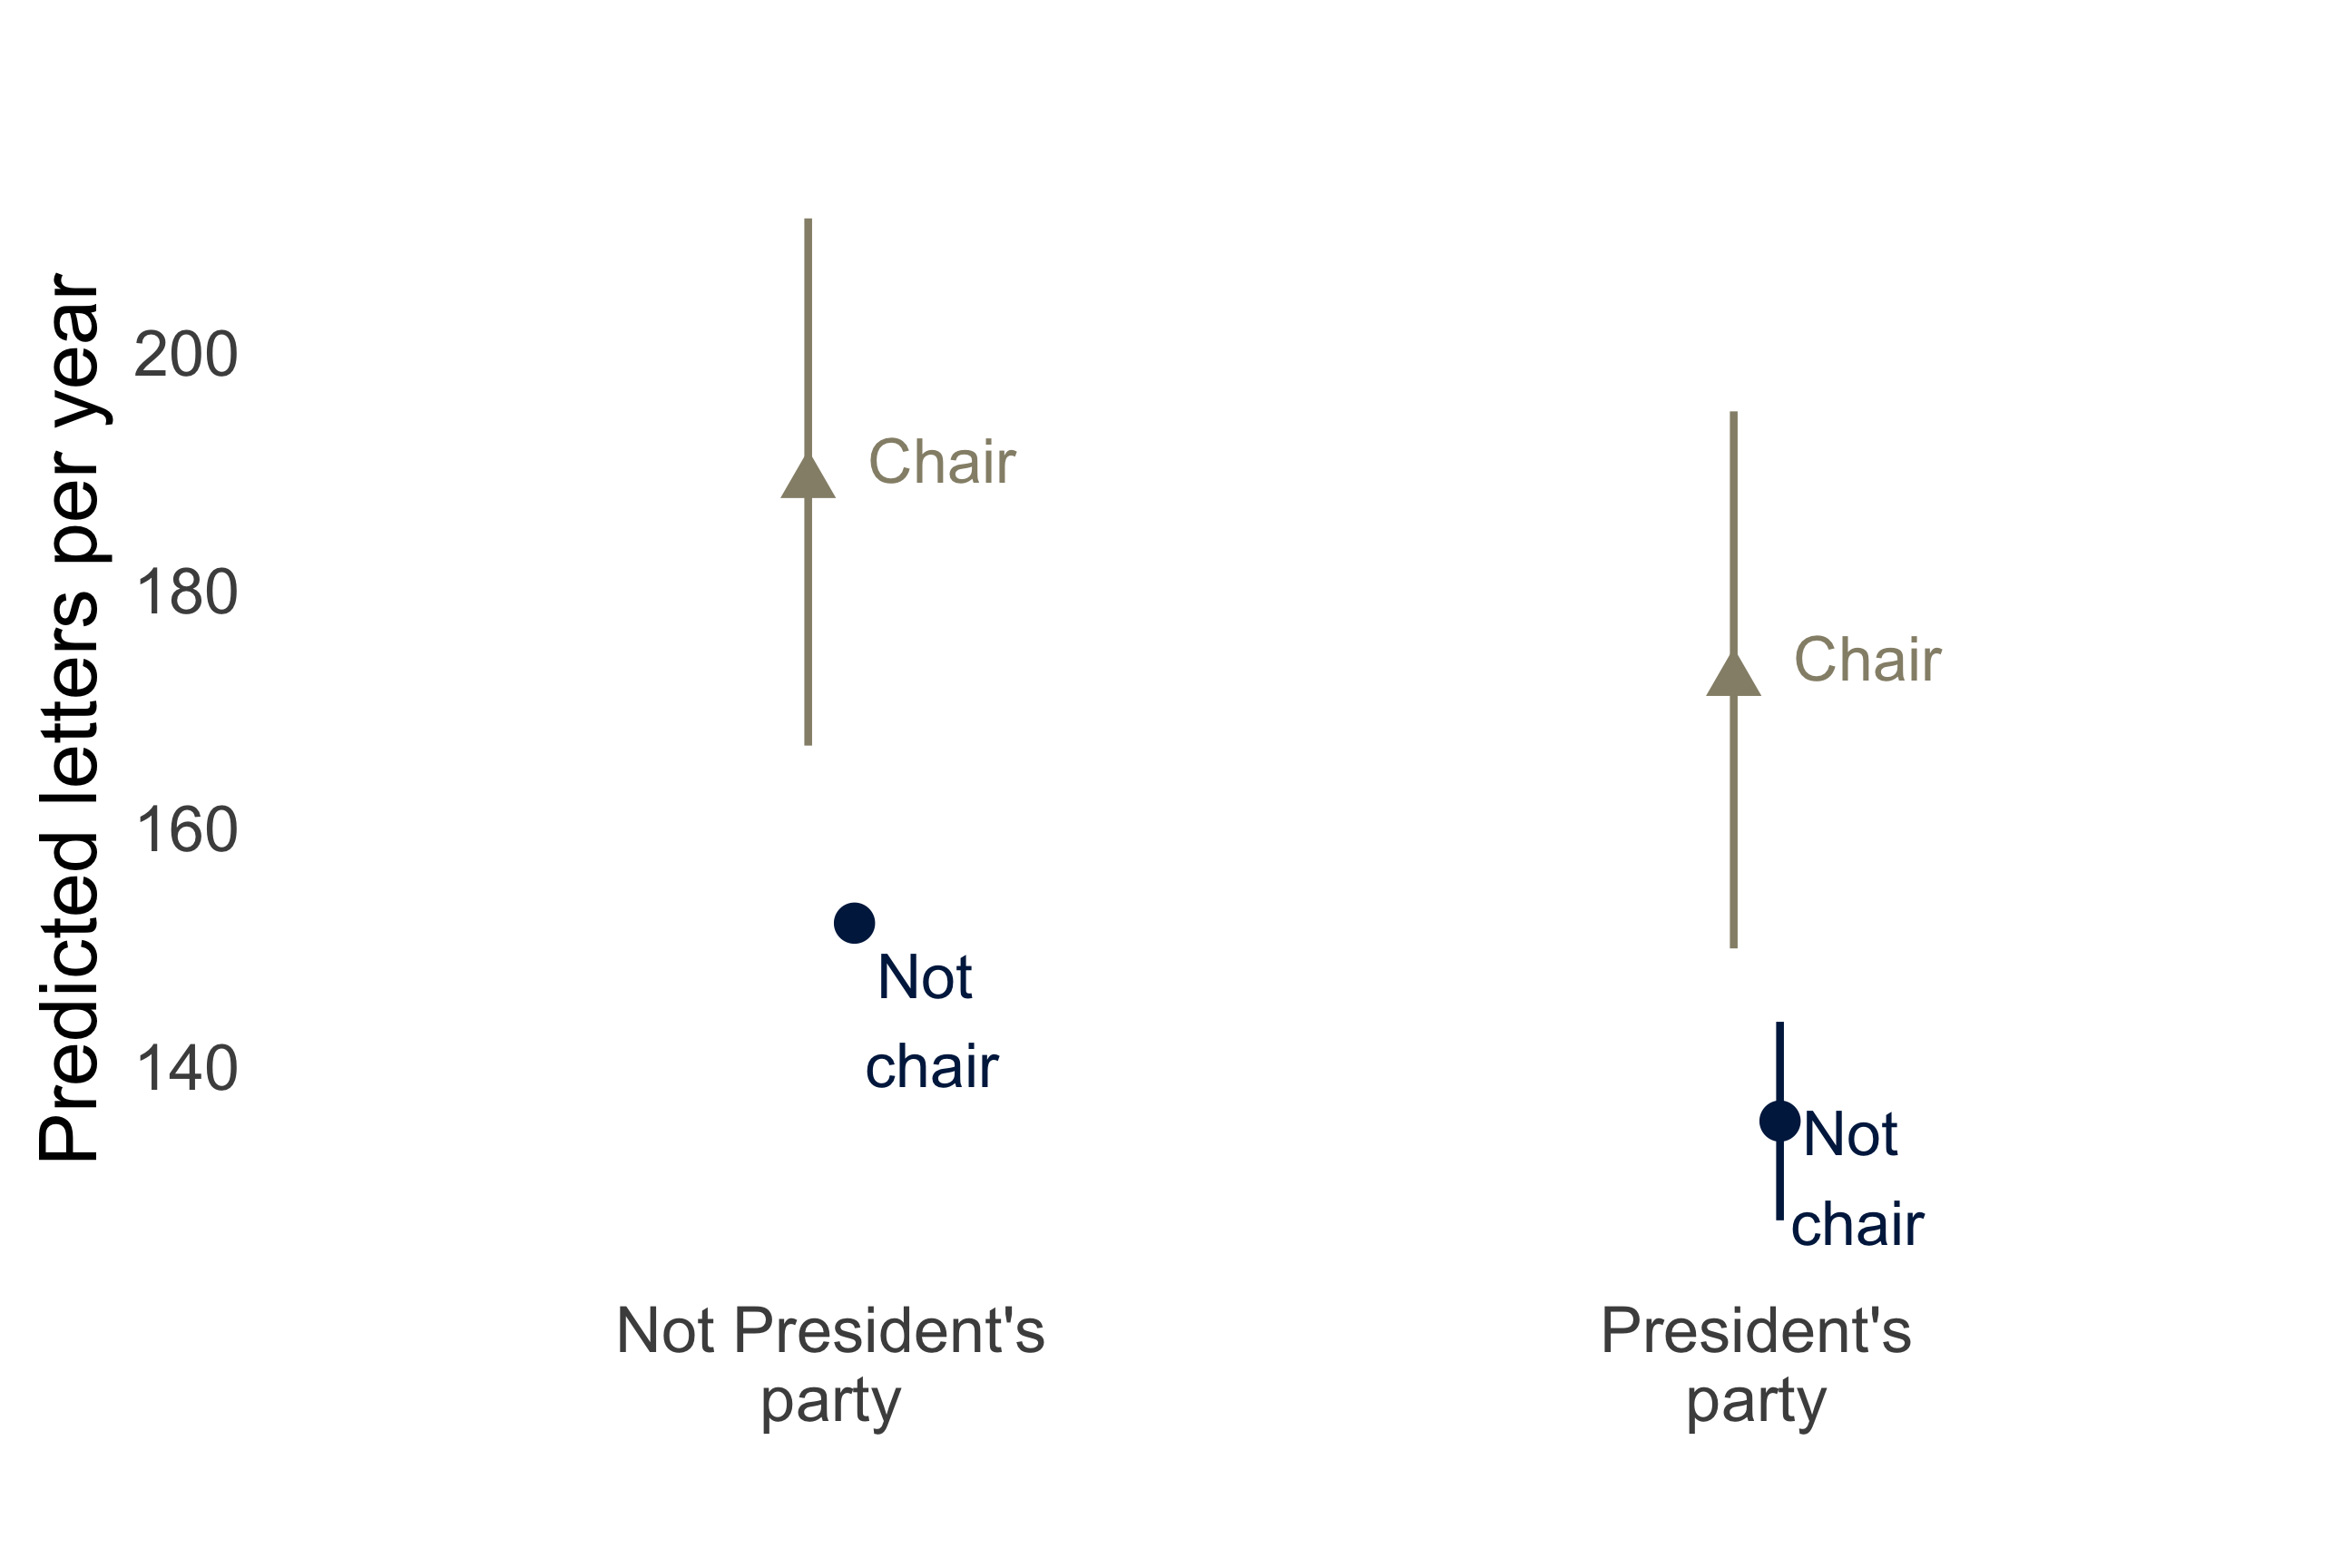
\includegraphics[width = .49\textwidth]{figs/m-con-predicted-1}
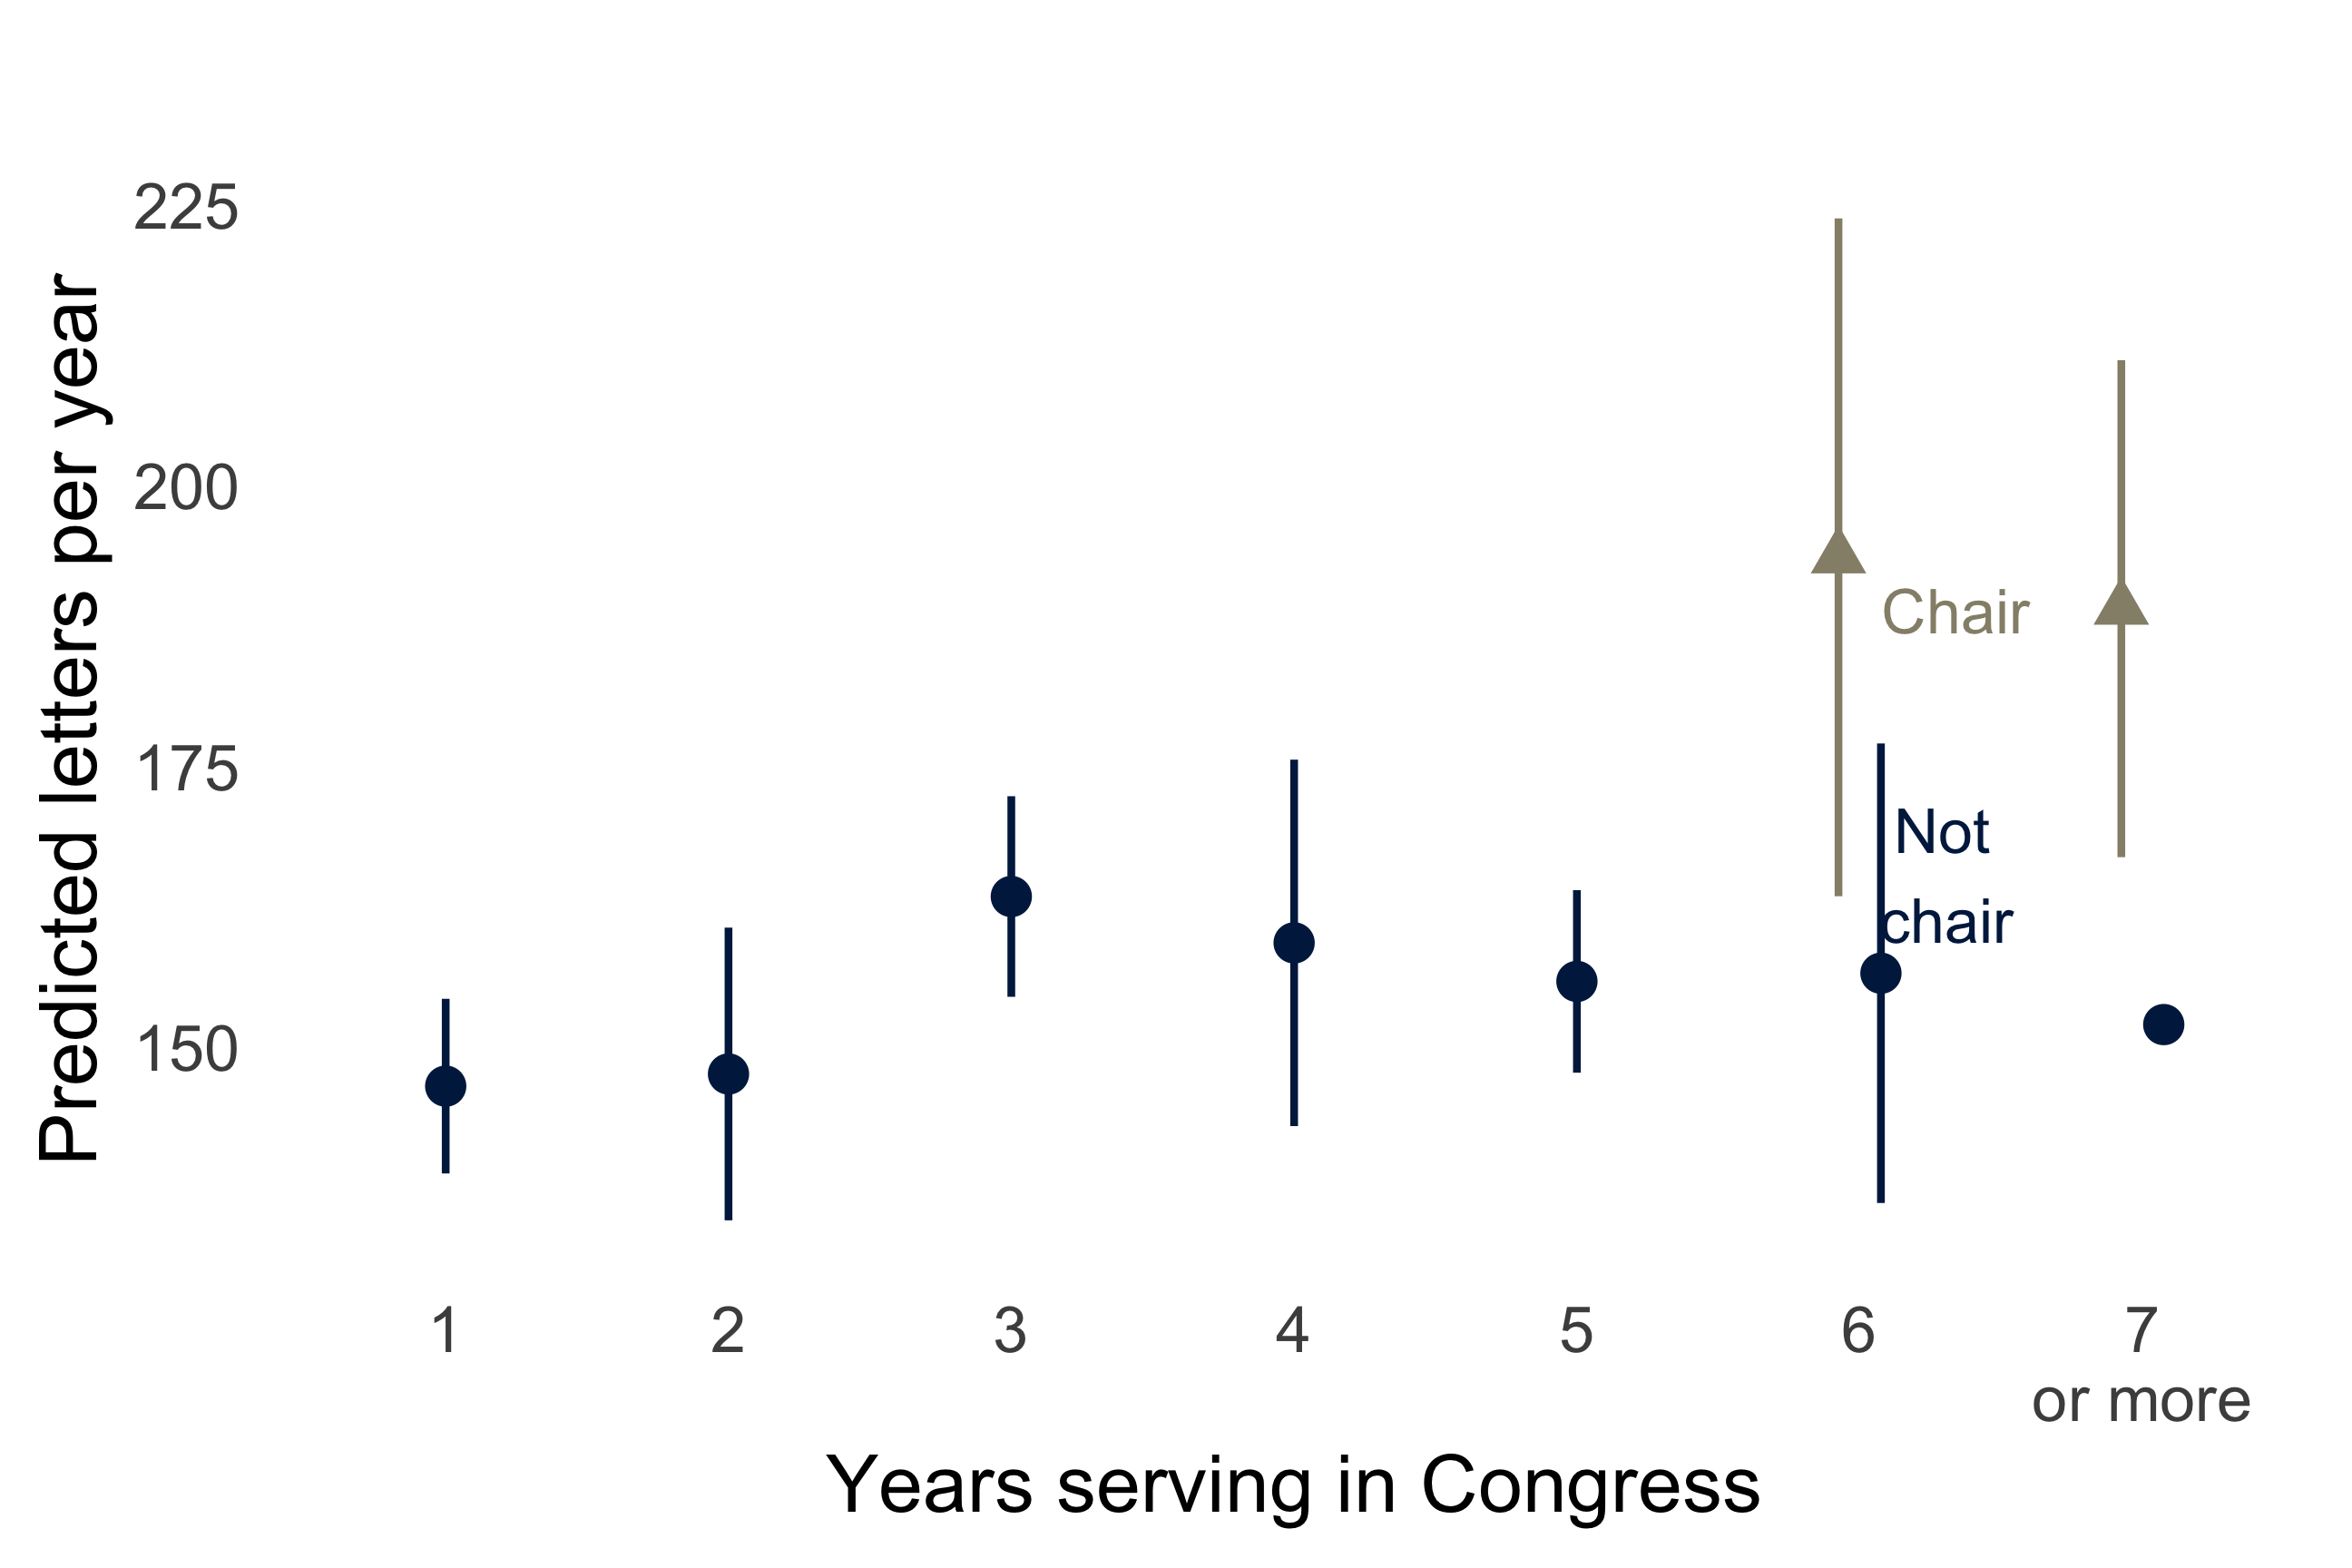
\includegraphics[width = .49\textwidth]{figs/m-con-predicted-2}
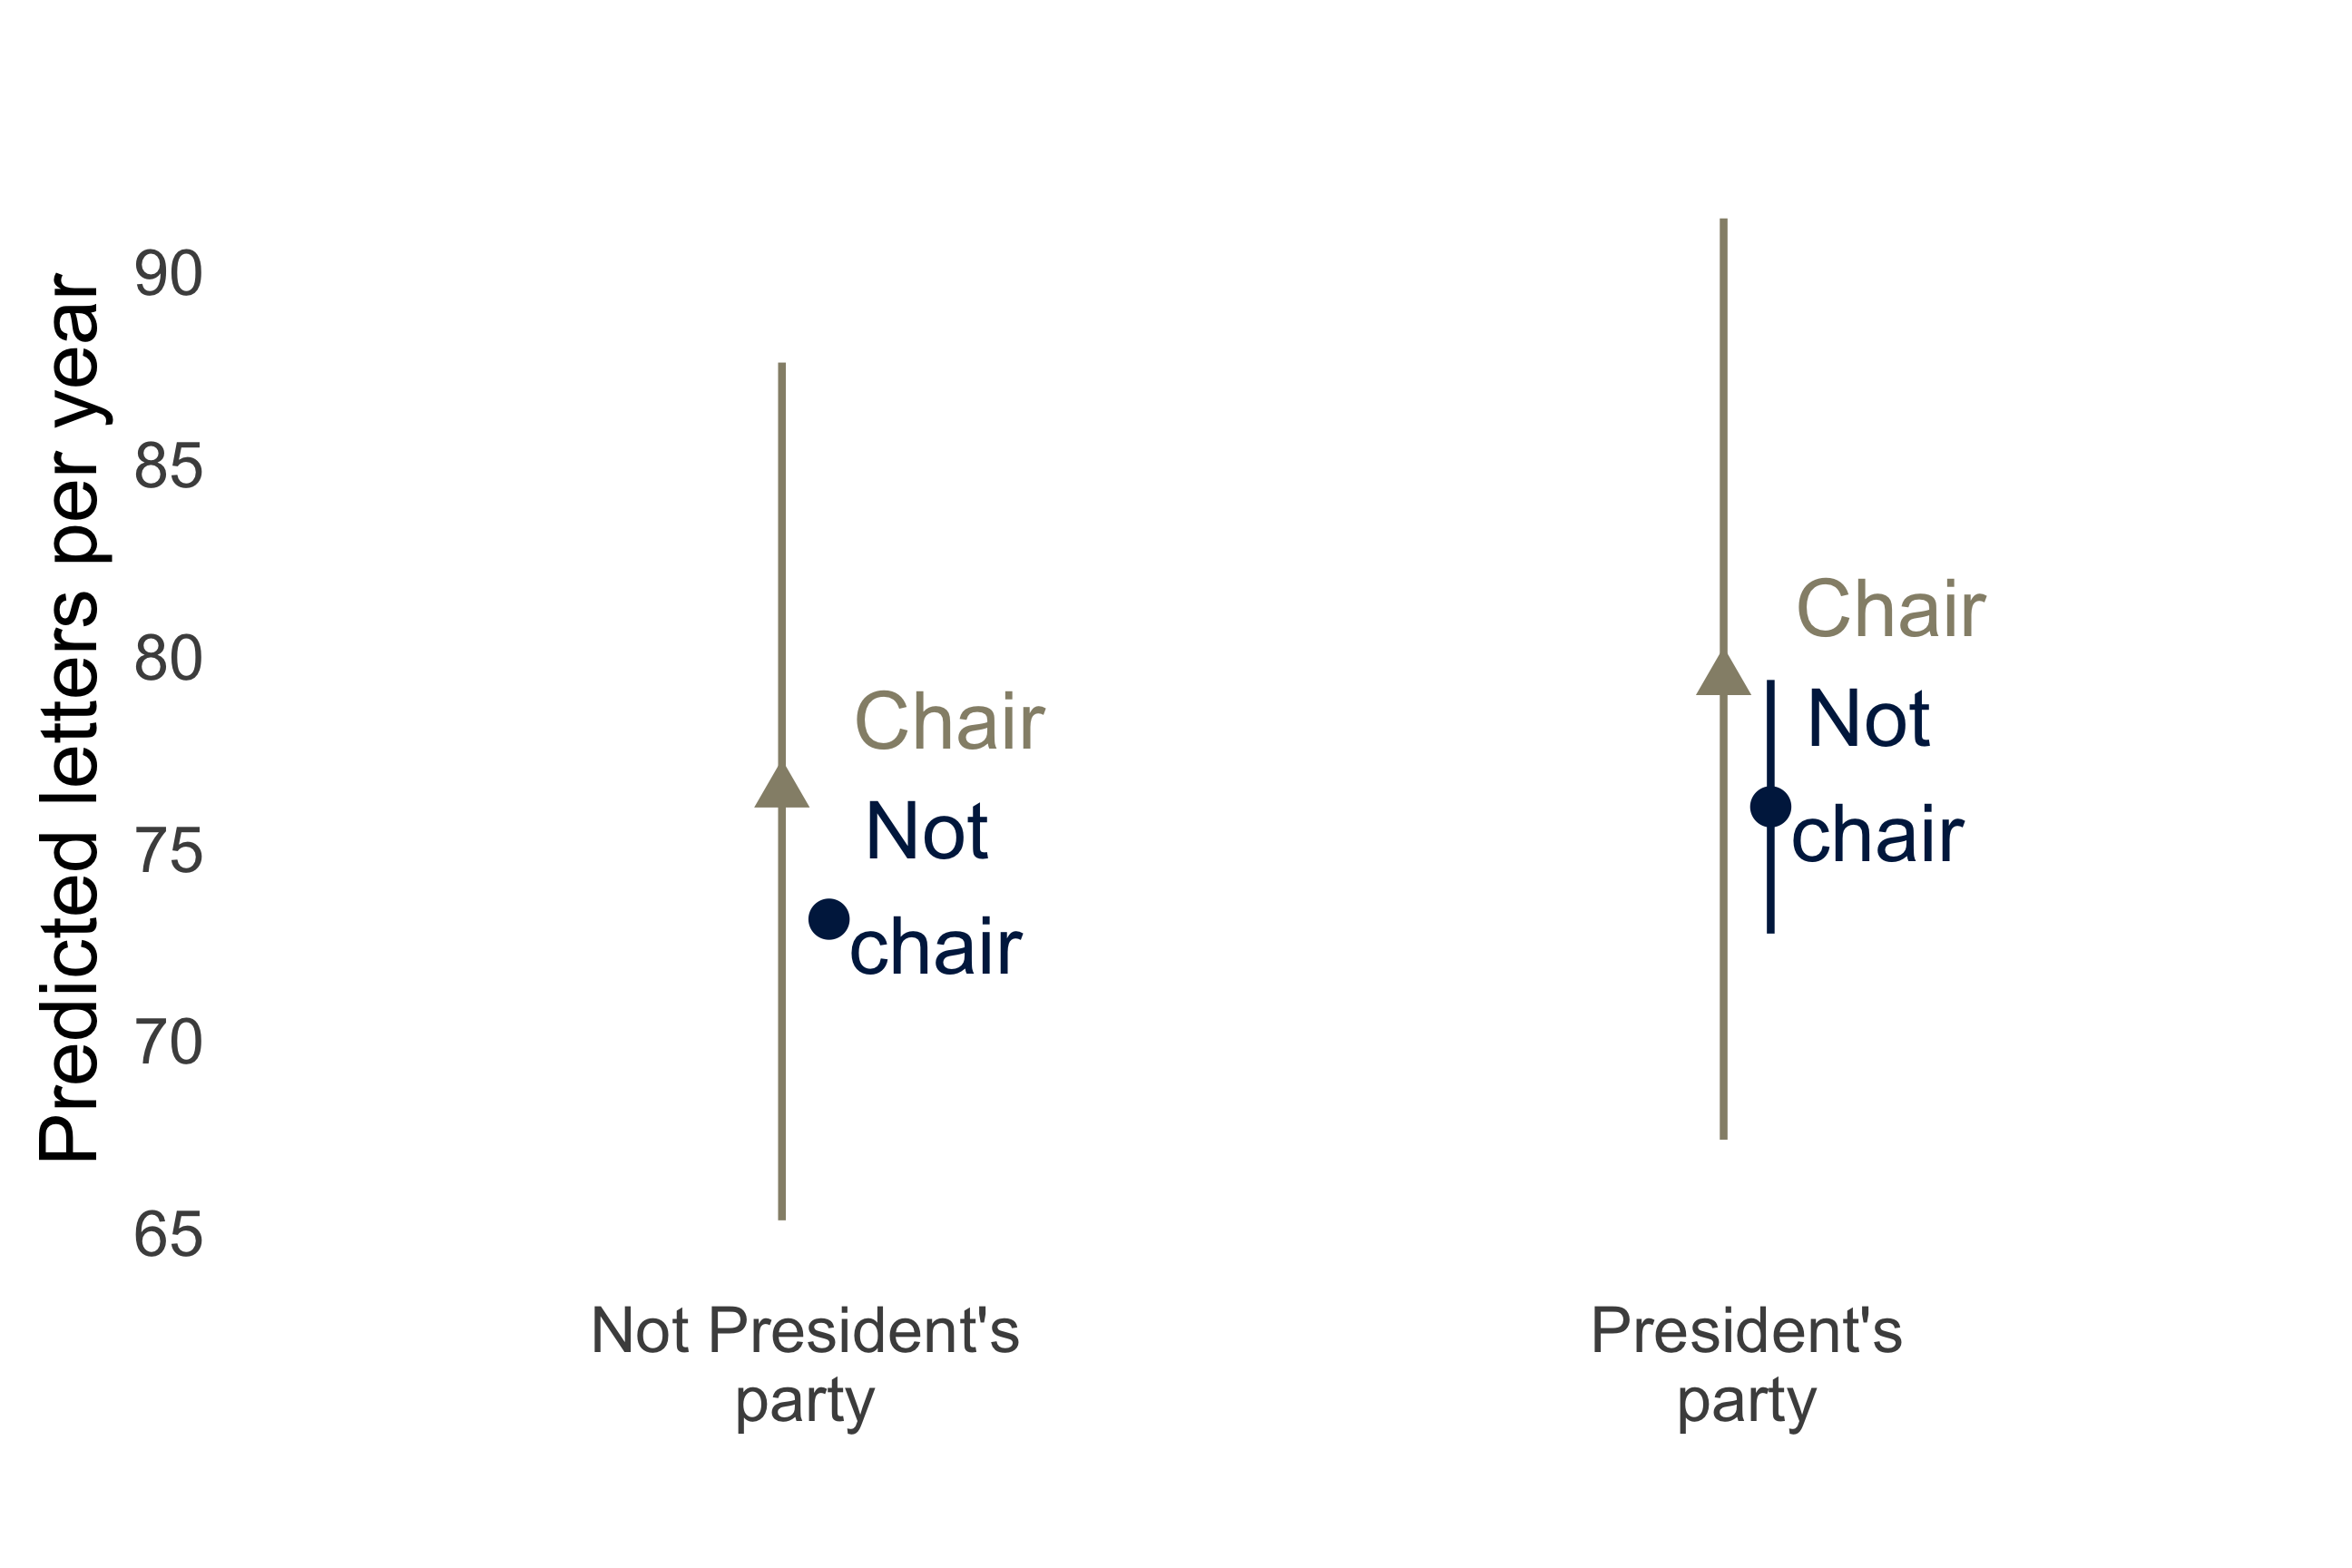
\includegraphics[width = .49\textwidth]{figs/m-con-predicted-3}
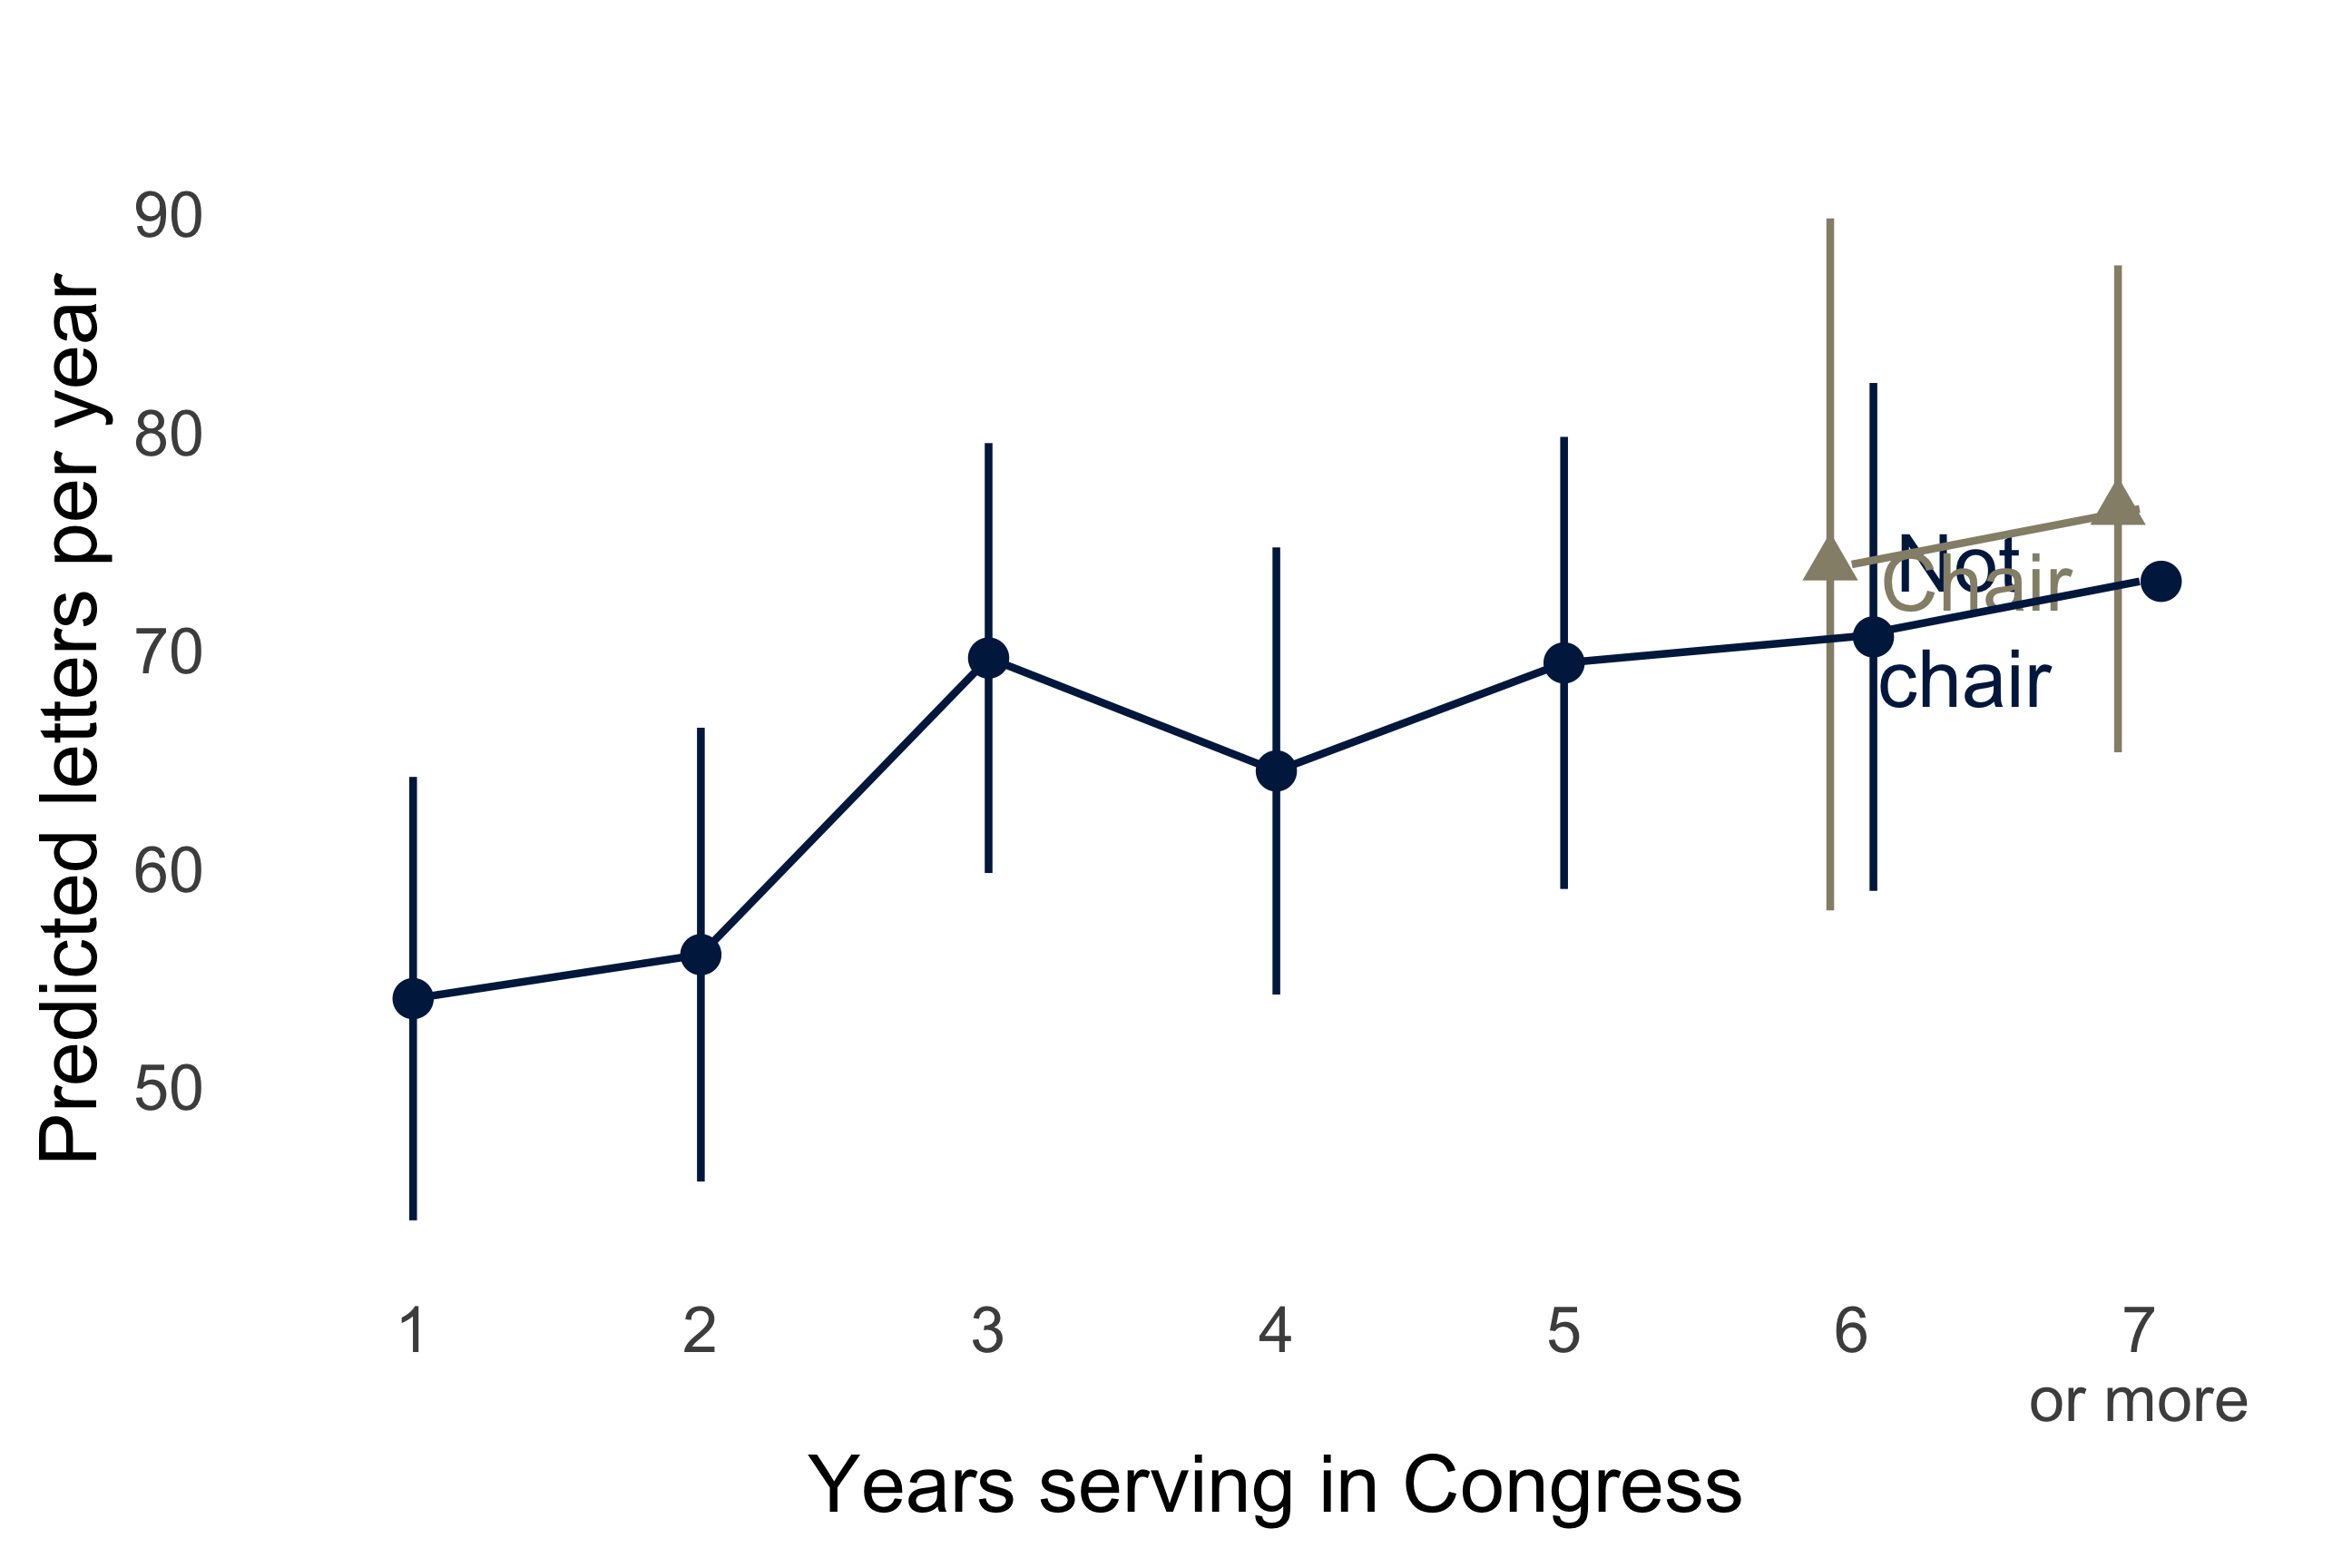
\includegraphics[width = .49\textwidth]{figs/m-con-predicted-4}

\end{figure}

\subsection{Policy Work Only}

\begin{table}[hbt!]
\caption{The Effect Experience and Institutional Power on Policy Work} \label{t:models_policy}
\begin{minipage}{\textwidth}
\begin{center}
\begin{tabular}[t]{lcccc}
\toprule
  & (1) & (2) & (3) & (4)\\
\midrule
\textbf{Dependent Variable} & \textbf{Count} & \textbf{Count} & \textbf{Count} & \textbf{Log(Count+1)}\\
\midrule
Committee Chair & \num{0.199} & \num{0.158} & \num{0.159} & \num{0.036}\\
 & (\num{0.027}) & (\num{0.034}) & (\num{0.034}) & (\num{0.007})\\
Ranking Member & \num{0.145} & \num{0.090} & \num{0.092} & \num{0.025}\\
 & (\num{0.028}) & (\num{0.024}) & (\num{0.024}) & (\num{0.005})\\
Prestige Committee & \num{0.049} & \num{0.031} & \num{0.031} & \num{0.010}\\
 & (\num{0.009}) & (\num{0.010}) & (\num{0.010}) & (\num{0.003})\\
First Year & \num{-0.076} & \num{-0.076} & \num{-0.070} & \num{-0.030}\\
 & (\num{0.007}) & (\num{0.016}) & (\num{0.016}) & \vphantom{1} (\num{0.004})\\
Second Year & \num{-0.045} & \num{-0.042} & \num{-0.040} & \num{-0.018}\\
 & (\num{0.007}) & (\num{0.016}) & (\num{0.016}) & (\num{0.004})\\
Third Year & \num{-0.042} & \num{-0.031} & \num{-0.033} & \num{-0.013}\\
 & (\num{0.008}) & (\num{0.013}) & (\num{0.013}) & (\num{0.004})\\
Fourth Year & \num{-0.021} & \num{-0.011} & \num{-0.013} & \num{-0.006}\\
 & (\num{0.009}) & (\num{0.013}) & (\num{0.013}) & (\num{0.004})\\
Fifth Year & \num{-0.022} & \num{-0.009} & \num{-0.011} & \num{-0.006}\\
 & (\num{0.009}) & (\num{0.011}) & (\num{0.011}) & (\num{0.003})\\
Sixth Year & \num{-0.011} & \num{0.002} & \num{0.003} & \num{-0.006}\\
 & (\num{0.012}) & (\num{0.012}) & (\num{0.012}) & (\num{0.003})\\
\midrule
Majority & \checkmark & \checkmark & \checkmark & \checkmark\\
President's Party & \checkmark & \checkmark & \checkmark & \checkmark\\
All Legislators & \checkmark & \checkmark &  & \checkmark\\
Served At Least 2nd Term &  &  & \checkmark & \\
Observations & \num{412111} & \num{412111} & \num{388997} & \num{412111}\\
Year x Agency FE & \checkmark & \checkmark & \checkmark & \checkmark\\
Legislator x Agency FE &  & \checkmark & \checkmark & \checkmark\\
\bottomrule
\multicolumn{5}{l}{\rule{0pt}{1em}\footnotesize Robust standard errors in parentheses, clustered by legislator.}\\
\end{tabular}
 % this one is from replication.rmd
\end{center}
\footnotetext{This table shows how the number of hand-coded policy work contacts changes as legislators acquire more experience and power in Congress. Column 1 shows the average differences across committee assignments and years in Congress. Column 2 presents the difference-in-differences estimates. Column 3 subsets to legislators who serve at least 3 years in Congress. Column 4 takes the Log of the counts + 1 as the dependent variable.}
\end{minipage}
\end{table}


Table \ref{t:models_policy} is identical to Table \ref{t:models_total} except that we subset the data to only legislator requests hand-coded as policy work. 
Column 2 of Table \ref{t:models_policy} and Figure \ref{f:m-policy-predicted}) provide the estimated effects from the difference-in-differences specification in Equation \ref{e:diff1}. Across all measures of institutional power, we find that more power increases the level of policy work that legislators provide. Consider first the effect of being a committee chair. We estimate that becoming a committee chair causes an increase of 0.16 policy requests \textit{per agency} (95-percent confidence interval [0.09, 0.22]). Across all 90 agencies, this represents an increase of approximately 14 additional requests per year, 92.6\% of the average number of requests per year in our data. There is a smaller increase for individuals who become ranking members and those who join a Prestige Committee, though the increase is statistically significant for the prestige committee. Becoming a ranking member of a committee causes an increase of 0.09 contacts per agency, while joining a prestige committee causes a 0.16 per agency increase in the number of contacts a member of Congress makes.

\begin{figure}[hbt!]
\centering
\caption{Predicted Number of Policy Requests} \label{f:m-policy-predicted}
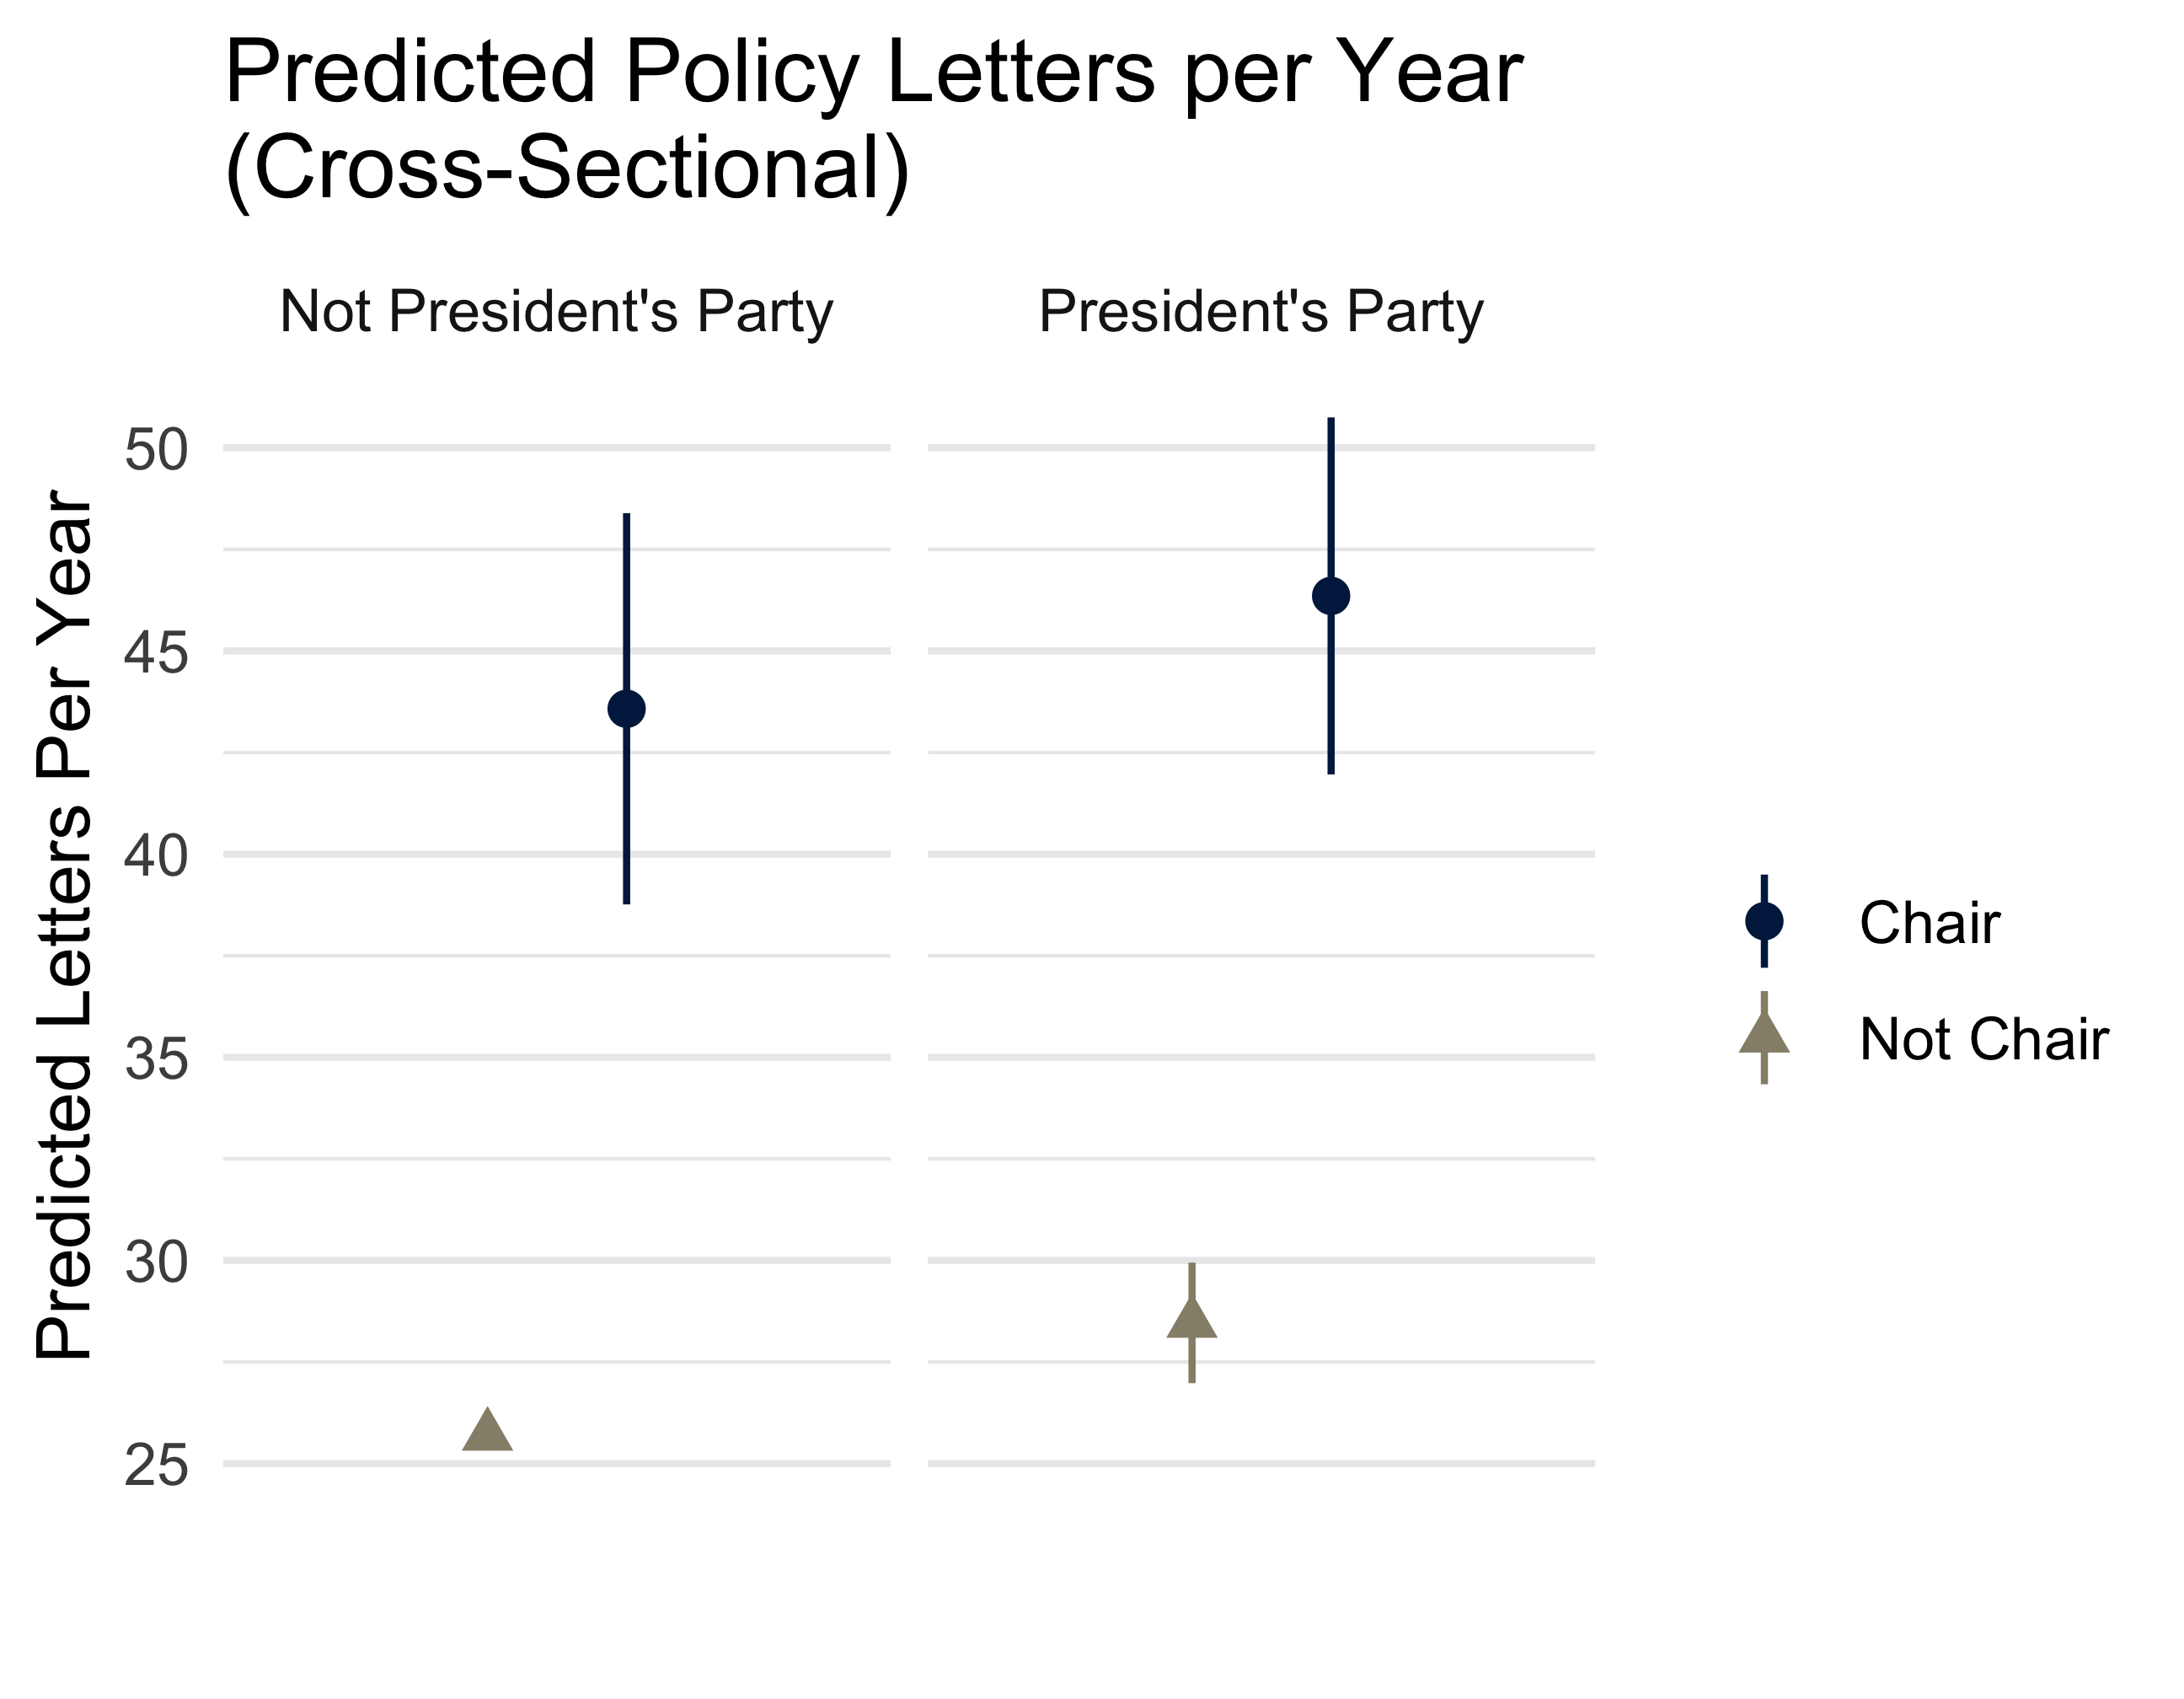
\includegraphics[width = .48\textwidth]{figs/m-policy-predicted-1} 
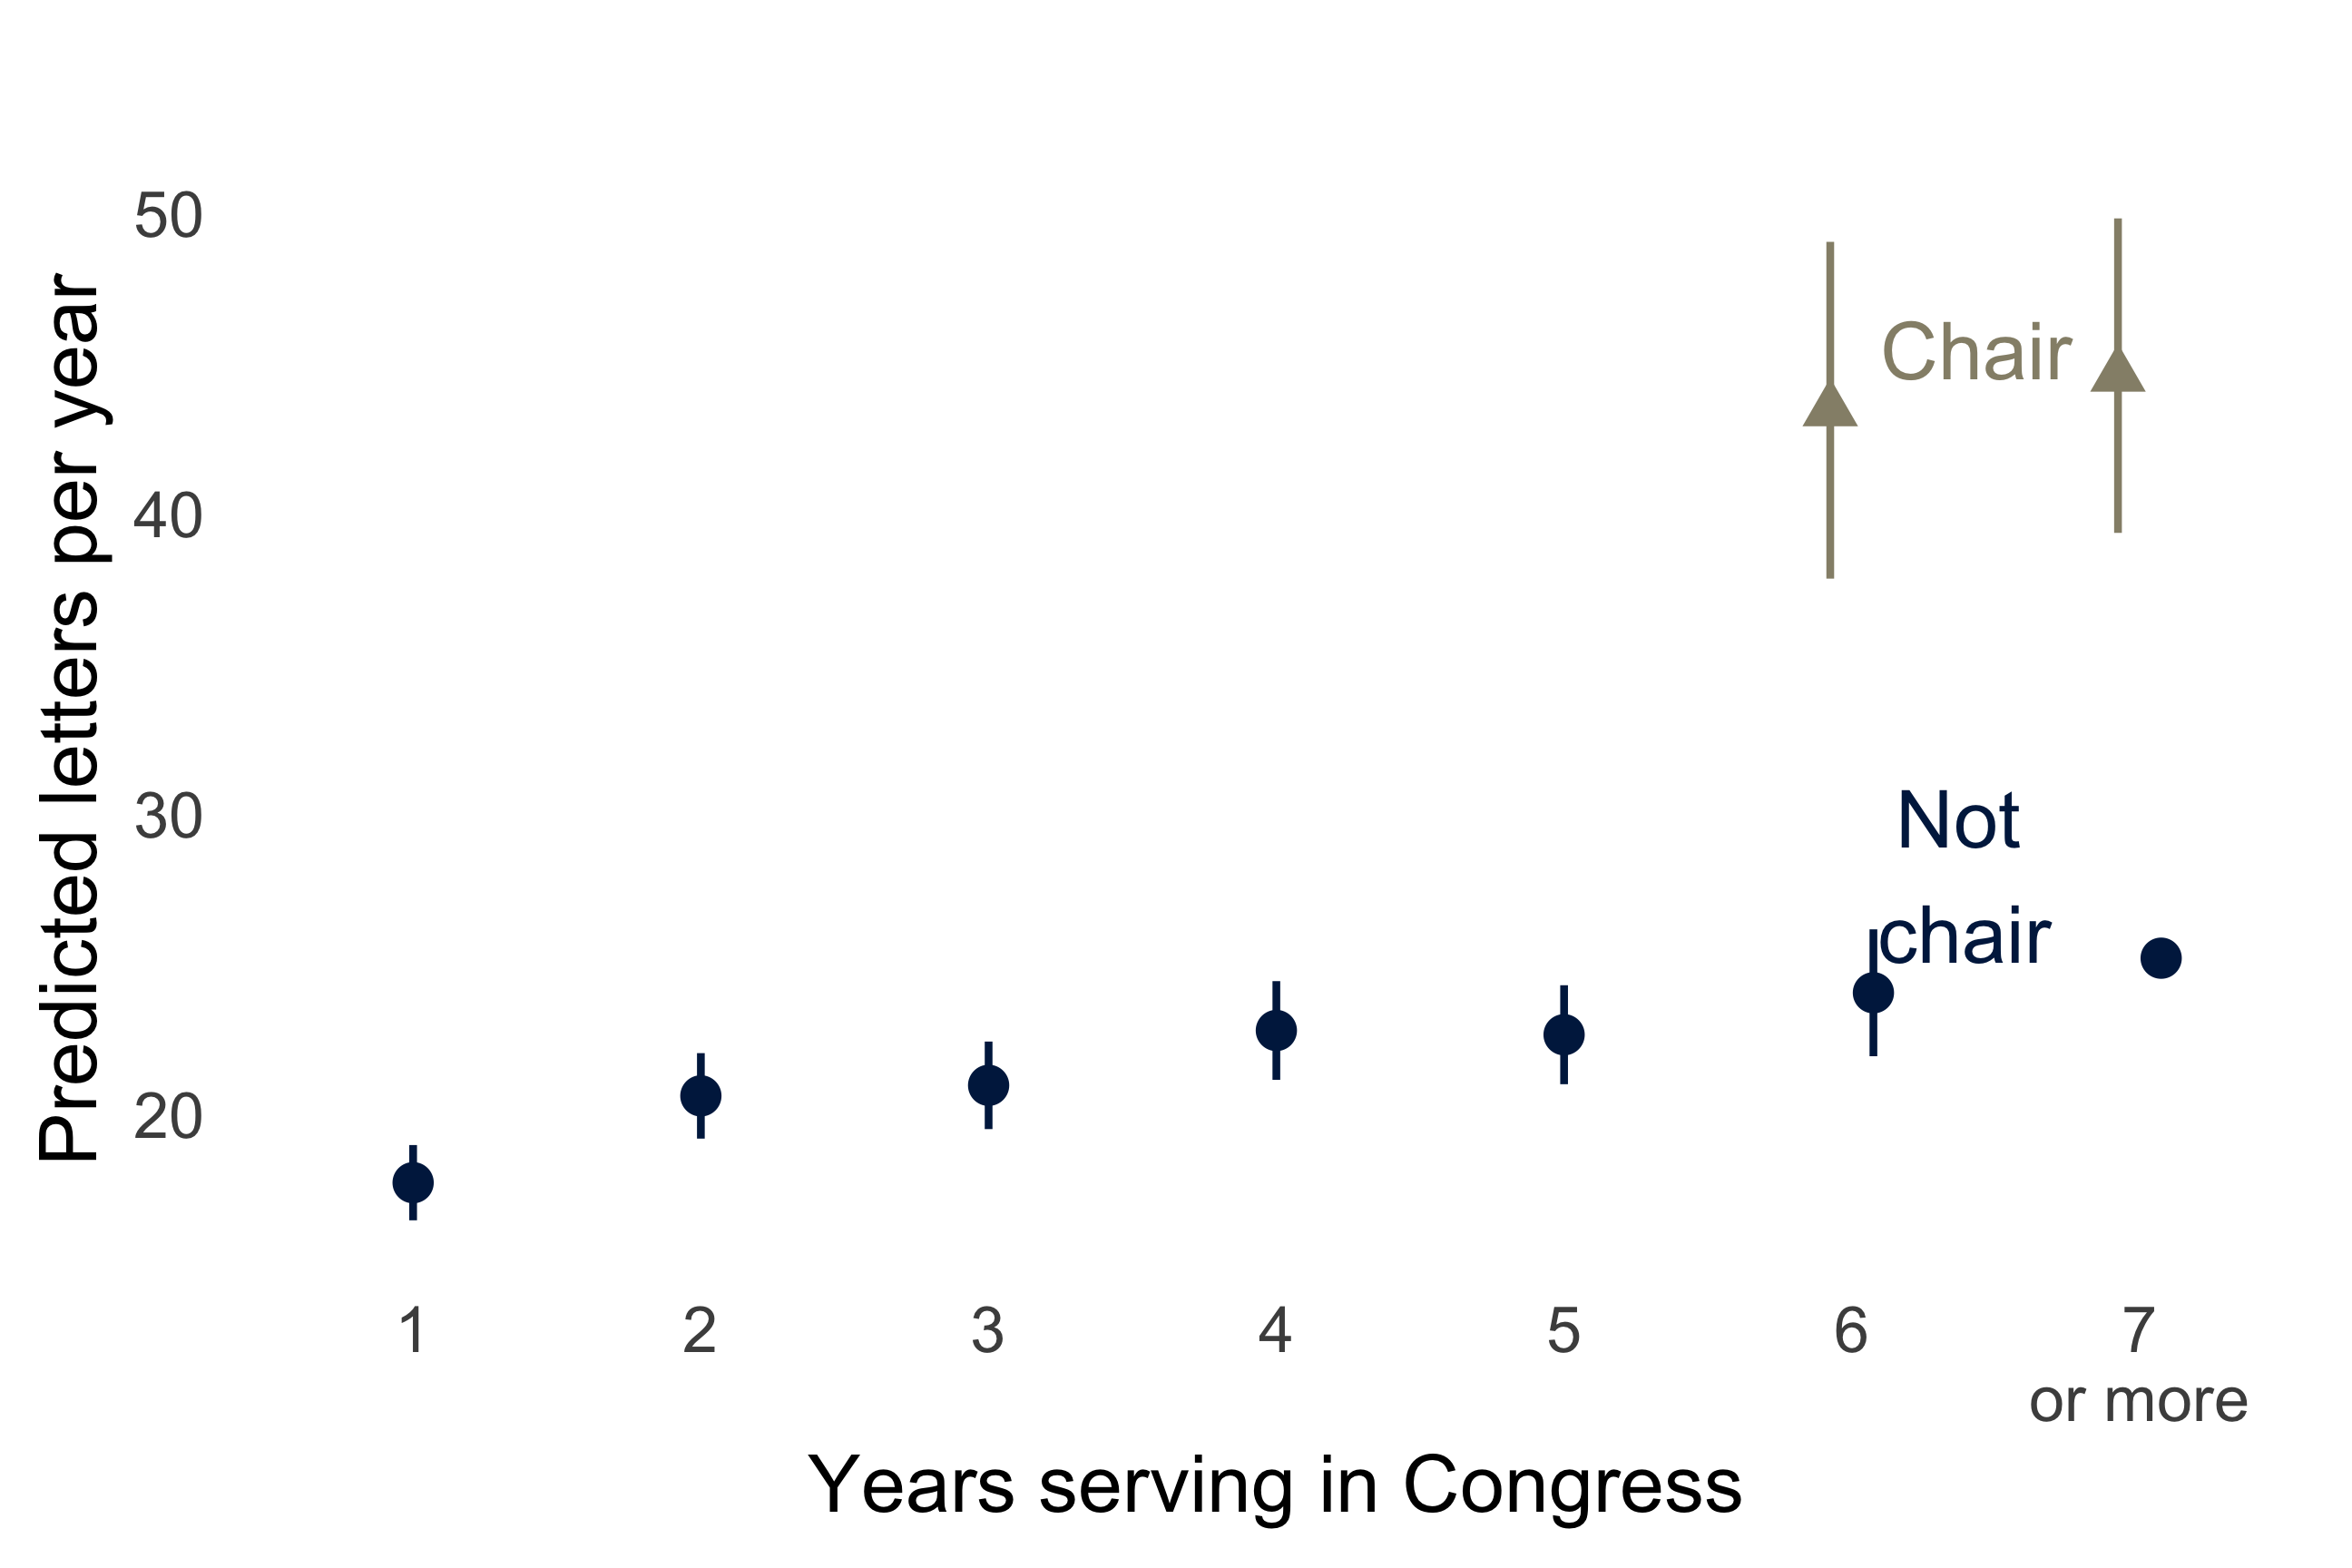
\includegraphics[width = .48\textwidth]{figs/m-policy-predicted-2} 
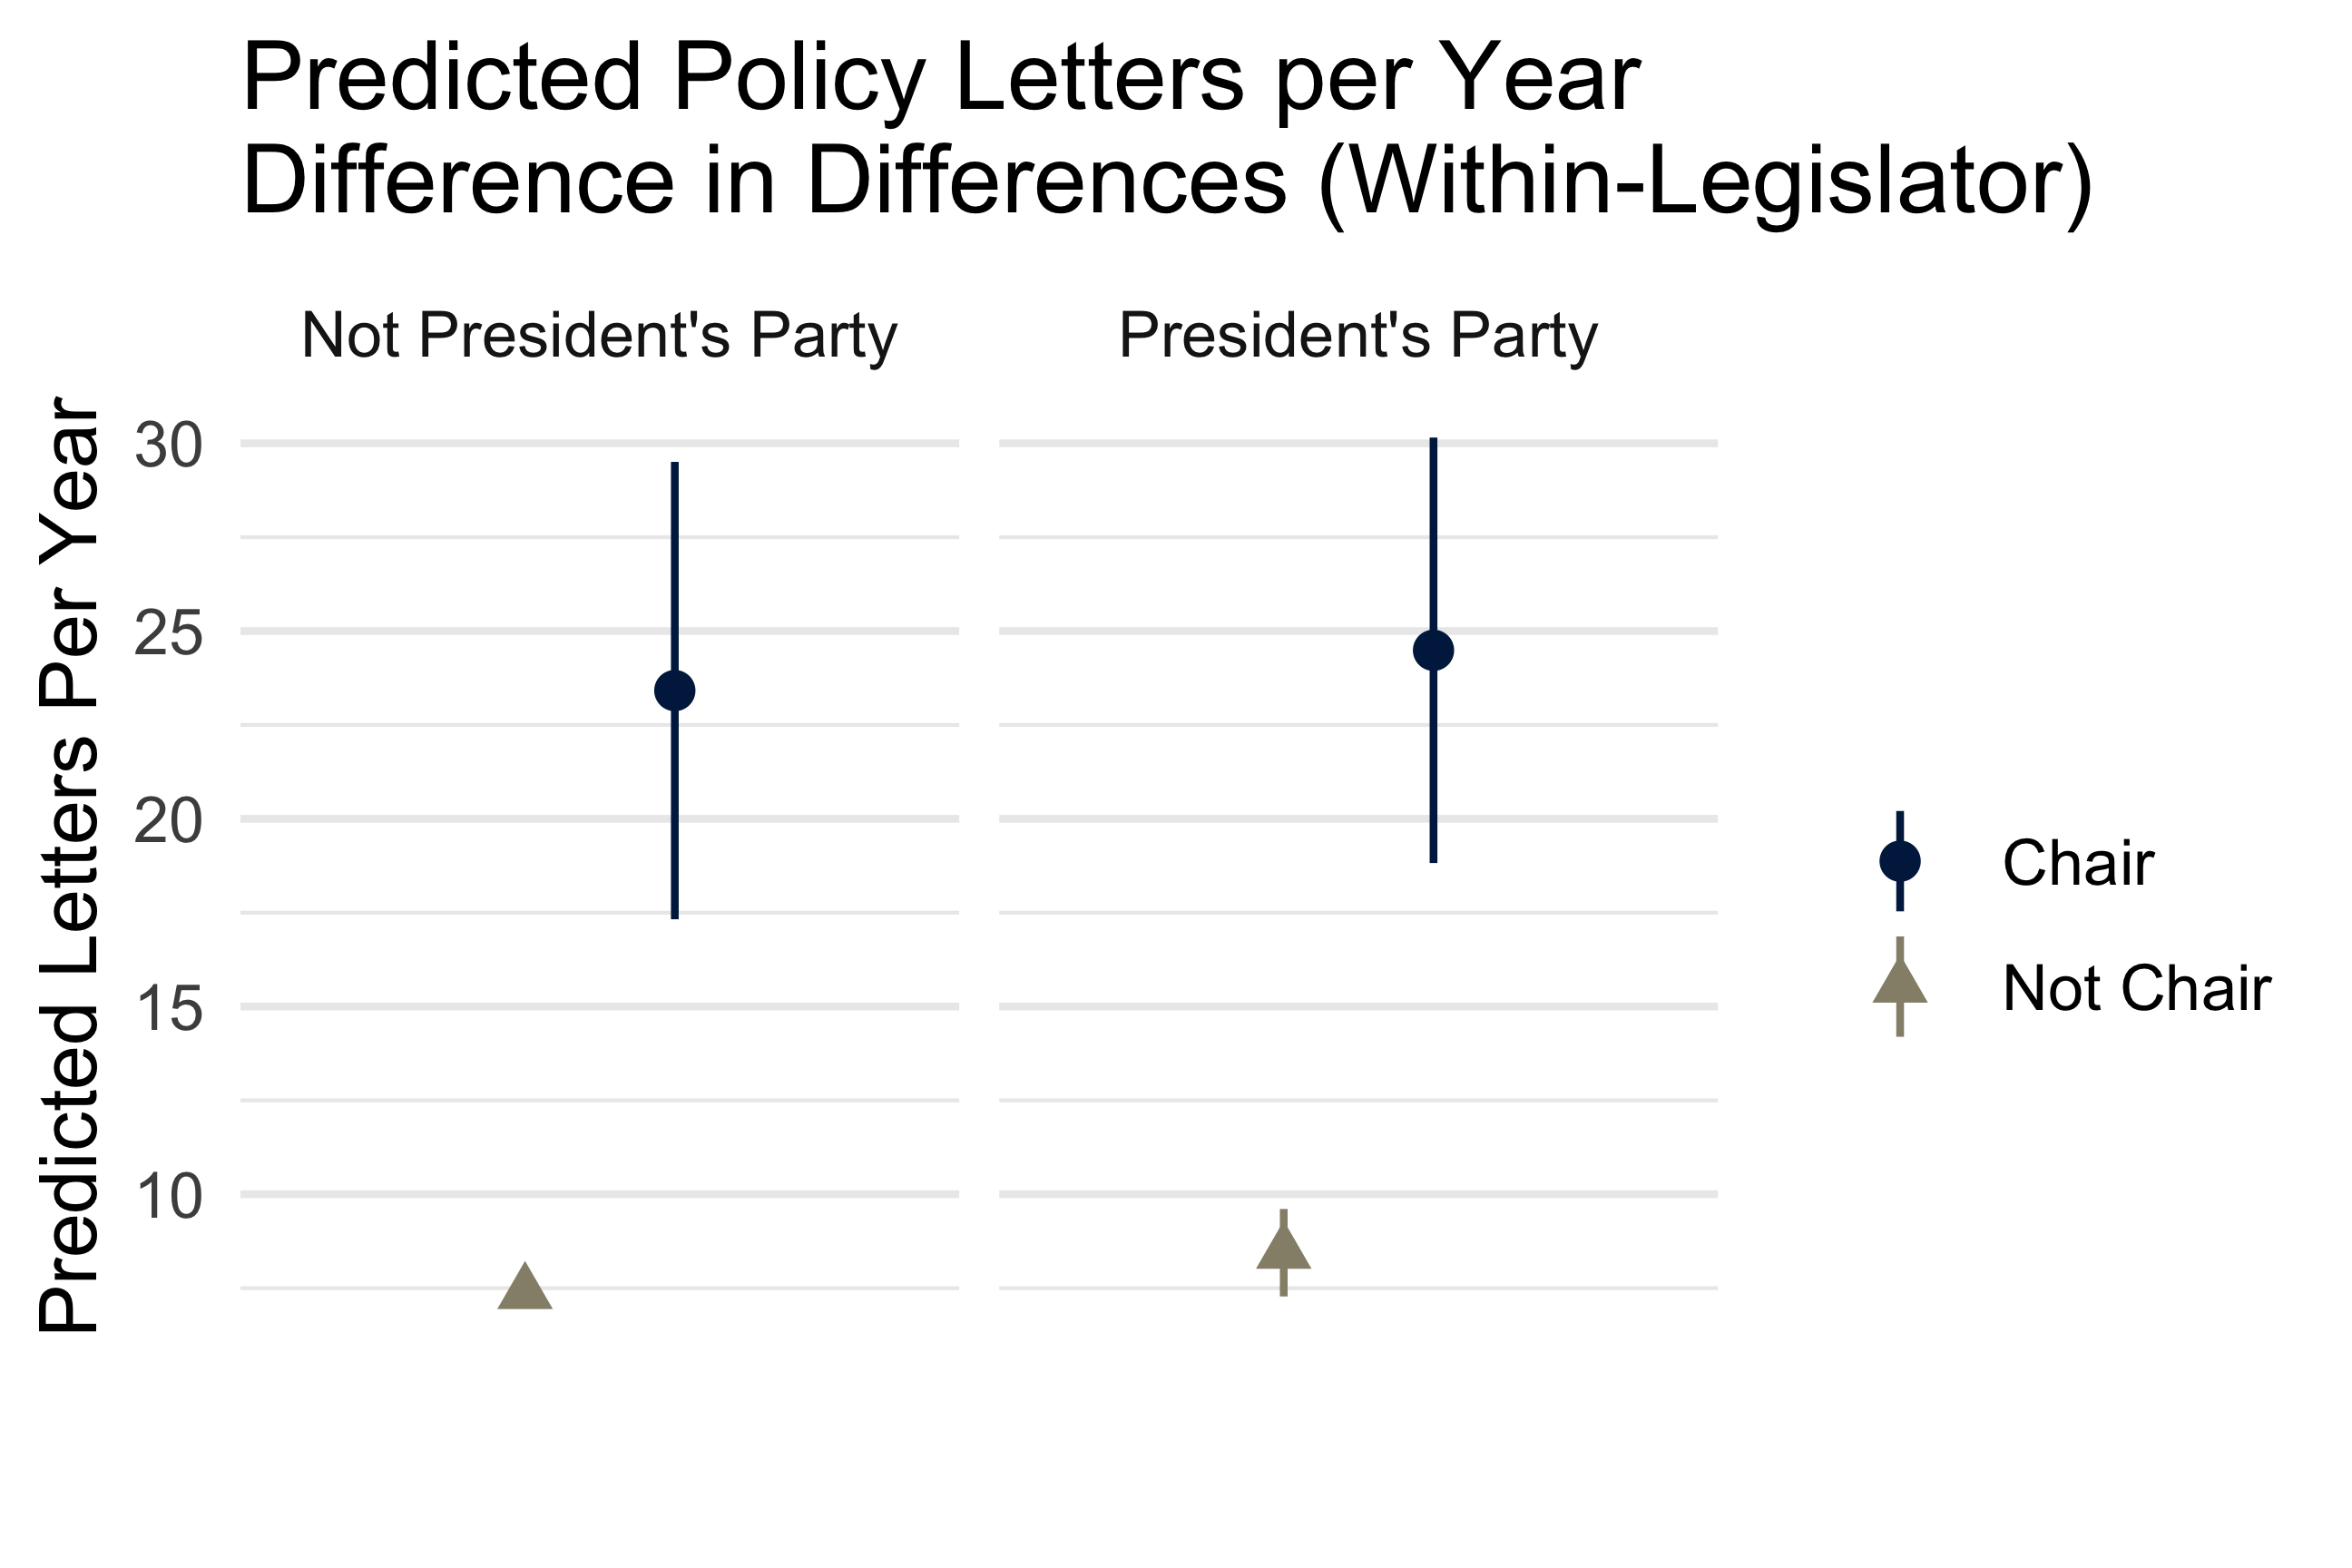
\includegraphics[width = .48\textwidth]{figs/m-policy-predicted-3} 
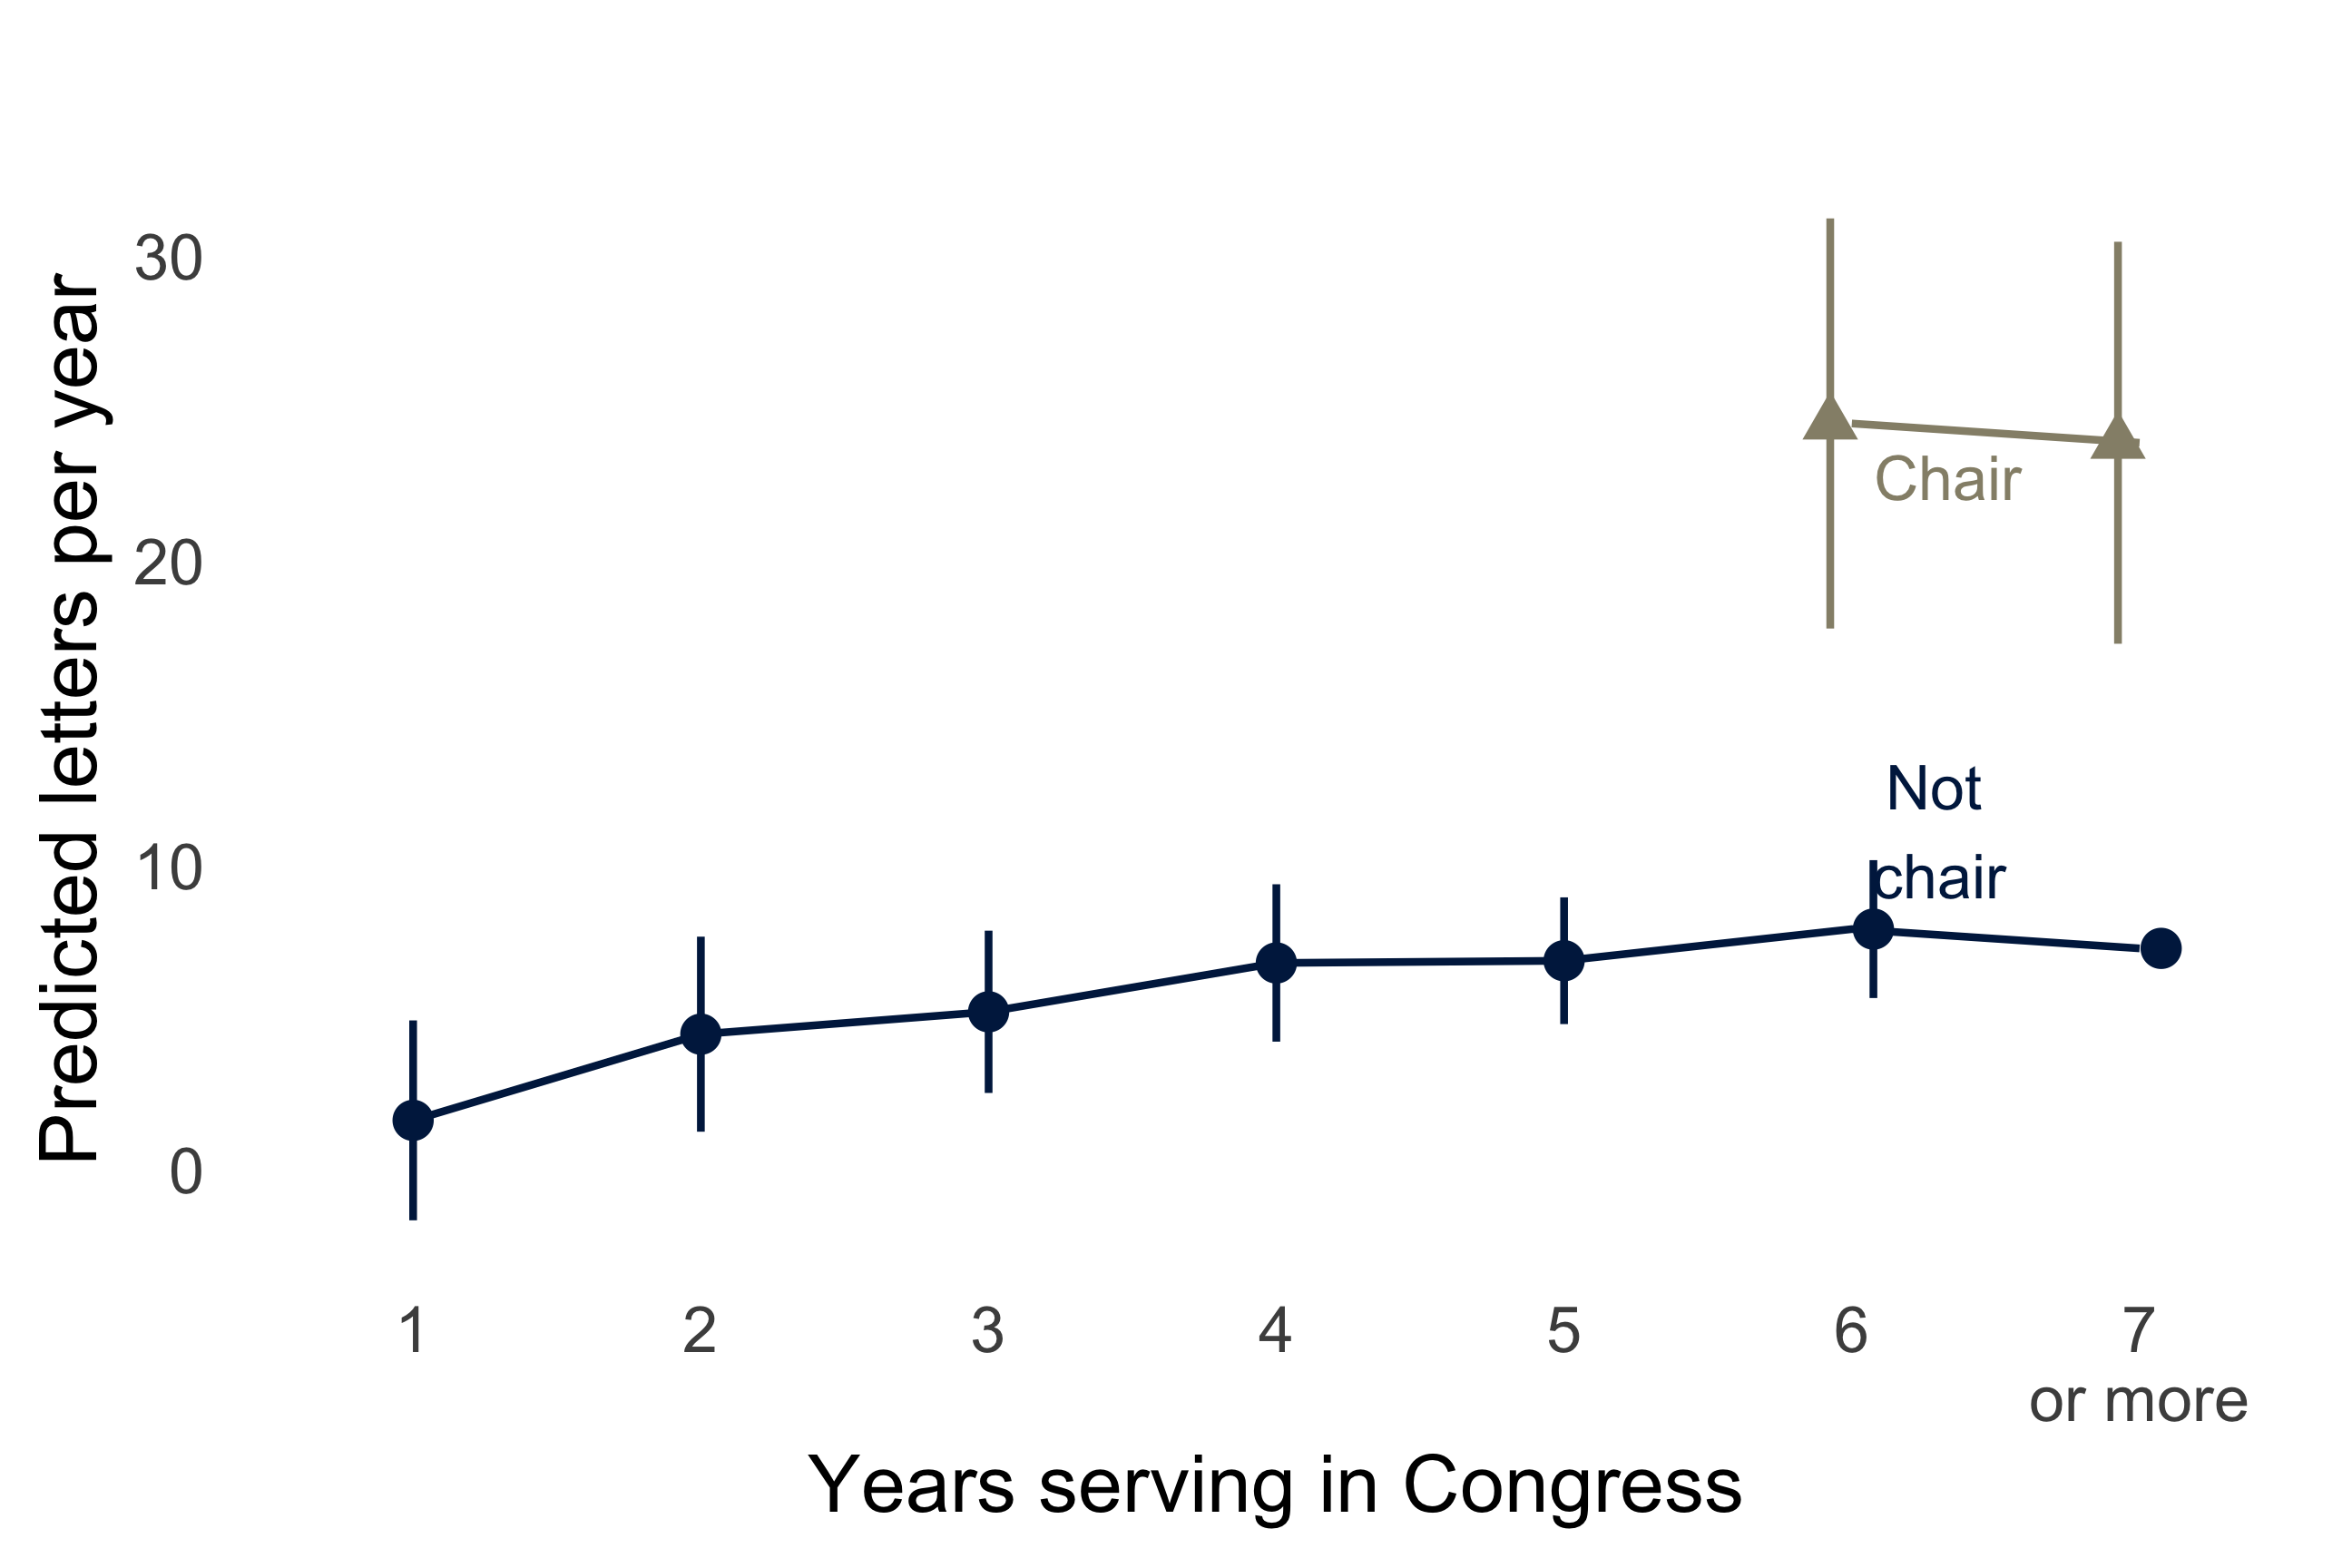
\includegraphics[width = .48\textwidth]{figs/m-policy-predicted-4} 

\end{figure}




\end{document}